\documentclass[11pt,a4paper,openany]{book}
\usepackage[normalem]{ulem}
\usepackage[T1]{fontenc}
\usepackage{iftex}
\ifPDFTeX
  \usepackage[utf8]{inputenc}
\fi
\usepackage[a4paper,margin=2.7cm]{geometry}
\usepackage{lmodern}
\usepackage{microtype}
\usepackage{xcolor}
\usepackage{amsmath,amssymb,amsthm}
\usepackage{mathtools}
\usepackage{array,booktabs,longtable,tabularx,multirow}
\newcommand{\proj}{\mathrm{proj}}
\usepackage{enumitem}
\usepackage{hyperref}
\usepackage[nameinlink,noabbrev]{cleveref}
\usepackage{listings}
\usepackage{tcolorbox}
\tcbuselibrary{breakable,skins,theorems}
\usepackage{makeidx}
\usepackage{titlesec}
\usepackage{fancyhdr}
\usepackage{graphicx}
\usepackage{adjustbox}
\usepackage{xurl}
\usepackage{float}
\usepackage{caption}
\usepackage{tikz}
\usetikzlibrary{arrows.meta,positioning,shapes.geometric,shapes.misc,fit,calc,backgrounds,decorations.markings,matrix,trees}

\makeindex

\definecolor{JYUblue}{HTML}{003A70}
\definecolor{JYUorange}{HTML}{FF6A00}
\definecolor{softblue}{HTML}{EEF4FB}
\definecolor{softorange}{HTML}{FFF4EC}
\definecolor{softgray}{HTML}{F6F6F6}
\definecolor{dkgreen}{rgb}{0,0.45,0}
\definecolor{mauve}{rgb}{0.58,0,0.82}

\hypersetup{
  colorlinks=true,
  linkcolor=JYUblue,
  citecolor=JYUblue,
  urlcolor=JYUblue,
  pdftitle={Introduction to Databases and Data Management},
  pdfauthor={Michael T. M. Emmerich}
}

\pagestyle{fancy}
\fancyhf{}
\fancyhead[LE,RO]{\thepage}
\fancyhead[LO]{\nouppercase{\rightmark}}
\fancyhead[RE]{\nouppercase{\leftmark}}
\setlength{\headheight}{28pt}
\fancyhead[LO]{\small\nouppercase{\rightmark}}
\fancyhead[RE]{\small\nouppercase{\leftmark}}
\emergencystretch=1.5em
\raggedbottom
% Keep chapter reading lists within their chapter, with unique link labels.
\makeatletter
\renewenvironment{thebibliography}[1]
 {\subsection*{References}%
  \list{\@biblabel{\@arabic\c@enumiv}}%
   {\settowidth\labelwidth{\@biblabel{#1}}%
    \leftmargin\labelwidth\advance\leftmargin\labelsep
    \usecounter{enumiv}\let\p@enumiv\@empty
    \renewcommand\theenumiv{\@arabic\c@enumiv}}%
  \sloppy\clubpenalty4000\widowpenalty4000}
 {\endlist}
\makeatother
\widowpenalty=10000
\clubpenalty=10000
\displaywidowpenalty=10000

\titleformat{\chapter}[display]
  {\normalfont\bfseries\color{JYUblue}}
  {\filleft\Huge\chaptername\ \thechapter}
  {1ex}
  {\titlerule[1pt]\vspace{1ex}\filright\Huge}
  [\vspace{1ex}\titlerule]

\setlist[itemize]{itemsep=0.3em,topsep=0.4em}
\setlist[enumerate]{itemsep=0.3em,topsep=0.4em}

\lstdefinestyle{sqlstyle}{
  language=SQL,
  basicstyle=\ttfamily\small,
  keywordstyle=\color{JYUblue}\bfseries,
  commentstyle=\color{dkgreen},
  stringstyle=\color{mauve},
  showstringspaces=false,
  breaklines=true,
  frame=single,
  rulecolor=\color{black!30},
  inputencoding=utf8,
  extendedchars=true,
  literate={ä}{{\"a}}1 {ö}{{\"o}}1 {å}{{\aa}}1 {Ä}{{\"A}}1 {Ö}{{\"O}}1 {Å}{{\AA}}1
}
\lstnewenvironment{codesql}{\endgraf\addvspace{0.5\baselineskip}\noindent\minipage{\linewidth}\lstset{style=sqlstyle}}{\endminipage\endgraf\addvspace{0.3\baselineskip}}

\newtcolorbox{guidancebox}{
  breakable,
  colback=softgray,
  colframe=JYUblue,
  title=Chapter guidance,
  fonttitle=\bfseries,
  boxrule=0.8pt,
  arc=2mm
}

\newtcolorbox{jokebox}{
  breakable,
  colback=softorange,
  colframe=JYUorange,
  title=Joke box,
  fonttitle=\bfseries,
  boxrule=0.8pt,
  arc=2mm
}

\newtcbtheorem[number within=chapter]{definition}{Definition}{
  enhanced,
  breakable,
  colback=softblue,
  colframe=JYUblue,
  fonttitle=\bfseries,
  coltitle=white,
  colbacktitle=JYUblue,
  arc=2mm,
  boxrule=0.8pt}{def}

\newtcbtheorem[number within=chapter]{theorem}{Theorem}{
  enhanced,
  breakable,
  colback=softblue,
  colframe=JYUblue,
  fonttitle=\bfseries,
  coltitle=white,
  colbacktitle=JYUblue,
  arc=2mm,
  boxrule=0.8pt}{thm}

\newtcbtheorem[number within=chapter]{remark}{Remark}{
  enhanced,
  breakable,
  colback=softgray,
  colframe=black!55,
  fonttitle=\bfseries,
  coltitle=white,
  colbacktitle=black!70,
  arc=2mm,
  boxrule=0.8pt}{rem}

\newtcbtheorem[number within=chapter]{example}{Example}{
  enhanced,
  breakable,
  colback=softorange,
  colframe=JYUorange,
  fonttitle=\bfseries,
  coltitle=white,
  colbacktitle=JYUorange,
  arc=2mm,
  boxrule=0.8pt}{ex}

\newcommand{\RAselect}{\sigma}
\newcommand{\RAproject}{\pi}
\newcommand{\RArename}{\rho}
\newcommand{\join}{\bowtie}
\newcommand{\natjoin}{\bowtie}


% TikZ styles and helpers imported from the lecture slides
\tikzset{
  er/entity/.style={draw, rounded corners=2pt, thick, minimum width=28mm, minimum height=9mm, align=center},
  er/weakentity/.style={er/entity, double, double distance=1.2pt},
  er/relationship/.style={draw, diamond, thick, aspect=1.8, inner sep=1.2pt, align=center, minimum width=18mm, minimum height=8mm},
  er/identrel/.style={er/relationship, double, double distance=1.2pt},
  er/attribute/.style={draw, ellipse, thick, inner sep=1.2pt, align=center, minimum width=18mm, minimum height=7mm},
  er/multival/.style={er/attribute, double, double distance=1.2pt},
  er/derived/.style={er/attribute, dashed},
  er/isa/.style={draw, circle, thick, inner sep=0pt, minimum size=6mm, align=center},
  er/line/.style={thick},
  er/card/.style={font=\footnotesize, inner sep=1pt, fill=white},
  er/note/.style={draw, rounded corners=2pt, thick, fill=black!2, inner sep=4pt, align=left},
  box/.style={draw,rounded corners,align=center,inner sep=4pt},
  soft/.style={draw,rounded corners,fill=black!3,align=center,inner sep=4pt},
  big/.style={draw,rounded corners,fill=JYUblue!6,align=center,inner sep=6pt},
  nodebig/.style={draw,rounded corners,fill=JYUblue!6,align=center,inner sep=6pt},
  arr/.style={-{Latex},thick},
  rel/table/.style={matrix of nodes,
    nodes={draw,text width=43mm,minimum height=5.4mm,align=left,font=\scriptsize,inner xsep=2pt,inner ysep=1.2pt},
    row 1/.style={nodes={fill=black, text=white, font=\bfseries\small, align=center}},
    row 2/.style={nodes={fill=black!10}}, row 3/.style={nodes={fill=black!2}},
    row 4/.style={nodes={fill=black!10}}, row 5/.style={nodes={fill=black!2}},
    row 6/.style={nodes={fill=black!10}}},
  rel/fk/.style={thick, -{Latex[length=2.2mm]}}
}
\newcommand{\keyattr}[1]{\underline{#1}}
\newcommand{\trow}[2]{\texttt{#1}\hfill\texttt{\textbf{#2}}}
\newcommand{\trowpk}[2]{\underline{\texttt{#1}}\hfill\texttt{\textbf{#2}}}
\newcommand{\stick}[3]{\begin{scope}[shift={(#1,#2)}]\draw[line width=0.9pt] (0,0.25) circle (0.18);\node[font=\scriptsize] at (0,0.25) {#3};\draw[line width=0.9pt] (0,0.07) -- (0,-0.55);\draw[line width=0.9pt] (-0.32,-0.15) -- (0.32,-0.15);\draw[line width=0.9pt] (0,-0.55) -- (-0.28,-0.95);\draw[line width=0.9pt] (0,-0.55) -- (0.28,-0.95);\end{scope}}
\newcommand{\stickman}[4]{\begin{scope}[shift={(#1,#2)}, scale=#3]\draw[line width=0.9pt] (0,0.25) circle (0.18);\node[font=\scriptsize] at (0,0.25) {#4};\draw[line width=0.9pt] (0,0.07) -- (0,-0.55);\draw[line width=0.9pt] (-0.32,-0.15) -- (0.32,-0.15);\draw[line width=0.9pt] (0,-0.55) -- (-0.28,-0.95);\draw[line width=0.9pt] (0,-0.55) -- (0.28,-0.95);\end{scope}}

\let\cleardoublepage\clearpage
\begin{document}

\frontmatter
\begin{titlepage}
\centering
{\Huge\bfseries Introduction to Databases and Data Management\par}
\vspace{1.5cm}
{\Large Companion reader for ISE-AI\par}
\vspace{2cm}
{\Large Michael T. M. Emmerich\par}
\vspace{0.5cm}
{\large Faculty of Information Technology\par}
{\large University of Jyväskylä\par}
\vfill
{\large Living book -- working edition\par}
\vspace{0.3cm}
{\large 7 October 2026\par}
\end{titlepage}

\chapter*{Preface}
This living book introduces databases and data management, from conceptual modeling and practical SQL to relational theory and distributed data systems. It accompanies the ISE-AI bachelor programme in Software Engineering and AI at the University of Jyväskylä, Faculty of Information Technology. It is intended for students new to databases and as a reference during software projects.

The book is supporting reading, with a broader scope and its own chapter order. The \href{https://tim.jyu.fi/view/kurssit/it/iseai/26-27/databases/home}{ISE-AI course home in TIM} defines the teaching sequence, assigned reading, exercises, assessment, and practical arrangements. A chapter's presence here does not make it required course content. In particular, the final chapter provides additional reading on Hadoop and MapReduce.

PostgreSQL is the database system used for SQL examples and practical work. Examples use ordinary PostgreSQL features; the implementation notes refer to the PostgreSQL 18 documentation. Relational algebra uses mathematical set semantics, while SQL normally retains duplicate rows. This distinction will matter throughout the book.

The nine chapters grew from the lecture slide sources maintained in the same repository. The reader now develops independently as a continuous text. The style uses explanations, worked examples, diagrams, review questions, and occasional jokes to connect database theory with practice.

\section*{How to use this edition}
Read actively: sketch the models, predict query results, and run the SQL in a practice database. Chapters 4 and 5 share a customer--invoice example. The repository includes a runnable setup and checks in \texttt{examples/}; illustrative alternatives and syntax templates are identified in the text. Examples that change data should be run in that practice environment.

The authoritative editable source is maintained on \href{https://github.com/emmerichmtm/DatabasesAndDataManagement}{GitHub}. This PDF is a dated snapshot, not a frozen textbook. Corrections and suggestions can be submitted as issues or pull requests. Cite the edition date and, when available, the Git commit or release tag so that others can locate the version you used.

\section*{Publication information}
Author: Michael T. M. Emmerich. Faculty of Information Technology, University of Jyväskylä. Working edition: 7 October 2026. This revision builds on repository commit \texttt{dab7a0d}.

Copyright \textcopyright\ Michael Emmerich. Shared under the \href{https://creativecommons.org/licenses/by/4.0/}{Creative Commons Attribution 4.0 International license (CC BY 4.0)}. Credit the author and identify changes when adapting the material.

\tableofcontents

\mainmatter

\chapter[Introduction]{Introduction: Databases and Data Management}
\begin{guidancebox}
This chapter introduces the course, the core vocabulary, and the reason databases matter. We begin with the big picture before moving to precise definitions. Read this chapter first if you want to understand what a database is, what a DBMS does, and why data management is much more than storing rows in a table.
\end{guidancebox}

\section{Why this course matters}
Almost every information system depends on stored data. A webshop stores customers and orders. A university system stores students, courses, and grades. A hospital stores patients, appointments, and treatments. A streaming service stores media, users, and recommendations. The data is often more valuable than the application code because the data captures the state of the organization and its activities.

A database  matters because data has to remain useful under pressure. The system must answer queries quickly, support many users at the same time, protect confidentiality, and avoid corruption. A good database design makes future work easier. A poor design makes every feature harder.

\section{Two systems with different requirements}
It is tempting to think that all data systems look alike. They do not. A small personal note app and a national tax system both store data, but their requirements are very different. One may care mainly about convenience. The other must care deeply about reliability, security, auditability, and legal correctness.

This contrast already teaches an important lesson: database design depends on context. There is no single perfect design for all settings. Instead, we choose structures and technologies that fit the workload and the risks.

\section{Course structure and study strategy}
A database course usually combines theory and practice. The theory explains what correct structure means. The practical side shows how to build and query database systems. In this manuscript, the flow is as follows:

\begin{enumerate}
\item We start with the basic idea of databases and data management.
\item We learn conceptual modeling with ER diagrams.
\item We move to the relational model.
\item We learn SQL for querying and database programming.
\item We study relational algebra as a formal query language.
\item We refine schemas with normal forms.
\item We broaden the view toward warehousing, distributed data, and big data systems.
\end{enumerate}

A useful way to study is to move repeatedly between concrete examples and general principles. When you meet a new term, ask both, ``What does it mean?'' and ``Where would I use it?''

Another good habit is to keep the three levels of modeling in mind while reading the book. In \cref{ch:er} we speak about the world in domain terms such as student, course, and invoice. In \cref{ch:relmodel} these ideas become relations, keys, and constraints. In \cref{ch:sqlbasic} and \cref{ch:sqlprog} we finally ask and update real data with SQL. Many confusions disappear once you ask yourself which level you are currently working on.

The field also has a human story. File systems and ad hoc programs did useful work, but they made data sharing painful. The early database pioneers wanted something more disciplined: a way to store data once, define meaning clearly, and let many applications use the same trusted source. That motivation still explains much of modern data management.

\section{A short history of information management}
Before database systems became dominant, many organizations used file based systems. Each application kept its own files in its own format. This often led to duplication, inconsistency, and hard to maintain software. The relational model changed this landscape by offering a clean logical structure, a strong theory, and a flexible query language.

Later, new needs appeared. Web scale systems, analytics, semi structured data, graph data, and streaming data pushed beyond the classic setting. Still, the relational model remains central because it offers clarity, discipline, and mature tooling. Even when organizations adopt non relational systems, they continue to rely on ideas developed in database theory.

\section{Key vocabulary}
\begin{definition}{Database}{database}
A \emph{database} is an organized collection of related data together with its intended meaning and structure.\index{database}
\end{definition}

\begin{definition}{DBMS}{dbms}
A \emph{database management system} or \emph{DBMS} is software that defines, stores, queries, updates, protects, and administers databases.\index{DBMS}
\end{definition}

\begin{definition}{Database system}{database-system}
A \emph{database system} consists of the database, the DBMS, the application programs, and the users or administrators who interact with them.\index{database system}
\end{definition}

A useful distinction is between \emph{data}, \emph{information}, and \emph{knowledge}. Data is raw recorded content. Information is data placed in context. Knowledge is understanding that supports action. Database systems mainly manage data, but they do so in ways that make information retrieval possible.

\section{Database versus random data}
Not every pile of files counts as a well managed database. A true database has structure, rules, and deliberate organization. Data is related. Meanings are known. Constraints define what is allowed. Queries return answers in a controlled way. Recovery mechanisms help after failures. Access rights restrict who may see or change what.

A spreadsheet can be useful, but it is usually not a DBMS. It lacks many of the mechanisms that serious multi user data management needs, such as concurrency control, transaction support, and schema based integrity enforcement.

\section{The tasks of a DBMS}
A DBMS performs many tasks at once:

\begin{itemize}
\item It stores data efficiently on persistent media.
\item It offers data definition tools for schemas and constraints.
\item It supports queries and updates.
\item It manages concurrent access by many users.
\item It recovers from crashes.
\item It enforces security and access control.
\item It provides administration tools, such as backup and performance tuning.
\end{itemize}

\section{Levels of data models}
Database thinking often distinguishes three levels. The \emph{conceptual level} describes the domain in human terms. The \emph{logical level} describes the formal database structure, for example with relations and keys. The \emph{physical level} describes how data is actually stored and accessed on hardware.

\begin{definition}{Data model}{data-model}
A \emph{data model} is a collection of concepts used to describe the structure of data, relationships between data items, allowed constraints, and often supported operations.\index{data model}
\end{definition}

The same application may have all three levels. A university domain may be modeled conceptually with students and courses, logically with tables and foreign keys, and physically with files, pages, and indexes.



\begin{center}
\begin{tikzpicture}[
    box/.style={draw,rounded corners,minimum width=3.1cm,minimum height=0.9cm,align=center},
    arr/.style={-{Latex},thick}
  ]
    \node[box] (users) {Users};
    \node[box,below=0.55cm of users] (app) {Application\\(logic + UI)};
    \node[box,below=0.55cm of app] (dbms) {DBMS};
    \node[box,below=0.55cm of dbms] (db) {Database\\(schema + data)};
    \draw[arr] (users) -- (app);
    \draw[arr] (app) -- (dbms);
    \draw[arr] (dbms) -- (db);
\end{tikzpicture}

\small A lecture figure showing the system stack that turns user requests into persistent storage operations.
\end{center}

\begin{center}
\resizebox{0.9\textwidth}{!}{\begin{tikzpicture}[
  box/.style={draw,rounded corners,minimum width=3.0cm,minimum height=1.0cm,align=center},
  arr/.style={-{Latex},thick}]
\node[box] (domain) {Domain\\(requirements)};
\node[box,right=0.7cm of domain] (concept) {Conceptual\\(ER)};
\node[box,right=0.3cm of concept] (logical) {Logical\\(relational)};
\node[box,right=0.7cm of logical] (physical) {Physical\\(indexes, storage)};
\draw[arr] (domain) -- (concept);
\draw[arr] (concept) -- (logical);
\draw[arr] (logical) -- (physical);
\end{tikzpicture}}

\small This is the path followed by the course: from requirements to conceptual modeling, then to the relational schema and finally to implementation details.
\end{center}

\section{PostgreSQL as the learning environment}
PostgreSQL gives us one consistent environment for table definitions, queries, constraints, views, indexes, roles, and transactions. It runs as a database server; tools such as \texttt{psql} or pgAdmin connect to that server. A client application is therefore distinct from the DBMS itself.

Use the connection and installation instructions supplied in TIM. Create a practice database and run the repository's example setup there. Other SQL systems use many of the same ideas, but syntax, types, and transaction behavior can differ. When a result is surprising, consult the PostgreSQL documentation for the feature and version in use.

\section{Records, metadata, and data management}
A \emph{record} is a structured unit of stored information. \emph{Metadata} is data about data, for example schema definitions, column types, or access permission information. \emph{Data management} is the broader discipline that includes modeling, storage, querying, quality control, governance, integration, and lifecycle issues.

Data management matters because data does not stay still. It is created, changed, copied, merged, audited, archived, and reused. Good data management therefore aims not only at storage, but also at long term trustworthiness.

\section{Review questions and small exercises}
\begin{enumerate}
\item Explain the difference between a database, a DBMS, and a database system.
\item Why is a spreadsheet usually not considered a full DBMS?
\item Give one example of a conceptual, logical, and physical description for the same application.
\item Why does database design depend on context? Illustrate with two different applications.
\item What role does metadata play in data management?
\item List four important tasks of a DBMS and explain why each matters.
\item What is the difference between the PostgreSQL server and a client such as \texttt{psql}?
\end{enumerate}

\section{Further reading}
This chapter gives the broad entry point to the subject. For a classical and very influential treatment of database concepts and architecture, the text by Elmasri and Navathe is a standard starting point. Silberschatz, Korth, and Sudarshan give a balanced introduction with both systems and theory. Ramakrishnan and Gehrke provide many practical examples and a clean explanation of why database design choices matter.

\begin{thebibliography}{9}
\bibitem{ch1-elmasri}
R. Elmasri and S. B. Navathe.
\textit{Fundamentals of Database Systems}. Pearson.
\bibitem{ch1-silberschatz}
A. Silberschatz, H. F. Korth, and S. Sudarshan.
\textit{Database System Concepts}. McGraw-Hill.
\bibitem{ch1-ramakrishnan}
R. Ramakrishnan and J. Gehrke.
\textit{Database Management Systems}. McGraw-Hill.
\end{thebibliography}

\section{Wrap-up}
This chapter introduced the purpose of database systems and the vocabulary used in the rest of the book. The next chapter moves one step earlier in the design process. Before we create tables, we first model the real world that the database should represent.

\chapter[Conceptual Modeling]{Conceptual Modeling with ER Diagrams}
\label{ch:er}
\begin{guidancebox}
This chapter is about modeling the world before we decide on tables. It explains entities, attributes, relationships, cardinality constraints, weak entities, and extended ER features such as specialization and aggregation. Read it as the bridge between informal requirements and formal design.
\end{guidancebox}

\section{Why conceptual modeling comes first}
A database should represent a domain, not just a software convenience. If we rush directly to tables, we may hard code accidental choices too early. Conceptual modeling gives a cleaner start. It asks what kinds of objects exist, what properties they have, and how they are related.

ER modeling is especially useful when talking to domain experts. The notation is more human friendly than SQL and more precise than a paragraph of prose.

This is one reason conceptual modeling usually comes before implementation. A hospital expert may be able to tell us that a patient can have many appointments, that an appointment belongs to exactly one patient, and that some appointments may later be cancelled. That person may not care yet whether the final system uses SQLite, PostgreSQL, or a cloud platform. ER modeling lets us talk about the meaning first.

Historically, this chapter is closely connected with the work of Peter Chen, who introduced the entity relationship model in the 1970s. The lasting success of the model comes from its balance: it is simple enough for discussion, yet structured enough to guide later formal design. The next chapter will show exactly how these modeling choices are turned into relations and keys.

\section{Structure of a database system}
Let us briefly look how this fits into the bigger picture of a database design.
At a high level, users or applications send commands to the DBMS. The DBMS interprets these commands, checks schemas and permissions, accesses stored data, and returns results. A conceptual model does not show all internal DBMS machinery, but it helps define what the data should mean before implementation details enter the picture.

A DBMS is expected to provide more than just storage. It should support create, read, update, and delete operations, concurrent use by many users, integrity, and a degree of physical and logical data independence. In other words, the designer should be able to improve storage structures or implementation details later without changing the meaning of the data model every time. This is one reason why conceptual design should be kept separate from low-level implementation choices.

\begin{figure}[tbp]
\centering
\begin{adjustbox}{max width=0.62\linewidth,max totalheight=0.42\textheight,center}
\begin{tikzpicture}[scale=0.9, transform shape,node distance=3mm and 9mm]
  \node[er/note, minimum width=35mm] (req) {Request /\\Query};
  \node[draw, thick, rounded corners=2pt, below=of req, minimum width=35mm, align=center] (conn) {Connection\\(accept/deny)};
  \node[draw, thick, rounded corners=2pt, below=of conn, minimum width=35mm, align=center] (parser) {Parser};
  \node[draw, thick, rounded corners=2pt, below=of parser, minimum width=35mm, align=center] (rew) {Rewriter};
  \node[draw, thick, rounded corners=2pt, below=of rew, minimum width=35mm, align=center] (opt) {Optimizer};
  \node[draw, thick, rounded corners=2pt, below=of opt, minimum width=35mm, align=center] (run) {Runner};

  \draw[-{Latex}, thick] (req) -- (conn);
  \draw[-{Latex}, thick] (conn) -- (parser);
  \draw[-{Latex}, thick] (parser) -- (rew);
  \draw[-{Latex}, thick] (rew) -- (opt);
  \draw[-{Latex}, thick] (opt) -- (run);
\end{tikzpicture}
\end{adjustbox}
\caption{A high-level flow of a database command inside a DBMS. A request is accepted or rejected, parsed, rewritten, optimized, and then executed.}
\label{fig:dbms-command-flow}
\end{figure}

Although \Cref{fig:dbms-command-flow} is simplified, it is pedagogically useful. It reminds us that the user sees queries and results, but inside the DBMS there are several layers. Conceptual modeling belongs before these inner stages. It clarifies what the data means so that later query processing, optimization, integrity checks, and storage decisions are built on a sound foundation.

\section{Conceptual modelling}
Conceptual modelling is an early stage of database design. At this stage we identify domain concepts, constraints, and assumptions, but we do not yet commit to one concrete implementation model. In that sense conceptual modeling is data-model independent. The goal is to distinguish essential data from non-essential detail and to make assumptions explicit.

The ER model is the classical tool for this stage. It gives a vocabulary for talking about the domain in terms of things, properties, and associations. Later, the relational model will translate these ideas into tables, keys, foreign keys, and constraints. For now, however, we focus on understanding the real world that the database should describe.

\section{Entity sets and attributes}

Roughly speaking, in the ER diagram, entities refer to objects of the real world. In an entity set they are of the same type and they share the same attributes, unless inheritance is considered. Relationship sets contain relationships between entities, and the relationships in one relationship set connect entities of the same participating types and roles. The actual entity instances may differ.

\begin{definition}{Entity and entity set}{entity-set}
An \emph{entity} is a distinguishable object in the domain of discourse. An \emph{entity set} is a collection of similar entities, such as all students or all courses. Entities of the same entity set have the same attributes (see next definition). \index{entity set}
\end{definition}

\begin{definition}{Attribute}{attribute}
An \emph{attribute} is a property used to describe an entity or relationship, such as a student's name or a course's credit count.\index{attribute}
\end{definition}

For example, in a student information system, \texttt{STUDENT} may be an entity set with attributes \texttt{StudentId}, \texttt{FirstName}, \texttt{LastName}, and \texttt{DateOfBirth}. \Cref{fig:er-student-basic} shows this classic Chen style pattern: a rectangle for the entity set, ovals for attributes, and an underlined key attribute.

\begin{figure}[tbp]
\centering
\begin{adjustbox}{max width=0.72\linewidth,max totalheight=0.28\textheight,center}
\begin{tikzpicture}[scale=0.9, transform shape,node distance=6mm and 8mm]
  \node[er/entity] (student) {STUDENT};
  \node[er/attribute, above left=of student] (fn) {FirstName};
  \node[er/attribute, left=of student] (ln) {LastName};
  \node[er/attribute, above=of student] (id) {\keyattr{StudentId}};
  \node[er/attribute, above right=of student] (dob) {DateOfBirth};
  \draw[er/line] (student) -- (fn);
  \draw[er/line] (student) -- (ln);
  \draw[er/line] (student) -- (id);
  \draw[er/line] (student) -- (dob);
\end{tikzpicture}
\end{adjustbox}
\caption{A basic ER fragment with one entity set, several attributes, and an underlined key attribute.}
\label{fig:er-student-basic}
\end{figure}

The figure also illustrates a practical point: an ER diagram should use names from the domain, not from accidental software choices. A domain expert naturally understands words such as \texttt{STUDENT}, \texttt{COURSE}, and \texttt{CompletionDate}. The later database implementation may rename, abbreviate, or encode things differently, but good conceptual models keep the meaning visible.

\section{Key attributes}
\begin{definition}{Key attribute}{key-attribute}
A \emph{key attribute} is an attribute whose values uniquely identify entities within an entity set.\index{key attribute} In the ER diagram it is underlined. Sometimes, multiple attributes in combination form a key. Then they are all underlined in the ER diagram. The combination is called a composite key.
\end{definition}

Names often do not work as keys because they are not guaranteed to be unique. A student number is usually a better choice. In ER diagrams, a key attribute is underlined. A strong entity type may have several candidate keys; the diagram underlines the chosen identifier. A weak entity instead needs its owner's key together with a partial key. Choose identifiers from explicit domain rules: even \texttt{Name} together with \texttt{BirthDate} is not guaranteed to distinguish every person.

A practical warning is that safe key management can become difficult in large-scale databases. A theoretically unique attribute is not always a practically good key. Good keys should be stable, easy to manage, and hard to confuse. This is why designers often prefer identifiers such as \texttt{StudentId} rather than names alone. The problem is not merely technical. A poor key choice creates errors in identity, merging, deduplication, and updates.

\section{Composite, derived, and multivalued attributes}
Some attributes have internal structure. An address can be split into street, postal code, and city. Such an attribute is called \emph{composite}. Some attributes can be derived from others. Age can be derived from date of birth. Such an attribute is \emph{derived}. Some attributes can have several values for one entity, such as multiple phone numbers. These are \emph{multivalued attributes}.\index{multivalued attribute}\index{derived attribute}\index{composite attribute}

These distinctions matter because not every concept should be stored in the same way. Derived values, for example, are often better computed than stored. Multivalued attributes are also a warning sign. They often indicate that the later relational design may need a separate relation instead of trying to pack several values into one field. \Cref{fig:er-attribute-types} links the three ideas directly to their ER notation.

\begin{figure}[tbp]
\centering
\begin{adjustbox}{max width=0.95\linewidth,max totalheight=0.28\textheight,center}
\begin{tikzpicture}[scale=0.82, transform shape]
  \node[er/entity] (person) at (0,0) {PERSON};
  \node[er/attribute] (addr) at (0,-1.6) {Address};
  \node[er/attribute] (street) at (-1.9,-3.0) {Street};
  \node[er/attribute] (city) at (0,-3.0) {City};
  \node[er/attribute] (zip) at (2.9,-3.0) {PostalCode};
  \draw[er/line] (person) -- (addr);
  \draw[er/line] (addr) -- (street);
  \draw[er/line] (addr) -- (city);
  \draw[er/line] (addr) -- (zip);

  \node[er/entity] (student) at (6.4,0) {STUDENT};
  \node[er/derived] (age) at (5.0,1.5) {Age};
  \node[er/multival] (phone) at (8.2,1.5) {Phone};
  \node[er/multival] (email) at (10.2,0.2) {Email};
  \node[er/attribute] (dbirth) at (5.0,-1.5) {DateOfBirth};
  \draw[er/line] (student) -- (age);
  \draw[er/line] (student) -- (phone);
  \draw[er/line] (student) -- (email);
  \draw[er/line] (student) -- (dbirth);
\end{tikzpicture}
\end{adjustbox}
\caption{Composite, derived, and multivalued attributes in ER notation. Address is composite, Age is derived, and Phone and Email are multivalued.}
\label{fig:er-attribute-types}
\end{figure}

A useful modeling habit is to ask what should really be stored and what can be computed when needed. Age changes over time, while date of birth does not. That makes \texttt{DateOfBirth} the more stable fact. Similarly, a multivalued attribute may be acceptable in a conceptual diagram, but it should make the designer alert. In later chapters we will see why repeating values fit badly into flat relations.

\section{Relationship sets}
\begin{definition}{Relationship set}{relationship-set}
A \emph{relationship set} describes associations among entities, such as a student enrolling in a course or an employee working in a department.\index{relationship set}
\end{definition}

A binary relationship connects two entity sets. A ternary relationship connects three. Ternary relationships should not be replaced casually by several binary ones, because meaning may be lost. For example, the fact that a teacher evaluates a student in a course is naturally ternary.

Two practical details are important here. First, relationship sets are often named by verb phrases, because they describe how entities are associated. Second, a relationship set may itself have attributes. For example, if a student completes a course, then \texttt{CompletionDate} belongs naturally to the relationship rather than to the student or the course alone. In this way a relationship set can be understood as a set of tuples such as \((s,c,d)\), where \(s \in \texttt{STUDENT}\), \(c \in \texttt{COURSE}\), and \(d\) belongs to a suitable date domain.

\begin{figure}[tbp]
\centering
\begin{adjustbox}{max width=0.70\linewidth,max totalheight=0.28\textheight,center}
\begin{tikzpicture}[scale=0.92, transform shape,node distance=8mm and 10mm]
  \node[er/entity] (stud) {STUDENT};
  \node[er/entity, right=18mm of stud] (course) {COURSE};
  \node[er/relationship, above=10mm of $(stud)!0.5!(course)$] (comp) {Completes};
  \node[er/attribute, above=of comp] (date) {CompletionDate};
  \draw[er/line] (stud) -- (comp);
  \draw[er/line] (course) -- (comp);
  \draw[er/line] (comp) -- (date);
\end{tikzpicture}
\end{adjustbox}
\caption{A relationship set may have attributes of its own. Here CompletionDate belongs to the relationship Completes rather than to STUDENT or COURSE alone.}
\label{fig:er-relationship-attribute}
\end{figure}

\Cref{fig:er-relationship-attribute} is important because it prevents a common modeling mistake. If \texttt{Completion\allowbreak Date} were attached to \texttt{STUDENT}, it would suggest one completion date per student. If it were attached to \texttt{COURSE}, it would suggest one completion date per course. Neither expresses the intended meaning. The attribute belongs to the relationship instance.

\section{Degree of a relationship}
The \emph{degree} (arity) of a relationship is the number of participating entity roles. A recursive binary relationship such as supervision has two roles from the same entity type. Such a relationship is also called unary in conventions that count distinct participating types. Binary and ternary relationships have two and three roles, respectively; state which convention is in use. The degree matters because it affects both meaning and later translation into relations.

\begin{figure}[tbp]
\centering
\begin{minipage}[t]{0.47\linewidth}
\centering
\begin{adjustbox}{max width=\linewidth,max totalheight=0.24\textheight,center}
\begin{tikzpicture}[scale=0.92, transform shape,node distance=8mm and 10mm]
  \node[er/entity] (emp) {EMPLOYEE};
  \node[er/relationship, below=18mm of emp] (sup) {Supervises};

  \draw[er/line] (emp) -- (sup)
    node[midway, left, er/card] {supervisor};

  \draw[er/line]
    (emp.east) .. controls +(8mm,-8mm) and +(8mm,8mm) .. (sup.east)
    node[midway, right, er/card] {subordinate};
\end{tikzpicture}
\end{adjustbox}
\caption{A unary relationship. EMPLOYEE participates twice in Supervises, once in the role supervisor and once in the role subordinate.}
\label{fig:er-unary-supervises}
\end{minipage}\hfill
\begin{minipage}[t]{0.47\linewidth}
\centering
\begin{adjustbox}{max width=\linewidth,max totalheight=0.24\textheight,center}
\begin{tikzpicture}[scale=0.88, transform shape,node distance=7mm and 12mm]
  \node[er/entity] (teacher) {PRODUCT};
  \node[er/entity, right=20mm of teacher] (student) {CLIENT};
  \node[er/entity, below=12mm of $(teacher)!0.5!(student)$] (course) {SHOP};
  \node[er/relationship, above=8mm of course] (grade) {Buys};

  \draw[er/line] (teacher) -- (grade);
  \draw[er/line] (student) -- (grade);
  \draw[er/line] (course) -- (grade);
\end{tikzpicture}
\end{adjustbox}
\caption{A ternary relationship. The fact that a client buys a product in a particular shop is not captured by separate binary relationships alone.}
\label{fig:er-ternary-buys}
\end{minipage}
\end{figure}

\Cref{fig:er-unary-supervises} shows a unary relationship with role names. Such labels are helpful because one entity set can participate in more than one role. \Cref{fig:er-ternary-buys} shows a ternary relationship. A ternary relationship is not, in general, equivalent to three binary ones. If we split the ternary fact into separate binary associations, we may lose which product was bought by which client in which shop. If the domain really requires the joint fact, the ternary relationship is the honest model.

\section{Degree and participation}
Participation constraints describe whether participation is optional or mandatory, while cardinality constraints specify how often an entity may take part in a relationship. For example, if the participation of entity set \(A\) in a relationship set \(R\) has cardinality \((N,M)\), then each entity in \(A\) must participate in at least \(N\) and at most \(M\) relationship instances of \(R\). Together, these constraints capture patterns such as one-to-one, one-to-many, and many-to-many.\index{cardinality}

These constraints are important because they later influence the relational design. A one-to-many relationship is translated differently from a many-to-many relationship. The worked example in \cref{fig:er-worked-mini-example} makes these cardinalities visible instead of leaving them as prose alone.

A helpful practical formulation is this: ask how many times an entity from a given entity set must participate, and how many times it may participate, in the relationship set. This simple question often resolves modeling uncertainty. The minimum is often \(0\) or \(1\), and the maximum is often \(1\) or \(N\), but more specific ranges are also possible.

\section{Cardinality: min and max participation}
Cardinality expresses \emph{how many} entities can or must participate in a relationship. We usually place a minimum and maximum near each participating entity set. The minimum tells us whether participation is optional or mandatory. The maximum tells us whether one or many relationship instances are possible.

\begin{figure}[tbp]
\centering
\begin{minipage}[t]{0.47\linewidth}
\centering
\begin{adjustbox}{max width=\linewidth,max totalheight=0.22\textheight,center}
\begin{tikzpicture}[scale=0.92, transform shape,node distance=8mm and 18mm]
  \node[er/entity] (person) {PERSON};
  \node[er/entity, right=42mm of person] (car) {CAR};
  \node[er/relationship] (owns) at ($(person)!0.5!(car)$) {Owns};

  \draw[er/line] (person) -- (owns);
  \draw[er/line] (car) -- (owns);

  \node[er/card] at ($(person)!0.55!(owns)$) {0..N};
  \node[er/card] at ($(car)!0.55!(owns)$) {1..1};
\end{tikzpicture}
\end{adjustbox}
\caption{A cardinality example. A person may own zero to many cars, while each car has exactly one owner.}
\label{fig:er-cardinality-owns}
\end{minipage}\hfill
\begin{minipage}[t]{0.47\linewidth}
\centering
\begin{adjustbox}{max width=\linewidth,max totalheight=0.22\textheight,center}
\begin{tikzpicture}[scale=0.92, transform shape,node distance=8mm and 18mm]
  \node[er/entity] (player) {PLAYER};
  \node[er/entity, right=42mm of player] (team) {TEAM};
  \node[er/relationship] (playsIn) at ($(player)!0.5!(team)$) {playsIn};

  \draw[er/line] (player) -- (playsIn);
  \draw[er/line] (team) -- (playsIn);

  \node[er/card] at ($(team)!0.55!(playsIn)$) {11..11};
  \node[er/card] at ($(player)!0.55!(playsIn)$) {0..1};
\end{tikzpicture}
\end{adjustbox}
\caption{A more domain-specific example. A team has exactly 11 players, while a player belongs to at most one team.}
\label{fig:er-cardinality-team}
\end{minipage}
\end{figure}

\Cref{fig:er-cardinality-owns,fig:er-cardinality-team} illustrate why minimum and maximum both matter. In the first case, a person may own no car at all, but a car must have an owner. In the second case, the maximum is not merely ``many.'' It is exactly \(11\). This reminds us that cardinalities can capture real business or domain rules, not just generic one-to-many patterns.

\section{Different cardinality notations}
In practice, several notations are used for cardinality constraints. Some use labels such as \texttt{1} and \texttt{N}. Others use min--max pairs such as \texttt{0..1}, \texttt{1..*}, or more generally \texttt{N..M}. The notation differs, but the modeling idea is the same: specify the minimum and maximum number of relationship instances in which an entity may or must participate.

Several traditions coexist, including Chen notation, UML style notations, and crow's foot notation. It is therefore less important to memorize one visual convention than to understand the semantics underneath. Whatever notation we use, we should be consistent within one book, course, or project.

From a mathematical point of view, these constraints correspond to ideas such as one-to-one, many-to-one, and many-to-many. But the ER notation is often more expressive because it can show both the minimum and the maximum. This is why the practical question quoted above is so helpful: \emph{How many times must, and how many times can, an entity from this entity set participate in the relationship set?}

\section{Weak entity sets}
\begin{definition}{Weak entity set}{weak-entity}
A \emph{weak entity set} is an entity set whose entities cannot be uniquely identified by their own attributes alone and therefore depend on another entity set for identification.\index{weak entity set}
\end{definition}

A classic example is \texttt{DEPENDENT} in an insurance or HR system. A dependent may be identified only relative to an employee, for example by \texttt{EmployeeId} together with \texttt{DependentName}. The identifying relationship is essential here. \Cref{fig:er-weak-entity} shows the visual cues: a double rectangle for the weak entity and a double diamond for the identifying relationship.

\begin{figure}[tbp]
\centering
\begin{adjustbox}{max width=0.82\linewidth,max totalheight=0.28\textheight,center}
\begin{tikzpicture}[scale=0.9, transform shape,node distance=8mm and 12mm]
  \node[er/entity] (company) {EMPLOYEE};
  \node[er/weakentity, right=36mm of company] (dept) {CHILD};
  \node[er/identrel] (owns) at ($(company)!0.5!(dept)$) {Insures};
  \node[er/attribute, above=of company] (cid) {\keyattr{EmpId}};
  \node[er/attribute, above=of dept] (did) {\dashuline{Name}};
  \node[er/attribute, below=of dept] (dname) {BirthDate};
  \draw[er/line] (company) -- (owns);
  \draw[er/line] (dept) -- (owns);
  \draw[er/line] (company) -- (cid);
  \draw[er/line] (dept) -- (did);
  \draw[er/line] (dept) -- (dname);
  \node[er/card] at ($(company)!0.55!(owns)$) {0..N};
  \node[er/card] at ($(dept)!0.55!(owns)$) {1..1};
\end{tikzpicture}
\end{adjustbox}
\caption{A weak entity example. CHILD is identified only together with its owning EMPLOYEE through the identifying relationship Insures.}
\label{fig:er-weak-entity}
\end{figure}

There are two good reasons for this modeling pattern. First, key management becomes easier. Second, data consistency is enforced: when the owning entity disappears, the dependent entity usually disappears as well. This is exactly the kind of semantic dependency that a good conceptual model should show clearly. The maximum cardinality on the weak side is often \(1\) in the identifying relationship, because the weak entity is identified through one owning entity.

\section{Extended ER modeling}
Basic ER notation can be extended. Two important extensions are specialization and generalization.

\begin{definition}{Specialization and generalization}{specialization}
\emph{Specialization} divides a broad entity set into more specific sub entity sets. \emph{Generalization} goes in the opposite direction by recognizing a common supertype.\index{specialization}\index{generalization}
\end{definition}

For example, \texttt{PERSON} may be specialized into \texttt{STUDENT} and \texttt{STAFF}. The designer may also specify whether the subtypes are disjoint or overlapping and whether coverage is total or partial.

\begin{figure}[tbp]
\centering
\begin{adjustbox}{max width=0.88\linewidth,max totalheight=0.34\textheight,center}
\begin{tikzpicture}[scale=0.85, transform shape, node distance=8mm and 16mm,
  entity/.style={draw, rectangle, rounded corners=2pt, minimum width=22mm, minimum height=7mm, align=center},
  attr/.style={draw, ellipse, minimum width=16mm, minimum height=7mm, align=center},
  rel/.style={draw, diamond, aspect=2, inner sep=1pt, align=center},
  line/.style={draw, line width=0.5pt},
  isa/.style={draw, circle, inner sep=0pt, minimum size=5mm, font=\footnotesize}]
\node[entity] (person) {PERSON};
\node[attr, above left=of person] (pid) {Id};
\node[attr, above=of person] (name) {Name};
\draw[line] (person) -- (pid);
\draw[line] (person) -- (name);

\node[isa, below=10mm of person] (isa) {o};
\node[entity, below left=10mm and 18mm of isa] (staff) {STAFF};
\node[entity, below right=10mm and 18mm of isa] (stud) {STUDENT};

\draw[line, double, double distance=0.8pt] (person) -- (isa);

\draw[line,
  postaction={decorate},
  decoration={markings,
    mark=at position 0.85 with {
      \node[sloped,allow upside down,inner sep=0pt,rotate=90] {$\cup$};
    }
  }
] (isa) -- (staff);

\draw[line,
  postaction={decorate},
  decoration={markings,
    mark=at position 0.85 with {
      \node[sloped,allow upside down,inner sep=0pt,rotate=90] {$\cup$};
    }
  }
] (isa) -- (stud);

\node[attr, below=10mm of stud] (sid) {StudentID};
\draw[line] (stud) -- (sid);

\node[entity, below=14mm of staff] (contract) {CONTRACT};
\node[attr, above right=10mm of contract] (salary) {Salary};
\node[attr, right=5mm of contract] (cdate) {Date};
\draw[line] (contract) -- (salary);
\draw[line] (contract) -- (cdate);

\node[rel, above=3mm of contract] (has) {has};
\draw[line] (staff) -- (has);
\draw[line] (has) -- (contract);
\end{tikzpicture}
\end{adjustbox}
\caption{An EER specialization example. The supertype PERSON is specialized into STAFF and STUDENT. The label \(o\) indicates overlapping subtypes, and the double line indicates total coverage.}
\label{fig:er-eer-generalization}
\end{figure}

\Cref{fig:er-eer-generalization} follows a common EER notation. The circle label records whether subtype membership is \emph{disjoint} or \emph{overlapping}. The line from the supertype to the specialization circle records whether coverage is \emph{partial} or \emph{total}. The rotated \(\cup\) marks on the child links visually indicate subtype branches. The point of this notation is not ornament. It makes semantic assumptions explicit.

\section{Disjoint versus overlapping, total versus partial}
These distinctions deserve separate emphasis, because they are easy to overlook and very important for correct design.

\begin{itemize}
\item \textbf{Disjoint} means that an entity belongs to at most one subtype.
\item \textbf{Overlapping} means that an entity may belong to more than one subtype.
\item \textbf{Total} means that every entity in the supertype belongs to at least one subtype.
\item \textbf{Partial} means that some supertype entities may belong to no subtype at all.
\end{itemize}

\begin{figure}[tbp]
\centering
\begin{adjustbox}{max width=0.92\linewidth,max totalheight=0.33\textheight,center}
\begin{tikzpicture}[scale=0.8, transform shape,
  entity/.style={draw, rectangle, minimum width=16mm, minimum height=8mm, align=center},
  isa/.style={draw, circle, inner sep=0pt, minimum size=5mm, font=\footnotesize},
  link/.style={draw, line width=0.5pt},
  cover/.style={link, double, double distance=0.8pt},
  every node/.style={font=\small}
]

\begin{scope}[xshift=0mm]
  \node[entity] (A1) {A};
  \node[isa, below=6mm of A1] (d1) {d};
  \node[entity, below left=10mm and 14mm of d1] (B1) {B};
  \node[entity, below right=10mm and 14mm of d1] (C1) {C};

  \draw[cover] (A1) -- (d1);

  \draw[link,->] (d1) to[bend left=15]
    node[pos=0.82, sloped, allow upside down, inner sep=0pt, rotate=90] {$\cup$}
  (B1);
  \draw[link,->] (d1) to[bend right=15]
    node[pos=0.82, sloped, allow upside down, inner sep=0pt, rotate=90] {$\cup$}
  (C1);

  \begin{scope}[xshift=42mm, yshift=-10mm]
    \draw[link] (0,0) circle (10mm);
    \draw[link] (0,-10mm) -- (0,10mm);
    \node at (-5mm,0) {B};
    \node at ( 5mm,0) {C};
  \end{scope}
\end{scope}

\begin{scope}[xshift=85mm]
  \node[entity] (A2) {A};
  \node[isa, below=6mm of A2] (d2) {o};
  \node[entity, below left=10mm and 14mm of d2] (B2) {B};
  \node[entity, below right=10mm and 14mm of d2] (C2) {C};

  \draw[link] (A2) -- (d2);

  \draw[link,->] (d2) to[bend left=15]
    node[pos=0.82, sloped, allow upside down, inner sep=0pt, rotate=90] {$\cup$}
  (B2);
  \draw[link,->] (d2) to[bend right=15]
    node[pos=0.82, sloped, allow upside down, inner sep=0pt, rotate=90] {$\cup$}
  (C2);
\end{scope}

\begin{scope}[xshift=127mm, yshift=-10mm]
  \draw[link] (0,0) circle (10mm);
  \draw[link] (-3.5mm,3.5mm) circle (4mm);
  \draw[link] ( 3.5mm,3.5mm) circle (4mm);
  \node at (-3.5mm,3.5mm) {\scriptsize B};
  \node at ( 3.5mm,3.5mm) {\scriptsize C};
  \node at (0,-4.5mm) {A};
\end{scope}

\end{tikzpicture}
\end{adjustbox}
\caption{Subtype constraints in EER modeling. On the left, the specialization is disjoint and total. On the right, it is overlapping and partial.}
\label{fig:er-disjoint-overlap-total-partial}
\end{figure}

\Cref{fig:er-disjoint-overlap-total-partial} is especially useful because students often remember the words but forget their interaction. Disjoint or overlapping tells us whether subtype memberships can coexist. Total or partial tells us whether every supertype entity must be covered. These are independent design choices. For example, a person can be both \texttt{STUDENT} and \texttt{STAFF}, which would be overlapping. But it may still be false that every person in the model belongs to one of those subtypes, which would make coverage partial.

\section{Aggregation}
\begin{definition}{Aggregation}{aggregation}
\emph{Aggregation} treats a relationship, together with its participating entities, as a higher level conceptual unit that can itself participate in another relationship.\index{aggregation}
\end{definition}

Aggregation is useful when a relationship itself must be connected to something else. It helps keep the model readable when the real world contains layered interactions. In \cref{fig:er-aggregation}, the relationship \texttt{Wrote} is treated as one conceptual unit so that a reviewer can be linked to the whole act of a student writing a homework assignment.

\begin{figure}[tbp]
\centering
\begin{adjustbox}{max width=0.9\linewidth,max totalheight=0.30\textheight,center}
\begin{tikzpicture}[scale=0.9, transform shape,node distance=8mm and 12mm]
  \node[er/entity] (emp) {STUDENT};
  \node[er/entity, right=40mm of emp] (office) {HOMEWORK\_ASSIGNMENT};
  \node[er/relationship] (works) at ($(emp)!0.5!(office)$) {Wrote};
  \draw[er/line] (emp) -- (works);
  \draw[er/line] (office) -- (works);

  \node[draw, thick, rounded corners=2pt, fit=(emp)(works)(office), inner sep=6pt, label={[font=\footnotesize]above:Aggregation}] (agg) {};
  \node[er/entity, below=28mm of works] (reviewer) {REVIEWER};
  \node[er/relationship, below=8mm of agg] (reviews) {Reviews};

  \draw[er/line] (reviewer) -- (reviews);
  \draw[er/line] (reviews) -- ($(agg.south)$);
\end{tikzpicture}
\end{adjustbox}
\caption{Aggregation lets a relationship participate in another relationship. The review concerns the whole writing event, not just one isolated entity.}
\label{fig:er-aggregation}
\end{figure}

This is often easier to understand than flattening everything into one large relationship immediately. Aggregation says that the interaction itself matters. In the example, a reviewer does not simply review a student, nor simply a homework assignment. The reviewer evaluates the event in which that student wrote that assignment. Aggregation makes this semantics visible.

\section{Phases of conceptual modeling}
Conceptual modeling is not a single shot activity. A common workflow is this:

\begin{enumerate}
\item Read and discuss the requirements.
\item Identify candidate entity sets.
\item Identify attributes and likely keys.
\item Identify relationships and constraints.
\item Refine naming and remove ambiguity.
\item Review the model with stakeholders.
\end{enumerate}

This process is iterative. One does not get the model perfect on the first pass. It is normal to refactor: add missing entities, rename unclear relationships, revise cardinalities, and decide whether some apparent attributes are in fact entities of their own. A practical tip from modeling work is to write down constraints that are hard to express in the diagram. A diagram is powerful, but not every business rule fits neatly inside it.

\section{Worked mini example}
Suppose we model a small university registration domain. We identify \texttt{STUDENT}, \texttt{COURSE}, and \texttt{TEACHER}. We add a many to many relationship \texttt{ENROLLED\_IN} between students and courses. We also add a one to many relationship \texttt{TEACHES} from teacher to course. If we later need grades awarded by a specific teacher in a specific course to a specific student, a ternary relationship may be more natural than three separate binary ones.

A compact order-oriented example is also helpful because it shows clearly how requirements can be translated into an ER model. We start with a textual description: customers have identifiers and names, products have identifiers and prices, orders have order numbers, and an order can contain several products with quantities. From this description we identify three entity sets, two relationship sets, and one relationship attribute. A compact example is shown in \cref{fig:er-worked-mini-example}; it is useful because the cardinalities already hint at how the later relational tables will be formed.

\begin{figure}[tbp]
\centering
\begin{adjustbox}{max width=0.92\linewidth,max totalheight=0.30\textheight,center}
\begin{tikzpicture}[scale=0.78, transform shape,node distance=7mm and 14mm]
  \node[er/entity] (cust) {CUSTOMER};
  \node[er/entity, right=40mm of cust] (order) {ORDER};
  \node[er/entity, right=40mm of order] (prod) {PRODUCT};
  \node[er/relationship] (places) at ($(cust)!0.5!(order)$) {Places};
  \node[er/relationship] (contains) at ($(order)!0.5!(prod)$) {Contains};
  \node[er/attribute, above=of cust] (cid) {\keyattr{CustomerId}};
  \node[er/attribute, below=of cust] (cname) {Name};
  \node[er/attribute, above=of order] (onum) {\keyattr{OrderNo}};
  \node[er/attribute, above=of prod] (pid) {\keyattr{ProductId}};
  \node[er/attribute, below=of prod] (pname) {Name};
  \node[er/attribute, below=of contains] (qty) {Quantity};
  \draw[er/line] (cust)--(places);
  \draw[er/line] (order)--(places);
  \draw[er/line] (order)--(contains);
  \draw[er/line] (prod)--(contains);
  \draw[er/line] (contains)--(qty);
  \draw[er/line] (cust)--(cid);
  \draw[er/line] (cust)--(cname);
  \draw[er/line] (order)--(onum);
  \draw[er/line] (prod)--(pid);
  \draw[er/line] (prod)--(pname);
  \node[er/card] at ($(cust)!0.55!(places)$) {1..1};
  \node[er/card] at ($(order)!0.55!(places)$) {0..N};
  \node[er/card] at ($(order)!0.55!(contains)$) {1..N};
  \node[er/card] at ($(prod)!0.55!(contains)$) {0..N};
\end{tikzpicture}
\end{adjustbox}
\caption{A worked ER mini example with explicit cardinalities and a relationship attribute.}
\label{fig:er-worked-mini-example}
\end{figure}

This example is good training because it forces us to make modeling choices explicit. Is \texttt{Quantity} an attribute of \texttt{PRODUCT}? No, because different orders may contain the same product with different quantities. Is \texttt{ORDER} an entity in its own right? Yes, because it has its own identity, here \texttt{OrderNo}. These are exactly the kinds of decisions that conceptual modeling is meant to clarify.

\section{Checklist for finalizing an ER model}
When finishing an ER model, ask the following questions in plain language:

\begin{itemize}
\item Does every important object in the domain appear?
\item Are keys sensible and stable?
\item Are cardinalities correct?
\item Are weak entities really weak?
\item Are subtype constraints explicit?
\item Are hidden business rules written down somewhere?
\end{itemize}

Some further useful checks are these. Are entities and relationships named clearly from the domain perspective? Are there attributes that would be better modeled as separate entities? Are there derived attributes that should not be stored? Would EER abstraction reduce duplication and improve clarity? This sort of checklist is valuable because conceptual errors become expensive later.

\section{A short historical note}
Peter Chen's ER model became influential because it offered a strong visual language for conceptual design. It helped connect the world of users and domain experts with the later formal world of relations and constraints.

One can think of the ER model as a language of meaningful building blocks. Entities are the semantic building blocks, relationships describe how they combine, and attributes and constraints add further meaning. This is one reason the ER model has remained pedagogically powerful for decades.

\section{Review questions and small exercises}
\begin{enumerate}
\item What is the purpose of conceptual modeling before table design begins?
\item Explain the difference between an entity type and an entity instance.
\item What is the difference between a simple attribute and a composite attribute?
\item Give an example of a weak entity and explain why it is weak.
\item What does cardinality mean in a relationship? Give examples of 1:1, 1:N, and M:N.
\item Why are keys already important at the ER level?
\item Draw or describe an ER model for a library with books, members, and loans.
\end{enumerate}

\section{Further reading}
For ER modeling, the original paper by Peter Chen is historically essential because it introduced the central ideas in a clear way. Modern textbooks then expand these ideas with richer notation, specialization, aggregation, and design guidance. This chapter is best followed by reading one classical source and one modern textbook treatment.

\begin{thebibliography}{9}
\bibitem{ch2-chen}
P. P. Chen.
The Entity-Relationship Model: Toward a Unified View of Data.
\textit{ACM Transactions on Database Systems}, 1(1), 1976.

\bibitem{ch2-elmasri}
R. Elmasri and S. B. Navathe.
\textit{Fundamentals of Database Systems}. Pearson.

\bibitem{ch2-teorey}
T. Teorey, S. Lightstone, T. Nadeau, and H. V. Jagadish.
\textit{Database Modeling and Design}. Morgan Kaufmann.
\end{thebibliography}

\section{Wrap-up}
Conceptual modeling gives the structure of the domain in a form humans can discuss. It is deliberately implementation independent, but it is not vague. A good ER model records entities, attributes, relationships, keys, cardinalities, weak entities, subtype structures, and aggregation in a way that can later be translated into a relational design. In the next chapter we move from ER thinking to the relational model, where the design becomes more formal and directly implementable.

\chapter{The Relational Model and the Transformation from ER}
\label{ch:relmodel}
\begin{guidancebox}
This chapter introduces relations, tuples, attributes, keys, foreign keys, and integrity constraints. It also explains how an ER model is transformed into a relational schema. Read it as the formal foundation that prepares us for SQL and relational algebra.
\end{guidancebox}

\section{Basic structure of the relational model}
The relational model was proposed by Edgar F. Codd in 1970. That historical fact matters because it explains the spirit of the model. Codd wanted data descriptions that were logically clean and independent from the low level storage tricks used by particular programs. In other words, the relational model is not merely a table drawing style. It is a proposal for how to think clearly about data.

When students first see relations, they often think only of spreadsheet-like tables. That is a useful starting image, but a relation is more disciplined than an ordinary sheet. Attribute names matter, keys matter, and integrity constraints matter. The purpose of this discipline becomes very practical in later chapters. It supports querying in \cref{ch:sqlbasic}, safe updates in \cref{ch:sqlprog}, and schema refinement in \cref{ch:nf}.

\begin{definition}{Relation}{relation}
A \emph{relation} is a set of tuples over a fixed set of attributes. In everyday practice it is often displayed as a table with rows and columns.\index{relation}
\end{definition}

\begin{definition}{Tuple and attribute}{tuple-attribute}
A \emph{tuple} is one row of a relation. An \emph{attribute} is one named column.\index{tuple}\index{attribute}
\end{definition}

The relational model is a logical level model. It tells us what is stored and how it is structured, not exactly how bytes sit on disk. A good way to think about it is this: the relational model describes meaning and structure, while storage structures and access paths belong to a lower implementation level.

\section{A more formal view of a relation}
A relation can be described a little more formally as a pair \(\langle H,r\rangle\), where \(H\) is the header and \(r\) is the body. The header contains the attribute names together with their intended domains, and the body is the set of tuples currently present in the relation.

This formal view explains why a relation is more than a rectangle on a screen. The header tells us what each position means. The body tells us which facts are currently stored. In later chapters, this separation becomes important when we distinguish between a schema and a current database state.

\section{Example relation}
Consider a relation \texttt{SUPPLIER(SupplierID, Name, City, FoundedYear)}. Each tuple represents one supplier. The attribute names describe the meaning of the components. A relation instance is the current set of tuples stored at some time.

\begin{figure}[tbp]
\centering
\begin{tabular}{@{}rlll@{}}
\toprule
\textbf{SupplierID} & \textbf{Name} & \textbf{City} & \textbf{FoundedYear}\\
\midrule
31 & Worchware & Kaeli & 2003\\
42 & Fycbow & Shimo-carnia & 1993\\
33 & Myjice & Yarghe-pfuhar & 2008\\
54 & Bivoke & Lucan & 1986\\
25 & Vakoj & Idgipurn & 2000\\
\bottomrule
\end{tabular}
\caption{An example relation shown in table form. The relational model is often visualized this way, although it carries stricter semantics than an ordinary spreadsheet.}
\label{fig:rel-supplier-example}
\end{figure}

\Cref{fig:rel-supplier-example} is helpful as a first picture. We see one relation name, four attributes, and several tuples. But the formal reading is slightly richer than the visual one. The rows are facts, the columns are named attributes, and the relation as a whole is a set of such tuples.

\section{Core definitions and auxiliary terms}
A \emph{schema} describes the name of a relation and its attributes. A \emph{domain} is the set of allowed values for an attribute. A \emph{relation instance} is the actual content currently stored. A \emph{database schema} is a collection of relation schemas together with integrity constraints.\index{schema}\index{domain}

Two further terms are useful. The \emph{degree} of a relation is the number of attributes in its schema. The \emph{cardinality} of a relation is the number of tuples currently stored in it. These two notions are easy to confuse, so it is worth pausing over them. Degree concerns the width of the relation. Cardinality concerns the number of rows.

For example, the relation \texttt{SUPPLIER(SupplierID, Name, City, FoundedYear)} has degree \(4\). If it currently stores five tuples, then its cardinality is \(5\). One may also speak informally of the cardinality of an attribute in the sense of the number of distinct values currently appearing in that column, but the primary relational usage of cardinality refers to the number of tuples in the relation.

\section{A worked example: the DELIVERY relation}
A useful running example is
\[
\texttt{DELIVERY}(\texttt{supplier\_no},\texttt{part\_no},\texttt{project\_no},\texttt{quantity}).
\]
Here the schema has four attributes, so the degree of the relation is \(4\). A tuple such as
\[
(1,\;2,\;\texttt{p123},\;17)
\]
states that supplier 1 delivers part 2 to project \texttt{p123} in quantity 17.

This example is useful because it already hints at keys and references. The attributes \texttt{supplier\_no}, \texttt{part\_no}, and \texttt{project\_no} will naturally connect to other relations such as \texttt{SUPPLIER}, \texttt{PART}, and \texttt{PROJECT}. The attribute \texttt{quantity} is different. It is not an identifier but a descriptive fact about one delivery.

\section{NULL values}
SQL uses the special marker \texttt{NULL} to represent missing, unknown, or inapplicable information. This is practical, but it must be handled with care because it does not behave like an ordinary value. Later in SQL we will see that tests involving \texttt{NULL} require special syntax.

It is important not to confuse \texttt{NULL} with the value \(0\). If the quantity in a delivery tuple is \(0\), then the quantity is exactly zero. If the quantity is \texttt{NULL}, then the quantity is missing, unknown, or not recorded. These are different meanings. Treating \texttt{NULL} as zero can change aggregates, comparisons, and logical conclusions.

For example,
\[
(1,\;2,\;\texttt{p123},\;\texttt{NULL})
\qquad\text{and}\qquad
(1,\;2,\;\texttt{p123},\;0)
\]
are not equivalent. The first says that the quantity is not known from the stored data. The second says that the quantity is known and equals zero.

\section{Core properties of relations}
In the pure relational model, a relation is a set. This means duplicate tuples are not conceptually allowed. The order of rows and columns is not part of the meaning. Real SQL systems sometimes relax these ideas in practical ways, but the clean mathematical picture is still important.

More precisely, a relation should satisfy the following basic ideas.

\begin{enumerate}
\item Every tuple has one value for each attribute in the schema.
\item The order of tuples does not matter.
\item Duplicate tuples are not allowed in the pure model.
\item The order of attributes is not part of the meaning.
\item Attribute names should clearly indicate the meaning of the stored values.
\end{enumerate}

These rules explain why a relation is not just any grid of cells. If a table uses row position as part of the meaning, or if it contains repeated identical rows, or if its columns have unclear names, then it is drifting away from the clean relational ideal.

\section{Why badly structured relations cause trouble}
A bad relation may mix several meanings into one table, repeat the same facts many times, or store multiple values in one field. Such designs make updates error prone. One goal of database design is to keep relations disciplined and easy to maintain.

For instance, a badly designed table might rely on the first row being ``the best supplier'' and the second row being ``the second best supplier.'' That would make row order part of the meaning, which is not relational. The proper relational fix would be to add an explicit attribute such as \texttt{Rank}. Similarly, if a table stores several phone numbers in one field separated by commas, then one attribute cell is no longer atomic in the intended sense. Later chapters on normalization will show why such choices create anomalies.

\section{Integrity constraints}
\begin{definition}{Integrity constraint}{integrity-constraint}
An \emph{integrity constraint} is a rule that specifies which database states are allowed.\index{integrity constraint}
\end{definition}

Important kinds of integrity constraints include domain constraints, key constraints, entity integrity, and referential integrity.

Integrity constraints are important because a database should not merely store values. It should store only those states that make sense in the modeled world. If a salary becomes negative, or a product reference points to a non-existing product, the stored data no longer describes a valid state of the domain.

\section{Primary keys and candidate keys}
\begin{definition}{Superkey, candidate key, primary key}{keys}
A \emph{superkey} is a set of attributes that uniquely identifies tuples. A \emph{candidate key} is a minimal superkey. A \emph{primary key} is the candidate key chosen as the main identifier of the relation.\index{superkey}\index{candidate key}\index{primary key}
\end{definition}

For example, in a student registry, a student number may be chosen as the primary key. A national identifier might also be unique, but policy or privacy reasons may make it a poor primary key in practice.

It helps to distinguish the three notions carefully. A superkey guarantees uniqueness, but it may contain unnecessary extra attributes. A candidate key is a superkey with no unnecessary part. A primary key is the candidate key that the designer chooses as the main identifier.

Consider
\[
\texttt{STUDENT}(\keyattr{std\_no}, ssn, first\_name, last\_name, postal\_code, city).
\]
In many settings, both \(\{\texttt{std\_no}\}\) and \(\{\texttt{ssn}\}\) might be candidate keys. But \(\{\texttt{std\_no},\texttt{ssn}\}\) would not be a candidate key, because it is not minimal. It is unique, but it contains an unnecessary extra attribute.

A good primary key should not only be unique. It should also be stable, always present, easy to manage, and small enough to work well as a reference. This is why artificial identifiers such as sequential numbers, UUIDs, or similar system-generated values are often used in practice.

\section{Entity integrity}
A primary key plays a special role in the relation. Because it is the chosen identifier, its value must always be present and must uniquely identify a tuple. This idea is often summarized as \emph{entity integrity}: primary key values must not be \texttt{NULL}.

This is logically natural. If the primary key is missing, then the tuple lacks the very identifier that is supposed to distinguish it from all other tuples. By contrast, other non-key attributes may in some situations be unknown or absent.

\section{Foreign keys}
\begin{definition}{Foreign key}{foreign-key}
A \emph{foreign key} is an attribute set in one relation whose values refer to a candidate key or primary key in another relation.\index{foreign key}
\end{definition}

Foreign keys connect relations and preserve cross table consistency. If an invoice line refers to a product, the corresponding product should exist.

A foreign key does not need to be unique. Many tuples may refer to the same target tuple. That is exactly what happens in one-to-many structures. For example, many employees may refer to the same department, or many invoice lines may refer to the same product.

\begin{figure}[tbp]
\centering
\begin{tabular}{@{}l@{}}
\toprule
\texttt{SUPPLIER}(\underline{supplier\_no}, name, city)\\
\texttt{PART}(\underline{part\_no}, name)\\
\texttt{PROJECT}(\underline{project\_no}, name, budget)\\
\texttt{DELIVERY}(\underline{supplier\_no},\underline{part\_no},\underline{project\_no}, quantity)\\
\midrule
\texttt{DELIVERY.supplier\_no} \(\rightarrow\) \texttt{SUPPLIER.supplier\_no}\\
\texttt{DELIVERY.part\_no} \(\rightarrow\) \texttt{PART.part\_no}\\
\texttt{DELIVERY.project\_no} \(\rightarrow\) \texttt{PROJECT.project\_no}\\
\bottomrule
\end{tabular}
\caption{An example schema with primary keys and foreign keys. The relation DELIVERY refers to SUPPLIER, PART, and PROJECT.}
\label{fig:rel-delivery-schema}
\end{figure}

\Cref{fig:rel-delivery-schema} shows a common pattern. The relation \texttt{DELIVERY} represents an association among three other relations. Its key is composite, and each part of that key also acts as a foreign key. This kind of structure appears frequently when many-to-many or higher-arity associations are translated into the relational model.

\section{Referential integrity}
Foreign keys lead naturally to the idea of \emph{referential integrity}. If a tuple in one relation refers to a tuple in another, then the referenced tuple should exist. Otherwise the reference points nowhere.

This simple idea has practical consequences. If a referenced tuple is updated or deleted, the DBMS must decide what to do with dependent tuples. Common policies include restricting the change, cascading it, or setting the foreign key to \texttt{NULL} if that is allowed. The important point here is conceptual: foreign keys are not just convenient columns. They are constraints that preserve consistency across relations.

\section{Other integrity constraints}
Not all rules are keys. Some rules restrict ranges, such as salary being nonnegative. Others express enumerated possibilities, such as an invoice status being one of a small fixed set. Still others are more involved business rules that may need extra logic.

Examples include:
\begin{itemize}
\item a phone number must start with a given country code,
\item a manager must be an employee of the same department,
\item a salary must not exceed a permitted range,
\item an attribute may be declared \texttt{NOT NULL}.
\end{itemize}

These examples matter because they show that good schema design is not only about tables and keys. Constraints are part of the meaning of the database.

\section{Atomic values and a preview of normalization}
In standard relational design, attribute values are usually treated as atomic. That means one attribute position is intended to contain one value of the appropriate kind, not an internal list or nested structure. This assumption does much of the quiet work behind clean design.

If a relation violates this expectation, it may be poorly structured or unnormalized. Often such relations can be improved by decomposition into better relations. We will return to that topic in the normalization chapter. For now, it is enough to remember that the relational model prefers clear, well-typed, and atomic attribute values.

\section{Transformation from ER to relations}
A key part of database design is turning a conceptual ER model into a relational schema. The basic rules are systematic.

The general strategy is straightforward. We first transform entity sets, then deal with attributes, then transform relationship sets, and finally handle EER structures such as specialization. In practice, several rules may interact, so schema design is partly systematic and partly judgment based.

\subsection{Strong entity sets}
Each strong entity set becomes a relation. Its simple attributes become columns. The chosen key becomes the primary key. Composite attributes are usually broken into their meaningful components before the table is created. Derived attributes are often not stored at all if they can be recomputed safely.

\begin{figure}[tbp]
\centering
\begin{adjustbox}{max width=0.82\linewidth,max totalheight=0.22\textheight,center}
\begin{tikzpicture}[node distance=7mm and 10mm, scale=0.85, transform shape]
  \node[er/entity] (A) {A};
  \node[er/attribute, above left=of A] (a1) {\keyattr{a1}};
  \node[er/attribute, above right=of A] (a2) {a2};
  \node[er/attribute, below=of A] (a3) {a3};
  \draw[er/line] (A)--(a1);
  \draw[er/line] (A)--(a2);
  \draw[er/line] (A)--(a3);

  \node[right=18mm of A, font=\Large] (arrow) {$\Rightarrow$};
  \node[right=10mm of arrow, align=left] (rel) {$A(\keyattr{a1}, a2, a3)$};
\end{tikzpicture}
\end{adjustbox}
\caption{Transformation of a strong entity set into a relation. The key attribute becomes the primary key of the resulting relation.}
\label{fig:rel-strong-entity-rule}
\end{figure}

\Cref{fig:rel-strong-entity-rule} captures the simplest and most common mapping step. A strong entity set with ordinary attributes becomes one relation with the same essential information.

\subsection{Weak entity sets}
A weak entity set becomes a relation that includes its partial key together with the key of the owner entity set. Together they form the primary key. This mirrors the ER idea from \cref{fig:er-weak-entity}: the weak entity does not have a complete identity without its owner.

\begin{figure}[tbp]
\centering
\begin{adjustbox}{max width=0.88\linewidth,max totalheight=0.34\textheight,center}
\begin{tikzpicture}[node distance=8mm and 12mm, scale=0.9, transform shape]
  \node[er/entity] (company) {EMPLOYEE};
  \node[er/weakentity, right=36mm of company] (dept) {CHILD};
  \node[er/identrel] (owns) at ($(company)!0.5!(dept)$) {Insures};

  \node[er/attribute, above=of company] (cid) {\keyattr{EmpId}};
  \node[er/attribute, left=of company] (ename) {EmpName};

  \node[er/attribute, above=of dept] (did) {\dashuline{ChildName}};
  \node[er/attribute, below=of dept] (dname) {BirthDate};

  \draw[er/line] (company) -- (owns);
  \draw[er/line] (dept) -- (owns);
  \draw[er/line] (company) -- (ename);
  \draw[er/line] (company) -- (cid);
  \draw[er/line] (dept) -- (did);
  \draw[er/line] (dept) -- (dname);

  \node[er/card] at ($(company)!0.55!(owns)$) {0..N};
  \node[er/card] at ($(dept)!0.55!(owns)$) {1..1};
\end{tikzpicture}
\end{adjustbox}
\caption{A weak entity and its identifying relationship. The weak entity CHILD is identified relative to EMPLOYEE.}
\label{fig:rel-weak-entity-rule-er}
\end{figure}

The corresponding relational schema is
\[
\texttt{EMPLOYEE}(\underline{\texttt{EmpId}}, \texttt{EmpName})
\]
and
\[
\texttt{CHILD}(\underline{\texttt{EmpId}}, \underline{\texttt{ChildName}}, \texttt{BirthDate}),
\]
with \(\texttt{CHILD.EmpId} \rightarrow \texttt{EMPLOYEE.EmpId}\).

This is a good example of how conceptual meaning survives translation. The weak entity does not become independent during mapping. Its dependence is preserved in the composite primary key and the foreign key.

\subsection{One to one relationships}
A one to one relationship can often be represented by placing a \texttt{UNIQUE} foreign key on one side, usually the side with total participation or the side that leads to a cleaner design. Without uniqueness, the mapping permits many rows to refer to the same partner. Add \texttt{NOT NULL} when participation on the referencing side is total. Requiring every row on the referenced side to participate needs an additional constraint or other enforcement mechanism. If the relationship has its own descriptive attributes or if future evolution is likely, a separate relation can also be justified.

The reason is simple. A one-to-one relationship does not automatically need its own relation if one of the existing relations can store the reference cleanly without introducing repetition or ambiguity. But when the relationship itself has attributes, or when optional participation and later changes matter, a separate relation may be the clearer choice.

\subsection{One to many relationships}
A one to many relationship is typically represented by placing a foreign key on the many side. This is one of the most important mapping rules in practice because it appears constantly in operational schemas. For example, if one department has many employees, then \texttt{Employee} receives a foreign key that points to \texttt{Department}.

A common intuition is that the many side is where the repeated references naturally occur. Many employees may belong to one department, so the employee tuples carry the department identifier. This gives a compact design and avoids creating an unnecessary extra relation.

\subsection{Many to many relationships}
A many to many relationship becomes a new relation whose primary key often consists of the primary keys of the participating relations. Additional relationship attributes are stored there as well. Thus an ER relationship such as \texttt{ENROLLED\_IN} between \texttt{STUDENT} and \texttt{COURSE} naturally becomes its own table, perhaps with extra attributes such as grade or enrollment date.

\begin{figure}[tbp]
\centering
\begin{adjustbox}{max width=0.92\linewidth,max totalheight=0.48\textheight,center}
\begin{tikzpicture}[scale=0.78, transform shape,node distance=8mm and 18mm]
  \node[er/entity] (player) {STUDENT};
  \node[er/entity, right=42mm of player] (team) {COURSE};
  \node[er/relationship] (playsIn) at ($(player)!0.5!(team)$) {EnrolledIn};
  \node[er/attribute, left=of player] (sid) {\keyattr{StudId}};
  \node[er/attribute, right=of team] (cid) {\keyattr{CourseId}};

  \draw[er/line] (player) -- (playsIn);
  \draw[er/line] (team) -- (playsIn);
  \draw[er/line] (player) -- (sid);
  \draw[er/line] (team) -- (cid);

  \node[er/card] at ($(team)!0.55!(playsIn)$) {0..M};
  \node[er/card] at ($(player)!0.55!(playsIn)$) {0..N};
\end{tikzpicture}
\end{adjustbox}
\caption{A many-to-many relationship between STUDENT and COURSE. This kind of relationship is mapped to its own relation in the relational model.}
\label{fig:rel-many-many-rule}
\end{figure}

From \Cref{fig:rel-many-many-rule} we obtain a schema such as
\[
\texttt{STUDENT}(\underline{\texttt{StudId}}, \ldots),
\qquad
\texttt{COURSE}(\underline{\texttt{CourseId}}, \ldots),
\]
\[
\texttt{EnrolledIn}(\underline{\texttt{StudId}}, \underline{\texttt{CourseId}}, \ldots),
\]
with foreign keys from \texttt{EnrolledIn} to \texttt{STUDENT} and \texttt{COURSE}. This is one of the standard relational patterns and appears constantly in practice.

\subsection{Relationship cardinality and mapping choices}
The mapping of a relationship depends strongly on its maximum cardinalities. A many-to-many relationship usually becomes its own relation. A one-to-many relationship is usually absorbed by a foreign key on the many side. A one-to-one relationship leaves more freedom.

Minimum cardinalities are also semantically important, but they are not always captured directly by the table structure alone. For example, the fact that every car must have an owner is a minimum participation requirement. Such requirements may need explicit integrity constraints in addition to the basic foreign key structure.

\begin{figure}[tbp]
\centering
\begin{minipage}[t]{0.47\linewidth}
\centering
\begin{adjustbox}{max width=\linewidth,max totalheight=0.22\textheight,center}
\begin{tikzpicture}[scale=0.72, transform shape,node distance=8mm and 18mm]
  \node[er/entity] (person) {PERSON};
  \node[er/entity, right=42mm of person] (car) {CAR};
  \node[er/relationship] (owns) at ($(person)!0.5!(car)$) {Owns};

  \draw[er/line] (person) -- (owns);
  \draw[er/line] (car) -- (owns);

  \node[er/card] at ($(person)!0.55!(owns)$) {0..N};
  \node[er/card] at ($(car)!0.55!(owns)$) {1..1};
  \node[er/attribute, left=of person] (sid2) {\keyattr{PersonId}};
  \node[er/attribute, right=of car] (cid2) {\keyattr{CarId}};
  \draw[er/line] (person) -- (sid2);
  \draw[er/line] (car) -- (cid2);
\end{tikzpicture}
\end{adjustbox}
\caption{A one-to-many relationship. The identifier of PERSON can be stored as a foreign key in CAR.}
\label{fig:rel-one-many-rule}
\end{minipage}\hfill
\begin{minipage}[t]{0.47\linewidth}
\centering
\begin{adjustbox}{max width=\linewidth,max totalheight=0.22\textheight,center}
\begin{tikzpicture}[scale=0.72, transform shape,node distance=8mm and 18mm]
  \node[er/entity] (player2) {PLAYER};
  \node[er/entity, right=42mm of player2] (team2) {TEAM};
  \node[er/relationship] (playsIn2) at ($(player2)!0.5!(team2)$) {playsIn};
  \draw[er/line] (player2) -- (playsIn2);
  \draw[er/line] (team2) -- (playsIn2);

  \node[er/card] at ($(team2)!0.55!(playsIn2)$) {0..N};
  \node[er/card] at ($(player2)!0.55!(playsIn2)$) {0..1};
  \node[er/attribute, left=of player2] (sid3) {\keyattr{PlayerId}};
  \node[er/attribute, right=of team2] (cid3) {\keyattr{TeamId}};
  \draw[er/line] (player2) -- (sid3);
  \draw[er/line] (team2) -- (cid3);
\end{tikzpicture}
\end{adjustbox}
\caption{A relationship with maximum cardinality one on the PLAYER side. Such structures often allow a compact foreign-key-based mapping.}
\label{fig:rel-max-one-rule}
\end{minipage}
\end{figure}

\subsection{Transforming attributes}
Simple attributes usually become columns in the obvious way. Composite attributes are decomposed into their components. Multivalued attributes are moved into separate relations because one row should not contain an unbounded set of repeated values. Derived attributes are often omitted from storage if they can be recomputed from base data.

This gives a useful design rule: store what is fundamental, derive what is safely derivable.

\begin{figure}[tbp]
\centering
\begin{adjustbox}{max width=0.82\linewidth,max totalheight=0.24\textheight,center}
\begin{tikzpicture}[node distance=7mm and 10mm, scale=0.75, transform shape]
  \node[er/entity] (F) {F};
  \node[er/attribute, above=of F] (f1) {\keyattr{f1}};
  \node[er/multival, right=16mm of F] (f2) {f2};
  \draw[er/line] (F)--(f1);
  \draw[er/line] (F)--(f2);
  \node[right=20mm of f2, font=\Large] {$\Rightarrow$};
  \node[right=10mm of f2, xshift=15mm, align=left] {$F(\keyattr{f1})$\\[1mm]$F2(\keyattr{f1}, f2)$\\[-1mm]\footnotesize $F2.f1 \rightarrow F.f1$};
\end{tikzpicture}
\end{adjustbox}
\caption{Transformation of a multivalued attribute. The multivalued attribute is moved into a separate relation together with the owner's key.}
\label{fig:rel-multivalued-rule}
\end{figure}

\Cref{fig:rel-multivalued-rule} shows why multivalued attributes usually lead to separate relations. The key of the owner entity is repeated, and the repeated values become tuples of their own. This keeps the resulting design relational and avoids packing lists into one cell.

\subsection{Specialization and generalization}
There is no single mandatory translation for inheritance structures. Common strategies include one relation for the supertype and one for each subtype, one relation for each subtype carrying all inherited attributes, one relation for the whole hierarchy with type information, or related alternatives. The best choice depends on constraints, redundancy, and expected queries. A subtype-only mapping that omits the supertype table requires total coverage; otherwise supertype entities belonging to no subtype would be lost. With overlapping subtypes, shared inherited values also need consistent maintenance.

A practical rule of thumb is this. If subtype specific attributes are many and the subtype distinction matters semantically, separate subtype tables are often clearer. If the hierarchy is shallow and queries almost always need all data together, one table with type information may be simpler. As in the ER chapter, the conceptual choice and the physical design choice are related but not identical.

\begin{figure}[tbp]
\centering
\begin{adjustbox}{max width=0.9\linewidth,max totalheight=0.32\textheight,center}
\begin{tikzpicture}[
  scale=0.75, transform shape,
  node distance=8mm and 16mm,
  entity/.style={draw, rectangle, rounded corners=2pt, minimum width=22mm, minimum height=7mm, align=center},
  attr/.style={draw, ellipse, minimum width=16mm, minimum height=7mm, align=center},
  line/.style={draw, line width=0.5pt},
  isa/.style={draw, circle, inner sep=0pt, minimum size=5mm, font=\footnotesize}
]
\node[entity] (person) {PERSON};
\node[attr, above left=of person] (pid) {\underline{PersonId}};
\node[attr, above=of person] (name) {Name};
\draw[line] (person) -- (pid);
\draw[line] (person) -- (name);

\node[isa, below=10mm of person] (isa) {o};
\node[entity, below left=10mm and 18mm of isa] (staff) {STAFF};
\node[entity, below right=10mm and 18mm of isa] (stud) {STUDENT};

\draw[line, double, double distance=0.8pt] (person) -- (isa);

\draw[line,
  postaction={decorate},
  decoration={markings,
    mark=at position 0.85 with {
      \node[sloped,allow upside down,inner sep=0pt,rotate=90] {$\cup$};
    }}] (isa) -- (staff);

\draw[line,
  postaction={decorate},
  decoration={markings,
    mark=at position 0.85 with {
      \node[sloped,allow upside down,inner sep=0pt,rotate=90] {$\cup$};
    }}] (isa) -- (stud);

\node[attr, below=5mm of stud] (sid) {Major};
\draw[line] (stud) -- (sid);

\node[attr, below=5mm of staff] (room) {Room};
\draw[line] (staff) -- (room);
\end{tikzpicture}
\end{adjustbox}
\caption{An EER hierarchy that can be translated in several reasonable ways, depending on whether we emphasize clarity, compactness, or avoidance of NULL values.}
\label{fig:rel-eer-transform}
\end{figure}

For the structure in \Cref{fig:rel-eer-transform}, two common mappings are:
\[
\begin{aligned}
&\texttt{PERSON}(\underline{\texttt{PersonId}}, \texttt{Name}),\\
&\texttt{STAFF}(\underline{\texttt{PersonId}}, \texttt{Room}),\\
&\texttt{STUDENT}(\underline{\texttt{PersonId}}, \texttt{Major}).
\end{aligned}
\]
with foreign keys from \texttt{STAFF} and \texttt{STUDENT} to \texttt{PERSON},
or a single-table design such as
\[
\texttt{PERSON}(\underline{\texttt{PersonId}}, \texttt{Name}, \texttt{Room}, \texttt{Major}, \texttt{IsStaff}, \texttt{IsStudent}).
\]

The first mapping is usually cleaner semantically and avoids unnecessary \texttt{NULL} values. The second can be simpler for some applications, especially when the hierarchy is small and data is often accessed together. But it may introduce many empty fields.

\section{Choosing among several transformations}
Real ER diagrams often trigger several rules at once, and sometimes more than one transformation is possible. In such cases it is useful to compare the alternatives from the database point of view.

Questions worth asking include:
\begin{itemize}
\item Does the design avoid unnecessary repetition?
\item Does it avoid many avoidable \texttt{NULL} values?
\item Are keys and foreign keys clear?
\item Does the schema match the important queries and updates?
\item Is the resulting structure easy to understand and maintain?
\end{itemize}

One robust fallback is to transform a relationship into its own relation. This always works for many situations, although it may later need normalization. Likewise, the ``one supertype relation plus one relation per subtype'' strategy is widely applicable for EER structures, even if it is not always the most compact.

\section{Key design principle}
Use keys to enforce identity cleanly and avoid redundancy. This principle sounds small, but it has large consequences. Once identity is badly handled, updates, joins, and constraints all become harder.

A good relational design is therefore not merely a collection of tables. It is a disciplined structure in which tuples can be identified, related, and constrained without ambiguity.

\section{Review questions and small exercises}
\begin{enumerate}
\item What is a relation in the relational model?
\item What is the difference between a schema and an instance?
\item Explain the role of domains in relational databases.
\item What is a superkey, and how does it differ from a candidate key?
\item Why do foreign keys matter when transforming ER diagrams into tables?
\item Describe a standard mapping of a 1:N relationship from ER to the relational model.
\item How can an M:N relationship be represented in a relational schema?
\end{enumerate}

\section{Further reading}
The relational model is foundational. Codd's original paper is still worth reading because it shows the conceptual leap away from application-specific file structures. Textbooks then explain how the formal ideas translate into practical schema design and ER-to-relational mapping.

\begin{thebibliography}{9}
\bibitem{ch3-codd}
E. F. Codd.
A Relational Model of Data for Large Shared Data Banks.
\textit{Communications of the ACM}, 13(6), 1970.

\bibitem{ch3-date}
C. J. Date.
\textit{An Introduction to Database Systems}. Addison-Wesley.

\bibitem{ch3-elmasri}
R. Elmasri and S. B. Navathe.
\textit{Fundamentals of Database Systems}. Pearson.
\end{thebibliography}

\section{Wrap-up}
The relational model gives the formal language for tables, keys, and constraints. It also gives the bridge from conceptual modeling to implementable schemas through systematic transformation rules. In the next chapter we turn from structure to querying. SQL will let us ask questions and retrieve information from relational databases.


\chapter{SQL Basics: Querying Relational Databases}
\label{ch:sqlbasic}
\begin{guidancebox}
This chapter introduces SQL as a practical language for querying relational databases. The focus is on reading data: selecting columns, filtering rows, ordering results, grouping rows, and joining tables. The chapter also explains the difference between the mathematical relational model and the SQL view of tables.
\end{guidancebox}

\section{What is SQL?}
SQL stands for Structured Query Language. It is the standard language family used in relational database systems. SQL is not just for one task. It includes data definition, data manipulation, access control, and transaction related commands. In this chapter, however, we focus on query basics.

SQL is largely declarative. You describe \emph{what} result you want, not step by step \emph{how} to compute it. This is one of the reasons database systems can optimize queries internally.

The language has an interesting history. SQL grew out of the SEQUEL language designed by Donald Chamberlin and Raymond Boyce at IBM. The syntax that became standard is not identical to Codd's mathematical notation, but it made relational ideas usable by a much wider audience. This is also why SQL sometimes looks a little English-like and a little mathematical at the same time.

A beginner often expects a query language to behave like a programming language with loops and explicit control flow. SQL is different. In ordinary querying, we do not tell the system to inspect the first row, then the second row, then the third row. Instead we describe the set of rows we want. This set-oriented view is one of the great strengths of relational databases.

\section{SQL and the relational model}
The relational model gives the theoretical foundation. SQL is the practical language used in real systems. They are closely related, but not identical. For example, SQL tables can contain duplicate rows unless constraints prevent that. SQL also uses \texttt{NULL}, which does not fit neatly into the clean set based mathematics of the pure relational model.

This difference is important for clear thinking. In the pure relational model, a relation is a set, so duplicate tuples are not part of the meaning. In SQL, however, the result of a query is often best understood as a table-like object that may contain repeated rows unless \texttt{DISTINCT} is used or keys make repetition impossible. This is one reason why SQL should be learned both as a practical language and as an implementation of deeper relational ideas rather than as their exact copy.

\section{SQL dialects and sublanguages}
Different DBMS products support slightly different SQL dialects. SQLite, PostgreSQL, MySQL, SQL Server, and Oracle all speak SQL, but they differ in details. This is why examples often emphasize general ideas first.

A common division of SQL is:
\begin{itemize}
\item DDL for schema definition
\item DML for data manipulation
\item DCL for access control
\item transaction related commands for safe changes
\end{itemize}

In practice, these parts are closely connected. A useful database user may define tables, insert and update data, grant access rights, and then query the data. Still, it is pedagogically helpful to separate these roles. This chapter concentrates on reading data by queries. The next chapter will continue with data definition, updates, constraints, and transactions.

\section{A running example schema}
We use a small business style example with customers, invoices, products, and invoice lines. A simple schema might contain:

\begin{itemize}
\item \texttt{CUSTOMER(customer\_id, customer\_name, city, customer\_type, district)}
\item \texttt{INVOICE(invoice\_id, customer\_id, year, invoice\_total, status)}
\item \texttt{PRODUCT(product\_id, product\_name, model, unit\_price, color)}
\item \texttt{INVOICE\_LINE(invoice\_id, product\_id, quantity)}
\end{itemize}

This example is small enough to understand and rich enough to illustrate joins. The same schema is visualized in \cref{fig:sql-running-schema}, where the foreign-key arrows show how invoice lines connect invoices and products, and how invoices connect customers.

\begin{figure}[tbp]
\centering
\begin{adjustbox}{max width=\linewidth,max totalheight=0.34\textheight,center}
\begin{tikzpicture}[scale=0.90, transform shape]
\matrix (cust) [rel/table] {
  CUSTOMER\\
  \trowpk{customer\_id}{INT}\\
  \trow{customer\_name}{TEXT}\\
  \trow{city}{TEXT}\\
  \trow{customer\_type}{TEXT}\\
  \trow{district}{TEXT}\\
};
\matrix (inv) [rel/table, right=28mm of cust.north east, anchor=north west] {
  INVOICE\\
  \trowpk{invoice\_id}{INT}\\
  \trow{year}{INT}\\
  \trow{invoice\_total}{NUMERIC}\\
  \trow{status}{TEXT}\\
  \trow{customer\_id}{INT}\\
};
\matrix (prod) [rel/table, below=12mm of cust.south west, anchor=north west] {
  PRODUCT\\
  \trowpk{product\_id}{INT}\\
  \trow{product\_name}{TEXT}\\
  \trow{model}{TEXT}\\
  \trow{unit\_price}{NUMERIC}\\
  \trow{color}{TEXT}\\
};
\matrix (line) [rel/table, below=12mm of inv.south west, anchor=north west] {
  INVOICE\_LINE\\
  \trowpk{invoice\_id}{INT}\\
  \trowpk{product\_id}{INT}\\
  \trow{quantity}{INT}\\
};
\draw[rel/fk] (inv-6-1.west) -- ++(-9mm,0) |- (cust-2-1.east);
\draw[rel/fk] (line-2-1.east) -- ++(8mm,0) |- (inv-2-1.east);
\draw[rel/fk] (line-3-1.west) -- ++(-9mm,0) |- (prod-2-1.east);
\end{tikzpicture}
\end{adjustbox}
\caption{The running SQL example as a small relational schema with foreign-key links. INVOICE refers to CUSTOMER, and INVOICE\_LINE refers to both INVOICE and PRODUCT.}
\label{fig:sql-running-schema}
\end{figure}

A quick look at \cref{fig:sql-running-schema} already suggests common questions. Which customers have invoices? Which products appear on which invoices? What is the total quantity sold per product? Such questions will lead us naturally from single-table queries to joins and grouping.

\section{Basic query form}
A simple SQL query often has the form

\begin{codesql}
SELECT column_list
FROM table_name
WHERE condition;
\end{codesql}

A beginner should read this query in the logical order rather than in the written order. First the DBMS looks at the relation named in the \texttt{FROM} clause. Then it keeps only those rows that satisfy the \texttt{WHERE} condition. After that it forms the requested output columns from the surviving rows. Finally, clauses such as \texttt{ORDER BY} and \texttt{LIMIT} shape the presentation of the result. The optimizer may execute the query differently under the hood, but this logical reading order is a very useful mental model.

A slightly richer logical reading order is this:
\[
\texttt{FROM} \rightarrow \texttt{WHERE} \rightarrow \texttt{GROUP BY} \rightarrow \texttt{HAVING} \rightarrow \texttt{SELECT} \rightarrow \texttt{ORDER BY}.
\]
This is not necessarily the physical execution order inside the DBMS, but it is an excellent way to understand the meaning of a query.

\section{Selecting columns}
To return only selected columns, list them explicitly.

\begin{codesql}
SELECT customer_name, city
FROM CUSTOMER;
\end{codesql}

To return all columns, use \texttt{*}. That is often convenient when exploring a table, but explicit column lists are usually better in serious work. They make the intention clearer, reduce accidental dependence on future schema changes, and avoid returning unnecessary data.

Sometimes we want the result column to have a more readable name. Then we can use a column alias.

\begin{codesql}
SELECT customer_name AS name, city AS hometown
FROM CUSTOMER;
\end{codesql}

Aliases do not change the underlying schema. They only rename columns in the result of the query.

\section{Removing duplicates with DISTINCT}
Because SQL query results may contain duplicate rows, it is often useful to remove them explicitly.

\begin{codesql}
SELECT DISTINCT city
FROM CUSTOMER;
\end{codesql}

This query asks for the set of cities represented in the customer table. Without \texttt{DISTINCT}, the same city could appear many times if many customers live there.

This is a good example of the difference between relational theory and SQL practice. In relational algebra, projection automatically removes duplicates because the result is a relation, hence a set. In SQL, ordinary \texttt{SELECT} does not do that unless \texttt{DISTINCT} is requested.

\section{Expressions in the SELECT clause}
The \texttt{SELECT} list can contain not only stored columns but also expressions. We can compute derived output values directly in the query.

\begin{codesql}
SELECT product_name, unit_price, unit_price * 1.25 AS price_with_tax
FROM PRODUCT;
\end{codesql}

This is useful because many reports need calculated values rather than raw stored data alone. The important idea is that the expression affects the displayed result, not necessarily the stored database.

\section{Filtering rows with WHERE}
The \texttt{WHERE} clause restricts rows.

\begin{codesql}
SELECT customer_name, city
FROM CUSTOMER
WHERE city = 'Jyväskylä';
\end{codesql}

Conditions can use comparisons, conjunctions, disjunctions, and negation. Parentheses matter, because operator precedence matters.

\begin{codesql}
SELECT customer_name, city, customer_type
FROM CUSTOMER
WHERE city = 'Jyväskylä'
  AND customer_type = 'R';
\end{codesql}

The meaning is simple: only rows satisfying the condition survive. All others are discarded before the final result is formed. This makes \texttt{WHERE} one of the most important clauses in practical SQL. A missing or incorrect condition can turn a precise query into a large and misleading result.

\section{Comparison operators}
SQL commonly uses the comparison operators \texttt{=}, \texttt{<>}, \texttt{<}, \texttt{<=}, \texttt{>}, and \texttt{>=}. These are used in \texttt{WHERE} conditions and sometimes in \texttt{HAVING} conditions later.

\begin{codesql}
SELECT product_name, unit_price
FROM PRODUCT
WHERE unit_price > 100;
\end{codesql}

\begin{codesql}
SELECT invoice_id, status
FROM INVOICE
WHERE status <> 'PA';
\end{codesql}

The first query keeps only expensive products. The second keeps invoices whose status is not \texttt{PA}. Such examples are simple, but they train the basic habit of reading a query as a logical filter over rows.

\section{Range tests with BETWEEN}
When a value should lie within an interval, \texttt{BETWEEN} can be clearer than writing two comparisons.

\begin{codesql}
SELECT invoice_id, invoice_total
FROM INVOICE
WHERE invoice_total BETWEEN 100 AND 500;
\end{codesql}

For this non-null numeric range, this is equivalent to saying that \texttt{invoice\_total >= 100} and \texttt{invoice\_total <= 500}. The main benefit is readability.

\section{Pattern matching and membership}
SQL offers pattern matching with \texttt{LIKE} and list membership with \texttt{IN}.

\begin{codesql}
SELECT product_name
FROM PRODUCT
WHERE product_name LIKE 'A%';
\end{codesql}

\begin{codesql}
SELECT customer_name
FROM CUSTOMER
WHERE city IN ('Turku', 'Tampere', 'Helsinki');
\end{codesql}

In the first example, \texttt{\%} stands for any sequence of characters, so the query finds product names beginning with \texttt{A}. In the second example, \texttt{IN} is simply a compact way of writing several alternatives connected by \texttt{OR}.

Another useful pattern is the underscore character \texttt{\_}, which stands for one single character.

\begin{codesql}
SELECT customer_name
FROM CUSTOMER
WHERE customer_name LIKE 'A___';
\end{codesql}

This query looks for four-character customer names beginning with \texttt{A}. The pattern is applied to text, not to an integer identifier.

\section{NULL semantics}
Because \texttt{NULL} means missing or unknown information, comparisons require care. To test whether a value is null, use \texttt{IS NULL} or \texttt{IS NOT NULL}.

\begin{codesql}
SELECT customer_name
FROM CUSTOMER
WHERE district IS NULL;
\end{codesql}

A very common beginner error is to write
\begin{codesql}
WHERE district = NULL
\end{codesql}
but this does not work as intended. The reason is conceptual: \texttt{NULL} is not an ordinary value. It represents missing or unknown information. Therefore SQL provides the special predicates \texttt{IS NULL} and \texttt{IS NOT NULL}.

\section{Ordering and limiting results}
The \texttt{ORDER BY} clause sorts output. \texttt{LIMIT} is useful when only a few rows are needed.

\begin{codesql}
SELECT customer_name, city
FROM CUSTOMER
ORDER BY city, customer_name
LIMIT 10;
\end{codesql}

By default, sorting is ascending. We may also specify descending order.

\begin{codesql}
SELECT invoice_id, invoice_total
FROM INVOICE
ORDER BY invoice_total DESC;
\end{codesql}

Ordering is applied late in the logical interpretation of the query, after the rows to be returned have already been determined. This is why \texttt{ORDER BY} is best understood as shaping the final presentation of the result rather than changing which rows qualify.

\section{Why multiple tables?}
One table is rarely enough because different kinds of facts belong in different places. Products and customers are different things. Orders connect them. When data is split across related tables, joins allow us to reconstruct useful combinations.

This is not a weakness of the relational design. It is one of its strengths. Good schemas separate different kinds of facts so that updates are cleaner and redundancy is reduced. Joins then rebuild meaningful combined views only when needed.

\section{Table aliases}
When queries involve more than one table, or even one table more than once, short aliases are very useful.

\begin{codesql}
SELECT c.customer_name, i.invoice_id
FROM CUSTOMER AS c
JOIN INVOICE AS i
  ON c.customer_id = i.customer_id;
\end{codesql}

Aliases make queries shorter and often clearer. They are especially important when different tables contain attributes with the same name, such as \texttt{customer\_id} or \texttt{invoice\_id}. They also help when the same table is joined to itself, which we will encounter later in relational algebra and SQL self-joins.

\section{Joins}
A join combines rows from two tables according to a matching condition.

Joins are central because normalized databases usually store facts in separate places. A customer name belongs naturally in the customer table. Invoice totals belong naturally in the invoice table. The whole point of a join is to reconstruct a meaningful view when a question spans several kinds of facts. In that sense, joins are the bridge between good schema design and useful query results.

\begin{codesql}
SELECT c.customer_name, i.invoice_id, i.invoice_total
FROM CUSTOMER AS c
JOIN INVOICE AS i
  ON c.customer_id = i.customer_id;
\end{codesql}

This query returns invoice data together with the customer name. The key idea is that the foreign key in \texttt{INVOICE} matches the primary key in \texttt{CUSTOMER}.

It helps to walk through the query slowly. First we take one row from \texttt{CUSTOMER} and one row from \texttt{INVOICE}. Next we test whether their \texttt{customer\_id} values are equal. If not, that pair is discarded. If yes, the pair is kept, and the selected output columns are produced. Conceptually this sounds like many pairwise checks, although a real DBMS will normally use smarter join algorithms. The same logic later appears again in formal form in \cref{ch:ra}.

\section{From two-table joins to longer join chains}
Many practical questions need more than one join. In our running schema, an invoice line connects an invoice to a product, and the invoice connects to the customer. So a question about which customer bought which product naturally leads to a chain of joins.

\begin{codesql}
SELECT c.customer_name, p.product_name, l.quantity
FROM CUSTOMER AS c
JOIN INVOICE AS i
  ON c.customer_id = i.customer_id
JOIN INVOICE_LINE AS l
  ON i.invoice_id = l.invoice_id
JOIN PRODUCT AS p
  ON l.product_id = p.product_id;
\end{codesql}

A good way to read this is one join at a time. First match customers with their invoices. Then match those invoices with their invoice lines. Finally match each line with the corresponding product. Each join adds another layer of meaning.

\section{Cartesian products and why join conditions matter}
A join condition is not optional decoration. Without it, combining tables can easily produce a Cartesian product, that is, every row of one table paired with every row of the other.

If \texttt{CUSTOMER} has 100 rows and \texttt{INVOICE} has 500 rows, then their Cartesian product has 50\,000 pairs. Most of those pairs are meaningless. The join condition removes the meaningless combinations and keeps only the pairs that satisfy the intended relationship.

This is why careful matching conditions are essential. Incorrect joins may not produce error messages. They may simply produce wrong answers.

\section{Aggregates and grouping}
Practical SQL also supports aggregate functions such as \texttt{COUNT}, \texttt{SUM}, \texttt{AVG}, \texttt{MIN}, and \texttt{MAX}. The \texttt{GROUP BY} clause groups rows before aggregation.

\begin{codesql}
SELECT customer_id, SUM(invoice_total) AS total_sales
FROM INVOICE
GROUP BY customer_id;
\end{codesql}

A \texttt{HAVING} clause can then filter groups.

\begin{codesql}
SELECT customer_id, SUM(invoice_total) AS total_sales
FROM INVOICE
GROUP BY customer_id
HAVING SUM(invoice_total) > 1000;
\end{codesql}

The logical idea is simple. First the rows are partitioned into groups with the same \texttt{customer\_id}. Then the aggregate is computed separately for each group. Finally \texttt{HAVING} keeps only those groups that satisfy the stated condition.

\section{WHERE versus HAVING}
It is useful to distinguish \texttt{WHERE} from \texttt{HAVING}. The \texttt{WHERE} clause filters individual rows before grouping. The \texttt{HAVING} clause filters whole groups after grouping.

For example:

\begin{codesql}
SELECT customer_id, SUM(invoice_total) AS total_sales
FROM INVOICE
WHERE year = 2025
GROUP BY customer_id
HAVING SUM(invoice_total) > 1000;
\end{codesql}

This query first keeps only invoices from 2025. Then it groups them by customer. Finally it keeps only those customers whose 2025 total exceeds 1000. The distinction is important because grouping changes what kind of object we are filtering: rows before grouping, groups after grouping.

\section{COUNT(*) and COUNT(column)}
A small but important detail is the difference between \texttt{COUNT(*)} and \texttt{COUNT(column)}.

\begin{codesql}
SELECT COUNT(*)
FROM CUSTOMER;
\end{codesql}

counts rows, while

\begin{codesql}
SELECT COUNT(district)
FROM CUSTOMER;
\end{codesql}

counts only those rows in which \texttt{district} is not \texttt{NULL}. This matters because \texttt{NULL} values are ignored by many aggregate functions.

\section{A note on style}
Readable SQL matters. Use clear aliases, sensible indentation, and explicit join conditions. Good style prevents many mistakes.

One practical habit is to put each major clause on its own line and indent join conditions clearly. Another is to choose aliases that are short but meaningful, such as \texttt{c} for \texttt{CUSTOMER} and \texttt{i} for \texttt{INVOICE}. These may look like small matters, but they improve correctness as well as readability.

\section{Review questions and small exercises}
\begin{enumerate}
\item What is the difference between projection in relational thinking and \texttt{SELECT} in SQL?
\item Why is the \texttt{WHERE} clause important in avoiding unintended large result sets?
\item Explain the effect of \texttt{ORDER BY} on query results.
\item What is an alias, and why can aliases make SQL clearer?
\item Write a query that returns all rows from a table \texttt{Student} with a grade greater than 3.
\item What is the difference between \texttt{COUNT(*)} and \texttt{COUNT(column)}?
\item Why do joins need attention to matching conditions?
\item What is the purpose of \texttt{GROUP BY}?
\end{enumerate}

\section{Further reading}
This chapter introduces the practical core of SQL. A standards-oriented view helps later when different DBMS products behave slightly differently. Textbooks by Beaulieu and Viescas are useful for learning idiomatic SQL, while broader database texts explain how SQL connects to relational ideas.

\begin{thebibliography}{9}
\bibitem{ch4-beaulieu}
A. Beaulieu.
\textit{Learning SQL}. O'Reilly.

\bibitem{ch4-viescas}
J. Viescas and D. Hernandez.
\textit{SQL Queries for Mere Mortals}. Addison-Wesley.

\bibitem{ch4-silberschatz}
A. Silberschatz, H. F. Korth, and S. Sudarshan.
\textit{Database System Concepts}. McGraw-Hill.
\end{thebibliography}

\section{Wrap-up}
We have now seen how SQL asks questions about stored data. The most important ideas are selecting columns, filtering rows, combining tables with joins, grouping rows for aggregation, and interpreting results carefully in the presence of duplicates and \texttt{NULL} values. The next chapter continues with database programming tasks such as table creation, constraints, updates, access control, and transactions.


\chapter[Database Programming in SQL]{Database Programming in SQL: DDL, DML, Access Control, and Transactions}
\label{ch:sqlprog}
\begin{guidancebox}
This chapter moves from reading data to managing and changing it. It covers table creation, constraints, schema evolution, views, indexes, inserts, updates, deletes, privileges, and transactions. Read it as the chapter that turns SQL from a query language into a full database workbench.
\end{guidancebox}

\section{From querying to programming}
Many students first meet SQL through \texttt{SELECT}. That is only the beginning. Real database work also means defining schemas, protecting data quality, controlling permissions, and ensuring correct updates under failure or concurrency.

This chapter is where databases begin to feel like engineering rather than only querying. A schema is a promise about structure. Constraints are promises about valid states. Transactions are promises about how changes behave even when multiple users work at the same time or when the system fails halfway through an update. That is why this material is worth reading carefully even if query examples feel more immediately exciting.

A useful mental model is this:
\begin{itemize}
\item the \emph{schema} says what data may exist,
\item \emph{rights and privileges} say who may do what,
\item \emph{transactions} say how change remains correct.
\end{itemize}

These three ideas belong together. Defining a good schema without good access control is incomplete. Allowing updates without transactions is risky. Protecting a system with permissions but not with constraints still leaves data quality exposed.

\section{SQL data types in practice}
Before defining tables, it helps to recall that SQL is typed. Each column is declared with a type, and that type is part of the meaning of the data.

Common type families include:
\begin{itemize}
\item string types such as \texttt{CHAR(n)}, \texttt{VARCHAR(n)}, and \texttt{TEXT},
\item integer types such as \texttt{INT} and \texttt{INTEGER},
\item exact numeric types such as \texttt{NUMERIC(p,s)} and \texttt{DECIMAL(p,s)},
\item boolean types such as \texttt{BOOLEAN},
\item date and time types such as \texttt{DATE} and \texttt{TIMESTAMP}.
\end{itemize}

These types are not only syntactic labels. They influence comparison, indexing, storage, permitted values, and the kinds of constraints that can be expressed naturally. For example, money should usually be stored in an exact numeric type rather than a floating-point type, because financial calculations should not depend on rounding surprises.

\section{DDL: creating tables}
Data Definition Language describes the structure of the database.

\begin{codesql}
CREATE TABLE CUSTOMER (
  customer_id   INTEGER PRIMARY KEY,
  customer_name TEXT NOT NULL,
  city          TEXT,
  customer_type TEXT,
  district      TEXT
);
\end{codesql}

A table definition specifies columns, types, and constraints. Constraints are the first line of defense for data quality.

A good way to read a \texttt{CREATE TABLE} statement is line by line. First identify the table name. Then scan the columns and ask what each column means in the domain. After that inspect the constraints: which column may never be missing, which values must be unique, which references must point to existing rows, and which business conditions are checked directly by the DBMS? Reading DDL in this order turns a block of syntax into a design explanation.

\section{Primary keys and foreign keys in DDL}
\begin{codesql}
CREATE TABLE INVOICE (
  invoice_id     INTEGER PRIMARY KEY,
  customer_id    INTEGER NOT NULL,
  year           INTEGER,
  invoice_total  DECIMAL(10,2) CHECK (invoice_total >= 0),
  status         TEXT DEFAULT 'OK',
  FOREIGN KEY (customer_id) REFERENCES CUSTOMER(customer_id)
);
\end{codesql}

This example shows that keys are not just conceptual ideas. They become executable constraints in the DBMS.

The \texttt{PRIMARY KEY} clause makes \texttt{invoice\_id} the main identifier of each invoice. The \texttt{NOT NULL} constraint ensures that every invoice refers to some customer. The foreign-key clause says that the referenced customer must exist in the \texttt{CUSTOMER} table. The \texttt{CHECK} constraint ensures that totals cannot become negative. The \texttt{DEFAULT} clause gives a standard status when no explicit value is provided.

Taken together, these constraints move important assumptions out of application code and into the database itself.

\section{Composite keys and referential actions}
Some tables naturally require more than one attribute for identification. This often happens in relationship tables. First create the referenced product table:

\begin{codesql}
CREATE TABLE PRODUCT (
  product_id   INTEGER PRIMARY KEY,
  product_name TEXT NOT NULL,
  model        TEXT,
  color        TEXT,
  unit_price   NUMERIC(10,2) CHECK (unit_price >= 0)
);
\end{codesql}

\begin{codesql}
CREATE TABLE INVOICE_LINE (
  invoice_id  INTEGER,
  product_id  INTEGER,
  quantity    INTEGER NOT NULL CHECK (quantity > 0),
  PRIMARY KEY (invoice_id, product_id),
  FOREIGN KEY (invoice_id) REFERENCES INVOICE(invoice_id) ON DELETE CASCADE,
  FOREIGN KEY (product_id) REFERENCES PRODUCT(product_id) ON DELETE RESTRICT
);
\end{codesql}

Here the pair \texttt{(invoice\_id, product\_id)} forms a composite primary key. That makes sense if each product should appear at most once per invoice line list. Primary-key columns cannot be null, so deleting a referenced product is restricted. A \texttt{SET NULL} action would conflict with this composite primary key.

The example also introduces referential actions:
\begin{itemize}
\item \texttt{RESTRICT} denies a delete or update in the parent when dependent rows exist,
\item \texttt{ON DELETE SET NULL} replaces the foreign-key value in the child by \texttt{NULL},
\item \texttt{ON DELETE CASCADE} propagates the delete to the child rows,
\item \texttt{ON DELETE SET DEFAULT} assigns the column default (or null if no default is defined). The resulting values must still satisfy the foreign key and other constraints.
\end{itemize}

These options matter because foreign keys are not only about checking references at insertion time. They also govern what happens when referenced rows later change or disappear. The best choice depends on the semantics of the application. Invoice lines often disappear when the invoice disappears, which makes cascade behavior understandable. In other situations, automatic cascading may be too dangerous.

\section{Column constraints beyond keys}
Useful column constraints include \texttt{NOT NULL}, \texttt{UNIQUE}, and \texttt{CHECK}; \texttt{DEFAULT} supplies an initial value rather than restricting the allowed values. A good rule of thumb is to encode stable business rules in constraints and leave volatile policy details to the application layer.

\begin{codesql}
-- A separate example, not a replacement for CUSTOMER.
CREATE TABLE CUSTOMER_CONTACT_EXAMPLE (
  customer_id   INTEGER      PRIMARY KEY,
  customer_name VARCHAR(15)  NOT NULL,
  email         VARCHAR(50)  UNIQUE,
  customer_type CHAR(1)      DEFAULT 'A',
  district      CHAR(1)      CHECK (district IN ('I','L','1','2','3'))
);
\end{codesql}

This design prevents several classes of mistakes. A customer without a name is rejected. Duplicate email addresses are forbidden if email is supposed to identify or at least distinguish customers. The customer type gets a default classification. A non-null district must lie in a permitted set. In PostgreSQL, \texttt{CHECK} accepts an unknown result, so this condition still allows null. Add \texttt{NOT NULL} to forbid it. A normal \texttt{UNIQUE} constraint allows multiple nulls but rejects duplicate non-null values. A default is used when a column is omitted or \texttt{DEFAULT} is requested; explicitly inserting null does not invoke it.

See also the PostgreSQL documentation on \href{https://www.postgresql.org/docs/18/ddl-constraints.html}{constraints}. A useful design principle is to store only data states that already make sense. The more clearly this is enforced in the schema, the less fragile the surrounding software becomes.

\section{Schema evolution with ALTER TABLE}
Databases evolve. Requirements change. Columns are added, renamed, or removed. Constraints are tightened. The exact syntax differs between DBMS products, but the idea is common.

\begin{codesql}
ALTER TABLE CUSTOMER ADD COLUMN email TEXT;
\end{codesql}

Schema evolution should be done carefully because production data already exists.

A more elaborate example is:
\begin{codesql}
CREATE TABLE INVOICE_LINE_DRAFT (
  invoice_id INTEGER,
  product_id INTEGER
);

ALTER TABLE INVOICE_LINE_DRAFT
  ADD COLUMN quantity INTEGER;
\end{codesql}

In some DBMS products, constraints such as primary keys can also be added later. In others, the support is more limited. This is why schema migration should be planned rather than improvised. One should always ask how existing rows will behave under the new rule. Adding a new \texttt{NOT NULL} column, for instance, may require either a default value or a backfill step for old rows.

\section{Views}
Views are especially helpful when we want to present data in a simpler or safer form than the underlying base tables. For instance, an accountant may need invoice totals and customer names but not every internal customer attribute. A view can package the relevant join and hide the rest. In this way, SQL supports not only storage and querying but also careful presentation of data to different groups of users.

\begin{definition}{View}{view}
A \emph{view} is a stored query that behaves like a virtual table.\index{view}
\end{definition}

Views help with reuse, abstraction, and access control.

\begin{codesql}
CREATE VIEW v_customer_public AS
SELECT customer_id, city
FROM CUSTOMER;
\end{codesql}

A public view can expose only those columns that some users should see.

Views can also express derived data, not just hidden subsets of columns. For example:

\begin{codesql}
CREATE VIEW v_customer_sales AS
SELECT customer_id, SUM(invoice_total) AS total_sales
FROM INVOICE
GROUP BY customer_id;
\end{codesql}

Such a view packages a useful computation behind a stable name. This is convenient because many users may need the same derived information, and it keeps the logic in one place rather than duplicating it across applications.

Views can also limit exposure by presenting aggregate statistics. Aggregation alone does not guarantee privacy: small groups or combinations of queries may still reveal individual information.

\section{Indexes}
\begin{definition}{Index}{index-def}
An \emph{index} is an auxiliary data structure that speeds up access to rows based on search conditions, at the cost of extra storage and update overhead.\index{index}
\end{definition}

Indexes can greatly speed up queries, especially on search columns and join columns.

\begin{codesql}
CREATE INDEX idx_invoice_customer
ON INVOICE(customer_id);
\end{codesql}

An index is not magic. If data changes often, indexes also have a maintenance cost.

Conceptually, several indexing ideas are common:
\begin{itemize}
\item a sorted access structure, which makes searches and ranges efficient but can be costly to maintain,
\item a B\texttt{+}-tree style index, which supports efficient updates and also range queries,
\item a hash index, which is strong for equality lookups but not for range conditions.
\end{itemize}

For example, an index on a birth date or invoice date can help a query such as:
\begin{codesql}
SELECT invoice_id, year
FROM INVOICE
WHERE year BETWEEN 2020 AND 2025;
\end{codesql}

This kind of query benefits from an index that preserves ordering information. By contrast, an equality lookup such as finding one customer by identifier may be handled efficiently by several different indexing strategies.

A useful design question is not ``Should I index everything?'' but rather ``Which queries matter enough to justify index maintenance cost?'' Too many indexes can slow inserts, updates, and deletes significantly.

\section{From DDL to DML}
After the schema has been defined, we start manipulating its contents. Data Manipulation Language changes relation instances.

A convenient application-oriented summary is the CRUD pattern:
\begin{itemize}
\item Create rows with \texttt{INSERT},
\item Read rows with \texttt{SELECT},
\item Update rows with \texttt{UPDATE},
\item Delete rows with \texttt{DELETE}.
\end{itemize}

This mapping is simple, but it is a useful bridge between database language and software design.

\section{INSERT}
\begin{codesql}
INSERT INTO CUSTOMER(customer_id, customer_name, city)
VALUES (1, 'Aino Aaltonen', 'Jyväskylä');
\end{codesql}

It is usually better to include the explicit column list, even if all columns are being filled. That makes the statement more robust against future schema changes and easier to read.

Multiple-row inserts are also common:
\begin{codesql}
INSERT INTO CUSTOMER (customer_id, customer_name, city, customer_type, district)
VALUES
  (2, 'Ben Berg', 'Turku', 'A', 'L'),
  (3, 'Cleo Laine', 'Helsinki', 'B', '2');
\end{codesql}

Columns not mentioned in the insert either take their default values or remain \texttt{NULL}, depending on the schema. Typical reasons for failure include duplicate primary keys, missing parent rows in foreign-key references, or violated \texttt{CHECK} conditions.

\section{UPDATE}
\begin{codesql}
UPDATE CUSTOMER
SET city = 'Turku'
WHERE customer_id = 1;
\end{codesql}

An update changes all rows that satisfy the \texttt{WHERE} condition. This is why every update should be read twice before execution. The condition determines the scope of the change.

We may also update several columns at once or use expressions:
\begin{codesql}
UPDATE INVOICE
SET invoice_total = invoice_total + 10,
    status = 'OK'
WHERE year = 2025;
\end{codesql}

A practical safety habit is to run the corresponding \texttt{SELECT ... WHERE ...} first. That shows which rows will be affected before the change becomes real. This habit prevents many accidental mass updates.

\section{DELETE}
\begin{codesql}
DELETE FROM CUSTOMER
WHERE customer_id = 1;
\end{codesql}

A \texttt{DELETE} statement removes rows, not the table structure itself. Removing the table definition would require \texttt{DROP TABLE} instead.

Again, the \texttt{WHERE} clause is crucial. Without it, all rows are deleted:
\begin{codesql}
DELETE FROM INVOICE;
\end{codesql}

That statement leaves the table in place but empties it completely. Foreign-key constraints may block deletion, propagate it through cascading rules, or force a more careful sequence of operations. In real systems, destructive changes are often performed inside explicit transactions. Some applications avoid hard deletion altogether and instead mark rows as inactive by a status column. This is often called a soft delete.

\section{Roles, users, and privileges}
Real databases support permissions. Some users may read data. Others may insert or update. Administrators may create schemas or grant rights to others.

The SQL standard often describes these access-control subjects in terms of \emph{roles}. A role can represent one user, a group of users, or a responsibility such as analyst, billing clerk, or administrator. This is useful because rights can then be assigned by responsibility rather than one by one to individual people.

Typical privileges include:
\begin{itemize}
\item \texttt{CONNECT} for connecting to the database,
\item \texttt{SELECT} for reading data,
\item \texttt{INSERT} for adding rows,
\item \texttt{UPDATE} for modifying rows or columns,
\item \texttt{DELETE} for removing rows,
\item \texttt{EXECUTE} for routines,
\item \texttt{ALL PRIVILEGES} as a broad shorthand in systems that support it.
\end{itemize}

\section{GRANT and REVOKE}
The roles in these examples must already exist. An administrator with the required privileges can create them using \texttt{CREATE ROLE analyst\_role} and \texttt{CREATE ROLE billing\_clerk}. Access also requires permission to connect to the database and \texttt{USAGE} on the containing schema; table privileges alone are insufficient. Run grants as the object owner or another authorized grantor.

\begin{codesql}
GRANT SELECT ON CUSTOMER TO analyst_role;
REVOKE UPDATE ON CUSTOMER FROM analyst_role;
\end{codesql}

Roles are useful because rights can be grouped by responsibility rather than assigned one by one to each user.

The following is a syntax template, not executable SQL; brackets indicate optional or repeated elements:
\begin{codesql}
GRANT privilege[, privilege]*
ON object
TO role[, role]*
[WITH GRANT OPTION];
\end{codesql}

For example:
\begin{codesql}
GRANT SELECT, UPDATE
ON INVOICE
TO analyst_role
WITH GRANT OPTION;
\end{codesql}

The phrase \texttt{WITH GRANT OPTION} means that the recipient may further grant those rights to others. This is powerful but should be used carefully, because rights can then propagate.

Some systems also allow fine-grained, column-level permissions:
\begin{codesql}
GRANT UPDATE (invoice_total, status)
ON INVOICE
TO billing_clerk;
\end{codesql}

The matching removal form is \texttt{REVOKE}. In systems where rights were further delegated, revoking rights from an intermediary can also remove derived rights farther downstream. This is one reason the principle of least privilege is so important: give only the rights that are genuinely needed.

\section{Role hierarchies and views as protection layers}
Roles can often be granted to roles, creating hierarchies. This simplifies administration because one grant may affect many users at once.

Views also play an important role in access control. Instead of granting direct access to a sensitive base table, one may expose only a safer view. For example, a reporting role may be allowed to read public customer information but not private contact details. In that sense, views are not only a convenience mechanism. They are also a security design tool.

\section{Transactions}
\begin{definition}{Transaction}{transaction}
A \emph{transaction} is a logical unit of work that should be executed completely or not at all.\index{transaction}
\end{definition}

Typical transaction commands are \texttt{BEGIN}, \texttt{COMMIT}, and \texttt{ROLLBACK}.

\begin{codesql}
BEGIN TRANSACTION;
UPDATE ACCOUNT SET balance = balance - 100 WHERE account_id = 1;
UPDATE ACCOUNT SET balance = balance + 100 WHERE account_id = 2;
COMMIT;
\end{codesql}

This introductory transfer assumes both account rows exist and sufficient funds are available. An update affecting zero rows is not an SQL error. Applications must check the affected-row counts and roll back if either account is missing or a business rule fails. The next section adds the balance guard.

A transaction groups several steps into one coherent action. That matters because many real-world operations are meaningful only as a whole. A bank transfer is the classic example. Deducting money from one account without crediting it to the other is not a valid finished state. The database must therefore treat the transfer as one unit.

Many systems also provide an autocommit mode, where each individual statement becomes its own transaction unless an explicit \texttt{BEGIN} starts a larger one. This is convenient, but it can hide the need for explicit transaction boundaries in more complex operations.

\section{A guarded update example}
An account table can enforce a nonnegative balance directly:
\begin{codesql}
CREATE TABLE ACCOUNT (
  account_id INTEGER PRIMARY KEY,
  balance NUMERIC(12,2) NOT NULL CHECK (balance >= 0)
);
\end{codesql}
For a withdrawal of 100, put the funds check in the update itself:
\begin{codesql}
BEGIN;
UPDATE ACCOUNT
SET balance = balance - 100
WHERE account_id = 1 AND balance >= 100
RETURNING account_id, balance;
-- The application must receive exactly one returned row.
-- Otherwise ROLLBACK and stop this transfer.
UPDATE ACCOUNT
SET balance = balance + 100
WHERE account_id = 2
RETURNING account_id, balance;
-- Commit only if this update also returned exactly one row.
COMMIT;
\end{codesql}
The comments describe application control flow; SQL comments do not perform these checks. The application sends the credit only after a successful debit, and commits only after a successful credit. Otherwise it sends \texttt{ROLLBACK}. The example tests in the repository exercise successful transfers, insufficient funds, and a missing destination.

The conditional update avoids a separate, unprotected read of the balance. At PostgreSQL's default Read Committed level, a conflicting row update waits and rechecks its condition against the updated row. Deadlocks or serialization failures may still require a retry of the whole transaction. Applications with more complex rules may need explicit locking or stronger isolation.

\section{ACID properties}
\begin{definition}{ACID}{acid}
The acronym \emph{ACID} stands for Atomicity, Consistency, Isolation, and Durability.\index{ACID}
\end{definition}

Atomicity means all or nothing. Consistency means constraints remain satisfied. Isolation means concurrent transactions should not interfere in unacceptable ways. Durability means committed changes survive failures.

These four ideas deserve a moment of reflection.
\begin{itemize}
\item \textbf{Atomicity} protects against half-finished work.
\item \textbf{Consistency} means that valid constraints and rules remain valid after the transaction.
\item \textbf{Isolation} controls what concurrent transactions may observe. Serializable isolation guarantees an effect equivalent to a serial order of committed transactions; weaker levels allow additional anomalies.
\item \textbf{Durability} means that once a commit succeeds, the result is meant to survive crashes, power loss, or restart.
\end{itemize}

ACID does not mean that every transaction is automatically correct. It means that the DBMS offers guarantees under a well-defined model of transaction behavior. The transaction itself must still encode sensible logic.

\section{Isolation and concurrency anomalies}
DBMS products often offer several isolation levels. Stronger isolation gives safer behavior but may reduce concurrency. The reason is that parallel transactions can interfere in subtle ways.

Classical anomalies include:
\begin{itemize}
\item \textbf{lost update}: two transactions overwrite each other so that one update disappears,
\item \textbf{dirty read}: one transaction reads changes made by another transaction before those changes are committed,
\item \textbf{non-repeatable read}: the same row is read twice and yields different values because another transaction committed a change in between,
\item \textbf{phantom read}: the same range query is executed twice and yields a different set of rows because another transaction inserted or deleted matching rows.
\end{itemize}

These anomalies explain why concurrency control is a central part of database systems rather than an optional extra.

\section{Isolation levels in PostgreSQL}
The table describes PostgreSQL behavior. ``Yes'' means the anomaly is possible, not inevitable.
\begin{center}
\small
\begin{tabular}{@{}lcccc@{}}
\toprule
Level & Dirty & Non-repeatable & Phantom & Serialization\\
 & read & read & read & anomaly\\
\midrule
Read Uncommitted & no & yes & yes & yes\\
Read Committed & no & yes & yes & yes\\
Repeatable Read & no & no & no & yes\\
Serializable & no & no & no & no\\
\bottomrule
\end{tabular}
\end{center}
Read Committed is the default. Read Uncommitted behaves identically to it in PostgreSQL. Repeatable Read uses a stable snapshot and prevents phantom reads, but it can still allow serialization anomalies. Serializable adds protection against those anomalies. Applications using Repeatable Read or Serializable must handle serialization failures by retrying the entire transaction, including its decision logic.

\begin{codesql}
BEGIN;
SET TRANSACTION ISOLATION LEVEL SERIALIZABLE;
-- do work
COMMIT;
\end{codesql}
See the PostgreSQL documentation on \href{https://www.postgresql.org/docs/18/transaction-iso.html}{transaction isolation}. Other DBMSs may implement the same isolation-level names differently.

\section{Locking and serializability}
To implement isolation, DBMS products use concurrency-control techniques such as locking, timestamp ordering, or optimistic methods. A useful high-level idea is the notion of a \emph{schedule}, which is the interleaving of actions from concurrent transactions.

A schedule is called \emph{serializable} if it is equivalent in effect to some serial execution order. This is a deep theoretical idea, but its practical meaning is very intuitive: even if transactions run concurrently, the final result should be one that could have arisen from some safe one-after-another order.

\section{Two-phase locking}
This section presents a classical concurrency-control model. PostgreSQL combines multiversion concurrency control (MVCC) with locking; ordinary snapshot reads do not take the shared row locks assumed in the examples below. See its documentation on \href{https://www.postgresql.org/docs/18/explicit-locking.html}{explicit locking} for the actual lock behavior.

A classical protocol for achieving serializable behavior is two-phase locking, often abbreviated as 2PL.

Its basic idea is simple:
\begin{itemize}
\item in the \emph{expanding phase}, a transaction acquires locks and does not release them yet,
\item in the \emph{shrinking phase}, it releases locks and acquires no new ones.
\end{itemize}

Important variants include:
\begin{itemize}
\item \textbf{conservative 2PL}, where all needed locks are acquired before the transaction starts its real work,
\item \textbf{strict 2PL}, where write locks are held until commit or rollback,
\item \textbf{strong strict 2PL}, where all locks are held until commit or rollback.
\end{itemize}

Strict 2PL is especially important in practice because it avoids certain rollback cascades and provides a cleaner transactional behavior.

\section{Waiting and lock upgrades}
Concurrency is not only about writers blocking writers. Even readers may matter. Suppose one transaction reads an item under a shared lock and later wants to write it, which requires upgrading to an exclusive lock. If another transaction is still holding a shared lock on that item, the upgrade must wait.

This explains why concurrency behavior can feel surprising. A transaction that initially looks harmless because it only reads can later block a writer or an upgrade. Good DBMS design handles such situations systematically, but application developers should still understand that these waits are normal.

\section{Deadlocks}
A direct consequence of locking is the possibility of deadlock.

A \emph{deadlock} is a cycle of waiting: each transaction is waiting for a lock held by another transaction in the cycle. For example:
\begin{itemize}
\item transaction \(T_1\) locks item \(A\) and then waits for item \(B\),
\item transaction \(T_2\) locks item \(B\) and then waits for item \(A\).
\end{itemize}

Neither can continue. The system must intervene.

\begin{jokebox}
Two very polite transactions meet in a very narrow corridor. One says, ``After you.'' The other replies, ``No, after you.'' Both keep holding their locks. Nothing moves. The DBMS finally sighs and says, ``One of you must roll back.''
\end{jokebox}

The joke is light, but the point is real. Deadlocks do not usually resolve by themselves. The DBMS must detect or prevent them and then abort one transaction, releasing its locks so that the other can proceed.

\section{Handling deadlocks}
Typical handling strategies include:
\begin{itemize}
\item \textbf{prevention}, for example by requiring a fixed global lock order,
\item \textbf{timestamp-based protocols}, such as wait-die or wound-wait,
\item \textbf{detection}, often via a wait-for graph in which cycles indicate deadlock,
\item \textbf{timeouts}, where a transaction waiting too long is aborted and retried.
\end{itemize}

From an application point of view, the practical lesson is that deadlocks are not unusual failures. They are normal events in concurrent systems. Robust applications therefore treat ``transaction aborted'' as something that may require retry logic rather than panic.

\begin{remark}{Practical lesson}{tx-practical}
Transactions are not an optional luxury. They are what separate reliable data management from hopeful guessing.
\end{remark}

\section{Review questions and small exercises}
\begin{enumerate}
\item What is the difference between DDL and DML?
\item Why are integrity constraints important even if application code already performs checks?
\item Explain the roles of \texttt{INSERT}, \texttt{UPDATE}, and \texttt{DELETE}.
\item What is a transaction, and why is it useful?
\item State the four ACID properties in simple words.
\item Why can concurrent transactions cause problems without control mechanisms?
\item What is the role of \texttt{COMMIT} and \texttt{ROLLBACK}?
\item Why is access control part of data management and not an afterthought?
\end{enumerate}

\section{Further reading}
To go deeper into transactions and recovery, systems-oriented textbooks are especially valuable. They explain why correctness in multi-user environments requires more than good intentions. Practical SQL books are useful for syntax, but transaction theory becomes clearer in broader database systems texts.

\begin{thebibliography}{9}
\bibitem{ch5-silberschatz}
A. Silberschatz, H. F. Korth, and S. Sudarshan.
\textit{Database System Concepts}. McGraw-Hill.

\bibitem{ch5-ramakrishnan}
R. Ramakrishnan and J. Gehrke.
\textit{Database Management Systems}. McGraw-Hill.

\bibitem{ch5-haerder}
T. H\"arder and A. Reuter.
\textit{Principles of Transaction-Oriented Database Recovery}. Morgan Kaufmann.
\end{thebibliography}

\section{Wrap-up}
This chapter completed the practical core of SQL use. We can now define tables, protect them with constraints, expose or hide data through views and privileges, update data safely, and reason about concurrency through transactions and isolation. The next chapter steps back into formal theory and asks how queries can be expressed as algebraic operations.

\begin{jokebox}
\small

\begin{itemize}
  \item \textbf{DDL} walks into a bar and says: ``I would like to \texttt{CREATE TABLE}.''
  \item \textbf{DCL} replies (smiling): ``Only if I \texttt{GRANT} you permission.''
  \item \textbf{DML} jumps in: ``Great, I will \texttt{INSERT} some customers, \texttt{UPDATE} the bill, and \texttt{DELETE} the evidence.''
\end{itemize}

\vspace{2mm}
\textbf{A QUERY} squints at the menu and says:
\begin{lstlisting}[style=sqlstyle,basicstyle=\scriptsize\ttfamily]
SELECT beer
FROM fridge
WHERE cold = TRUE
ORDER BY foam DESC
LIMIT 1;
\end{lstlisting}

\vspace{1mm}
\textbf{TxCL} sighs (kindly): ``BEGIN... and if this gets messy, we ROLLBACK.''

\vspace{1mm}
\footnotesize
Kind reminder: be nice to your future self -- use transactions, and always leave the database consistent.
\end{jokebox}

% SQL injection cartoon supplied in sql_injection_jokebox.tex.
% Editable TikZ artwork; the surrounding box uses the standard book style.
\begingroup
\definecolor{sqljokeink}{HTML}{282828}
\begin{jokebox}
\centering
\begin{adjustbox}{max width=\linewidth,center}
\begin{tikzpicture}[
  x=1cm,y=1cm,
  draw=sqljokeink,text=sqljokeink,
  line cap=round,line join=round,
  every node/.style={inner sep=0pt},
  outline/.style={draw=sqljokeink,line width=1.05pt},
  detail/.style={draw=sqljokeink!48,line width=0.6pt}
]
\path[use as bounding box] (0,0) rectangle (14.8,6.1);

% Road and a few motion strokes.
\draw[detail] (0.35,1.0) -- (14.45,1.0);
\foreach \x in {1.55,5.40,9.10,12.85}
  \draw[sqljokeink!45,line width=0.9pt] (\x,0.76) -- ++(0.82,0);
\draw[detail] (1.96,3.19) -- (1.60,3.34);
\draw[detail] (1.85,2.74) -- (1.30,2.78);
\draw[detail] (1.91,2.26) -- (1.46,2.10);
\draw[detail] (8.73,2.91) -- (9.25,3.06);
\draw[detail] (8.73,2.49) -- (9.12,2.40);

% Front-facing car.
\begin{scope}[shift={(0.6,-1.0)}]
  % Tyres, behind the body.
  \fill[sqljokeink,rounded corners=1.5mm]
    (2.0,2.04) rectangle (2.7,2.75);
  \fill[sqljokeink,rounded corners=1.5mm]
    (6.9,2.04) rectangle (7.6,2.75);

  \path[outline,fill=white]
    (2.08,2.22)
    .. controls (1.78,2.22) and (1.72,2.34) .. (1.72,2.57)
    -- (1.72,3.72)
    .. controls (1.72,4.0) and (1.91,4.17) .. (2.2,4.23)
    -- (2.78,5.31)
    .. controls (2.91,5.54) and (3.09,5.59) .. (3.38,5.59)
    -- (6.18,5.59)
    .. controls (6.49,5.59) and (6.63,5.49) .. (6.76,5.24)
    -- (7.31,4.23)
    .. controls (7.64,4.16) and (7.76,3.98) .. (7.76,3.73)
    -- (7.76,2.57)
    .. controls (7.76,2.33) and (7.67,2.22) .. (7.38,2.22)
    -- cycle;

  % Windscreen and passenger headrest.
  \path[outline,fill=softorange,rounded corners=0.7mm]
    (2.58,4.27) -- (3.04,5.13)
    .. controls (3.09,5.23) and (3.11,5.23) .. (3.22,5.23)
    -- (6.3,5.23)
    .. controls (6.4,5.23) and (6.43,5.2) .. (6.48,5.11)
    -- (6.93,4.27) -- cycle;
  \draw[sqljokeink!40,line width=0.6pt,rounded corners=1mm]
    (3.26,4.28) -- (3.26,4.63) -- (3.95,4.63) -- (3.95,4.28);

  % Stickman driver, with sunglasses, behind the dashboard.
  \begin{scope}
    \clip (4.83,4.285) rectangle (6.2,5.19);
    \draw[outline] (5.6,4.87) circle (0.225);
    \draw[outline] (5.6,4.645) -- (5.6,4.24);
    \draw[outline] (5.6,4.47) -- (5.27,4.36);
    \draw[outline] (5.6,4.47) -- (5.94,4.35);
    \draw[outline] (5.1,4.21)
      arc[start angle=155,end angle=25,x radius=0.55,y radius=0.24];
    \fill[sqljokeink,rounded corners=0.3mm]
      (5.40,4.89) rectangle (5.57,4.97);
    \fill[sqljokeink,rounded corners=0.3mm]
      (5.63,4.89) rectangle (5.80,4.97);
    \draw[sqljokeink,line width=0.65pt] (5.56,4.93) -- (5.65,4.93);
  \end{scope}

  % Mirrors, bonnet, grille, bumper, and lights.
  \draw[outline,fill=white,rounded corners=0.7mm]
    (1.65,4.1) rectangle (2.07,4.36);
  \draw[outline,fill=white,rounded corners=0.7mm]
    (7.4,4.1) rectangle (7.82,4.36);
  \draw[detail] (2.17,3.9) -- (7.3,3.9);
  \draw[detail] (3.28,3.58) -- (6.18,3.58);
  \draw[detail] (3.55,3.45) -- (5.91,3.45);
  \draw[detail] (1.98,2.46) -- (7.5,2.46);
  \foreach \x in {2.16,6.68}{
    \draw[outline,fill=softorange,rounded corners=0.8mm]
      (\x,3.37) rectangle ++(0.63,0.36);
    \draw[JYUorange,line width=1.3pt]
      (\x+0.04,3.23) -- ++(0.27,0);
  }

  % Licence plate in \texttt, with two tiny screw heads.
  \draw[outline,fill=white,rounded corners=0.9mm]
    (2.795,2.59) rectangle (6.695,3.21);
  \foreach \x in {2.905,6.585}
    \fill[sqljokeink!65] (\x,2.90) circle (0.019);
  \node[font=\fontsize{11}{13}\selectfont] at (4.745,2.90)
    {\texttt{DROP TABLE Fines;}};
\end{scope}

% Speed camera and its pole.
\draw[sqljokeink,line width=2.7pt] (11.3,1.0) -- (11.3,4.18);
\draw[outline,fill=white,rounded corners=1.3mm]
  (10.68,4.02) rectangle (11.92,5.16);
\fill[sqljokeink] (11.3,4.80) circle (0.225);
\fill[white] (11.24,4.88) circle (0.055);
\draw[outline,fill=softorange,rounded corners=0.45mm]
  (10.98,4.20) rectangle (11.62,4.40);

% Camera flash: three strokes and just one sound effect.
\draw[JYUorange,line width=1.35pt] (10.40,4.83) -- (10.12,4.98);
\draw[JYUorange,line width=1.35pt] (10.34,4.59) -- (9.47,4.36);
\draw[JYUorange,line width=1.35pt] (10.40,4.38) -- (9.94,3.96);
\node[text=JYUorange,rotate=15,
      font=\itshape\fontsize{14}{16}\selectfont]
  at (9.29,5.04) {CLICK};

\end{tikzpicture}
\end{adjustbox}
\end{jokebox}
\endgroup

\chapter{Relational Algebra}
\label{ch:ra}
\begin{guidancebox}
This chapter presents relational algebra as an operational formalism for queries. It explains the core operators, joins, division, relational completeness, and the role of algebra in query optimization. Read it as the mathematical engine that sits behind declarative querying.
\end{guidancebox}


\section{Why relational algebra matters}
Relational algebra matters for at least three reasons. First, it gives a precise language for describing queries. Second, SQL queries can be translated into algebraic form. Third, algebraic equivalences support optimization, which is how DBMS systems improve performance without changing meaning.

Many students discover here that a query is not magic. Even a friendly SQL statement can be understood as a composition of smaller logical operations. That insight is useful later when a query gives the wrong result or performs badly. Instead of guessing, we can ask: which rows are filtered first, which attributes are kept, and where is the join introduced?

The notation also trains an important habit: read a query as a sequence of meaning-preserving transformations. Instead of staring at one long SQL statement, we can say: first combine these relations, then filter, then project, then rename if needed. That is why E. F. Codd's algebraic view mattered so much. It made query reasoning and optimization mathematically discussable.

Relational algebra is also important because its operators are closed over relations: a relation goes in, and a relation comes out. This means we can build large expressions from smaller ones without leaving the formal framework. That closure property is one of the main reasons relational algebra is so elegant and so useful for optimizers.

\section{Declarative versus operational query languages}
SQL is mainly declarative. Relational algebra is operational in the sense that it describes query computation by composing operators. Both views are valuable. The declarative view is easy for the user. The operational view is useful for reasoning and optimization.

This distinction should not be misunderstood. ``Operational'' does not mean that relational algebra tells us which index is used or which bytes move first on disk. It means that an algebra expression explicitly shows the logical operations from which the result is built. By contrast, a declarative SQL query focuses on the intended result and leaves the DBMS free to choose an execution strategy.

Relational calculus offers another formal view of querying. It is declarative like SQL: one describes which tuples should belong to the result rather than building the result step by step. Classical database theory shows that relational algebra and safe relational calculus have the same expressive power. This is one reason the algebra is so central: it is both mathematically expressive and operationally useful.

\section{Basic syntax}
The operands of relational algebra are relations. The results are also relations. This \emph{closure property} makes it possible to compose operations freely.\index{closure property}

A relational algebra query therefore takes one or more relation instances as input and returns a relation instance as output. The schema of the output depends only on the input schemas and on the operator parameters. This is a very useful discipline. It lets us reason about expressions before we even run them.

In practice, two notational styles are common:
\begin{itemize}
\item a positional notation, where attributes are identified by position, and
\item a named-attribute notation, where attributes are identified by name.
\end{itemize}

Named-attribute notation is usually easier to read and is the style used in this chapter.

\section{Core operators overview}
The classical core operators are selection, projection, union, set difference, cartesian product, and renaming. Derived operators include joins and intersection.

We use the notation
\[
\RAselect_c(R), \qquad
\RAproject_{A_1,\dots,A_k}(R), \qquad
\RArename_{S(B_1,\dots,B_k)}(R), \qquad
R \cup S, \qquad R \setminus S, \qquad R \times S, \qquad R \join_\theta S.
\]
Here \(R\) and \(S\) are relations. The condition \(c\) in \(\RAselect_c(R)\) is a Boolean predicate over attributes of \(R\). The list \(A_1,\dots,A_k\) in projection tells us which attributes remain visible. Renaming is crucial when the same relation appears twice in one query, as in self-joins.

It is worth pausing over closure again. Each of these operators returns a relation. That means we can freely nest them:
\[
\RAproject_{Name}\bigl(\RAselect_{Dept='IT'}(Employee \join Department)\bigr).
\]
This is one of the great strengths of algebraic query notation: complex expressions are built from a small number of composable parts.

\begin{definition}{Selection}{selection}
Given a relation \(R\), the selection \(\RAselect_c(R)\) returns those tuples of \(R\) that satisfy condition \(c\).\index{selection}
\end{definition}

\begin{definition}{Projection}{projection}
Given a relation \(R\), the projection \(\RAproject_{A_1,\dots,A_k}(R)\) returns the tuples formed by keeping only the listed attributes. Duplicate tuples are removed in the pure algebra.\index{projection}
\end{definition}

\section{A running example instance}
To make the operators concrete, it is useful to work with a small running instance:
\[
s=\begin{array}{|c|c|c|c|}\hline
sid&sname&age&rating\\\hline
22&dustin&35&7\\
31&lubber&55&8\\
44&guppy&35&5\\\hline
\end{array}
\qquad
r=\begin{array}{|c|c|c|}\hline
sid&bid&day\\\hline
22&101&2026\text{-}02\text{-}01\\
22&102&2026\text{-}02\text{-}03\\
31&102&2026\text{-}02\text{-}02\\\hline
\end{array}
\qquad
b=\begin{array}{|c|c|}\hline
bid&color\\\hline
101&red\\
102&green\\
103&red\\\hline
\end{array}
\]
with schemas
\[
S(sid,sname,age,rating),\qquad
R(sid,bid,day),\qquad
B(bid,color).
\]

These small relations are enough to illustrate most of the important operators. The examples below will repeatedly return to sailors, reservations, and boats because that setting makes joins, set operations, and division easy to visualize.

\section{Selection and projection}
Selection filters rows. Projection filters columns. Together they already express a large class of useful queries.

The distinction is easy to say and important to internalize. A selection changes \emph{which tuples} survive. A projection changes \emph{which attributes} remain visible. If you confuse these two, many later algebra expressions become hard to read. Happily, the names become intuitive with practice: selection selects records, projection projects them onto fewer columns.

For example, if \texttt{Employee(Eid, Name, Dept, Salary)} is a relation, then
\[
\RAselect_{Dept='IT'}(Employee)
\]
returns all IT employees, while
\[
\RAproject_{Name,Dept}(Employee)
\]
returns only names and departments.

Using the running instance, selection works as follows:
\[
\RAselect_{age<50}(s)=
\begin{array}{|c|c|c|c|}\hline
sid&sname&age&rating\\\hline
22&dustin&35&7\\
44&guppy&35&5\\\hline
\end{array}
\]
The tuple for sailor \(31\) disappears because the condition \(age<50\) is false there.

Projection keeps chosen attributes and removes duplicates:
\[
\RAproject_{age}(s)=
\begin{array}{|c|}\hline
age\\\hline
35\\
55\\\hline
\end{array}
\]
Notice the set semantics: age \(35\) appears only once in the result, even though two sailors have that age. This is a good place to remember again that pure relational algebra is set-based.

\section{Union, intersection, and difference}
Set operations require union compatibility. This means the participating relations must have matching attribute structure.

\begin{definition}{Union compatibility}{union-compatibility}
Two relations are \emph{union compatible} if they have the same number of attributes and the corresponding attributes have matching domains and intended meanings.\index{union compatibility}
\end{definition}

\begin{itemize}
\item \(R \cup S\) contains tuples in either relation.
\item \(R \cap S\) contains tuples in both relations.
\item \(R \setminus S\) contains tuples in \(R\) but not in \(S\).
\end{itemize}

Because relational algebra is set-based, duplicate tuples are not counted repeatedly. This is mathematically clean and is one reason students should keep apart the pure algebra and practical SQL implementations, where duplicates may persist unless we request \texttt{DISTINCT}.

Using the reservation relation \(r\), let
\[
r_1=\RAselect_{bid=101}(r),\qquad r_2=\RAselect_{bid=102}(r).
\]
Then
\[
r_1=
\begin{array}{|c|c|c|}\hline
sid&bid&day\\\hline
22&101&2026\text{-}02\text{-}01\\\hline
\end{array}
\qquad
r_2=
\begin{array}{|c|c|c|}\hline
sid&bid&day\\\hline
22&102&2026\text{-}02\text{-}03\\
31&102&2026\text{-}02\text{-}02\\\hline
\end{array}
\]
and therefore
\[
r_1\cup r_2=
\begin{array}{|c|c|c|}\hline
sid&bid&day\\\hline
22&101&2026\text{-}02\text{-}01\\
22&102&2026\text{-}02\text{-}03\\
31&102&2026\text{-}02\text{-}02\\\hline
\end{array}.
\]

Intersection gives the tuples common to both inputs. For example, sailors who reserved boat \(101\) \emph{and} boat \(102\) can be expressed as
\[
\RAproject_{sid}(\RAselect_{bid=101}(r))
\;\cap\;
\RAproject_{sid}(\RAselect_{bid=102}(r)).
\]
Here
\[
\RAproject_{sid}(\RAselect_{bid=101}(r))=
\begin{array}{|c|}\hline sid\\\hline 22\\\hline\end{array},
\qquad
\RAproject_{sid}(\RAselect_{bid=102}(r))=
\begin{array}{|c|}\hline sid\\\hline 22\\31\\\hline\end{array},
\]
so the result is
\[
\begin{array}{|c|}\hline sid\\\hline 22\\\hline\end{array}.
\]

Difference is often especially useful in query writing. For instance, sailors with no reservations are
\[
\RAproject_{sid}(s)\setminus \RAproject_{sid}(r).
\]
Since
\[
\RAproject_{sid}(s)=\begin{array}{|c|}\hline sid\\\hline 22\\31\\44\\\hline\end{array},
\qquad
\RAproject_{sid}(r)=\begin{array}{|c|}\hline sid\\\hline 22\\31\\\hline\end{array},
\]
the result is
\[
\begin{array}{|c|}\hline sid\\\hline 44\\\hline\end{array}.
\]

\section{Cartesian product and renaming}
The cartesian product \(R \times S\) pairs every tuple of \(R\) with every tuple of \(S\). This is powerful but potentially huge. It is rarely used alone in practical query thinking. It is usually followed by a selection.

If
\[
\RAproject_{sid,sname}(s)=
\begin{array}{|c|c|}\hline
sid&sname\\\hline
22&dustin\\
31&lubber\\
44&guppy\\\hline
\end{array}
\qquad\text{and}\qquad
\RAproject_{bid}(b)=
\begin{array}{|c|}\hline
bid\\\hline
101\\102\\103\\\hline
\end{array},
\]
then
\[
\RAproject_{sid,sname}(s)\times \RAproject_{bid}(b)=
\begin{array}{|c|c|c|}\hline
sid&sname&bid\\\hline
22&dustin&101\\
22&dustin&102\\
22&dustin&103\\
31&lubber&101\\
31&lubber&102\\
31&lubber&103\\
44&guppy&101\\
44&guppy&102\\
44&guppy&103\\\hline
\end{array}.
\]
The size of the result is the product of the input sizes. Even in this tiny example, \(3\times 3=9\). In real databases the explosion can be enormous. This is why the warning ``do not write a cartesian product unless you really mean it'' is good advice.

Renaming, written with \(\RArename\), is important when attribute names would otherwise clash, especially in self joins. In many derivations, a join is best understood as a filtered cartesian product:
\[
R \join_{\theta} S = \RAselect_{\theta}(R \times S).
\]
This identity explains why joins are not mysterious extra operations. They are disciplined combinations of product and selection.

\begin{definition}{Renaming}{renaming}
The renaming operator changes the name of a relation and or its attributes without changing the underlying tuples.\index{renaming}
\end{definition}

Renaming becomes indispensable when we compare a relation with itself. For example, to compare sailors pairwise by age, we create two renamed copies:
\[
\begin{aligned}
s_1&=\RArename_{sid\to sid1,\ sname\to sname1,\ rating\to rating1,\ age\to age1}(s),\\
s_2&=\RArename_{sid\to sid2,\ sname\to sname2,\ rating\to rating2,\ age\to age2}(s).
\end{aligned}
\]
Now the two copies can be joined without ambiguity.

\section{Joins}
\begin{definition}{Theta join}{theta-join}
A theta join combines two relations and keeps only those tuple pairs that satisfy a given condition. It can be defined as a selection on top of a cartesian product.\index{theta join}
\end{definition}

An equi join is a theta join using equality. A natural join additionally merges attributes with the same name.

For example,
\[
INVOICE \join_{INVOICE.customer\_id = CUSTOMER.customer\_id} CUSTOMER
\]
combines invoice tuples with the matching customer tuples. The join condition tells us exactly what it means for two tuples to fit together. That explicitness is one reason relational algebra is so good for teaching and optimization.

Using the running instance, an example of a theta join is the ``older-than'' relation:
\[
t=s_1\join_{age1>age2}s_2.
\]
If we project only the relevant attributes, we obtain
\[
\RAproject_{sid1,age1,sid2,age2}(t)=
\begin{array}{|c|c|c|c|}\hline
sid1&age1&sid2&age2\\\hline
31&55&22&35\\
31&55&44&35\\\hline
\end{array}.
\]
This tells us that sailor \(31\) is older than sailors \(22\) and \(44\).

\section{Equi-join and natural join}
An equi-join is a theta join in which the condition is a conjunction of equalities. A natural join goes one step further: it automatically joins on all common attribute names and removes one copy of each common join attribute.

For example,
\[
s \join_{sid} r
\]
is an equi-join on the common identifier \texttt{sid}. It yields
\[
\begin{array}{|c|c|c|c|c|c|}\hline
sid&sname&age&rating&bid&day\\\hline
22&dustin&35&7&101&2026\text{-}02\text{-}01\\
22&dustin&35&7&102&2026\text{-}02\text{-}03\\
31&lubber&55&8&102&2026\text{-}02\text{-}02\\\hline
\end{array}.
\]

A natural join example is
\[
r \join b,
\]
where the common attribute name is \texttt{bid}. The result is
\[
\begin{array}{|c|c|c|c|}\hline
sid&bid&day&color\\\hline
22&101&2026\text{-}02\text{-}01&red\\
22&102&2026\text{-}02\text{-}03&green\\
31&102&2026\text{-}02\text{-}02&green\\\hline
\end{array}.
\]

Natural join is compact and elegant, but it should be used with care. If two relations happen to share an attribute name accidentally, then a natural join may impose an unintended equality condition. In longer derivations, explicit join conditions are often safer and clearer.

\section{Join examples}
Relational algebra becomes easier once one sees several join patterns. For the following self-joins, let \(s_1\) and \(s_2\) be copies of \(s\) with every attribute renamed using suffixes 1 and 2, respectively. Thus \(s_1\) has attributes \(sid1,sname1,rating1,age1\), and \(s_2\) has \(sid2,sname2,rating2,age2\).

A non-equality theta join can express comparison queries. For instance, to list pairs where one sailor is older than another:
\[
\RAproject_{sid1,sid2}(s_1 \join_{age1>age2} s_2).
\]

An equi-join can combine several relations by following explicit key equalities. For example, sailor names together with reserved boat colors can be written as
\[
\RAproject_{sname,color}\bigl((s \join_{sid} r)\join_{bid} b\bigr).
\]
If we also want the reservation day, we simply project one more attribute:
\[
\RAproject_{sname,color,day}\bigl((s \join_{sid} r)\join_{bid} b\bigr).
\]

Self-joins are often useful for ``exists'' or comparison queries. For example, sailors who are not the youngest are those for whom someone younger exists:
\[
\RAproject_{sid1,sname1}(s_1 \join_{age1>age2} s_2).
\]
Similarly, sailors who share the same age with someone else are
\[
\RAproject_{sid1,sname1}(s_1 \join_{age1=age2\wedge sid1\neq sid2} s_2).
\]

\section{Self join example: one stop train connection}
Suppose we have \texttt{Train(origin, destination, start\_time, arrival\_time)} and want to find one stop connections. We rename one copy of the relation to describe the first leg and another for the second. Then we join them on matching intermediate station and valid timing. This example shows why renaming is essential.

Let
\[
t_1=\RArename_{origin\rightarrow o1,\ destination\rightarrow d1,\ start\_time\rightarrow s1,\ arrival\_time\rightarrow a1}(Train)
\]
and
\[
t_2=\RArename_{origin\rightarrow o2,\ destination\rightarrow d2,\ start\_time\rightarrow s2,\ arrival\_time\rightarrow a2}(Train).
\]
To find connections from \texttt{Jyvaskyla} to \texttt{Oulu} with exactly one intermediate stop, we can write
\[
\RAproject_{d1,s1,a1,s2,a2}\Bigl(
\RAselect_{o1='Jyvaskyla' \wedge d2='Oulu'}\bigl(
t_1 \join_{d1=o2 \wedge s2>a1} t_2
\bigr)\Bigr).
\]

The meaning is best read step by step. The condition \(d1=o2\) says that the destination of the first leg is the origin of the second leg, so the two legs meet at the same intermediate station. The condition \(s2>a1\) says that the second train departs after the first arrives, so the transfer is temporally feasible. Finally, the outer selection fixes the overall origin and final destination.

If the instance is
\[
Train=
\begin{array}{|c|c|c|c|}\hline
origin&destination&start\_time&arrival\_time\\\hline
Jyvaskyla&Tampere&08{:}00&10{:}30\\
Tampere&Oulu&11{:}10&14{:}40\\
Jyvaskyla&Seinajoki&09{:}00&10{:}20\\
Seinajoki&Oulu&10{:}10&13{:}00\\
Seinajoki&Oulu&10{:}40&13{:}30\\\hline
\end{array},
\]
then the result is
\[
\begin{array}{|c|c|c|c|c|}\hline
X&s1&a1&s2&a2\\\hline
Tampere&08{:}00&10{:}30&11{:}10&14{:}40\\
Seinajoki&09{:}00&10{:}20&10{:}40&13{:}30\\\hline
\end{array}.
\]
The pair \texttt{Jyvaskyla\(\to\)Seinajoki (arrive 10:20)} with \texttt{Seinajoki\(\to\)Oulu (depart 10:10)} is rejected because the transfer condition \(s2>a1\) fails.

This example is pedagogically excellent because it shows three important ideas at once: renaming for self-comparison, joining on a structural condition, and filtering on an additional semantic constraint.

\section{Division}
\begin{definition}{Division}{division}
The division operator answers ``for all'' type queries. If \(R(X,Y)\) and \(S(Y)\) are suitable relations, then \(R \div S\) returns those \(x\) values that are paired in \(R\) with every \(y\) in \(S\).\index{division}
\end{definition}

A classic example is finding students who have completed all courses in a given set. If \(R(Student,Course)\) records completions and \(S(Course)\) is the required set, then \(R \div S\) returns exactly those students paired with every course in \(S\). Division feels unusual at first, but it captures an important pattern: not just some of them, but all of them.

More formally, if \(P(x_1,\dots,x_m,y_1,\dots,y_k)\) and \(R(y_1,\dots,y_k)\), then \(P/R\) has schema \((x_1,\dots,x_m)\) and is defined by
\[
P/R=\{\,\mathbf{x}\in \RAproject_{x_1,\dots,x_m}(P)\mid
\text{for all }\mathbf{y}\in R,\ \mathbf{x}\circ \mathbf{y}\in P\,\},
\]
where \(\mathbf{x}\circ \mathbf{y}\) denotes tuple concatenation.

For nonempty \(B\), a useful sanity check is
\[
(A\times B)/B = A,
\]
because every \(x\in A\) appears together with every \(y\in B\) in \(A\times B\). If the divisor is empty, division returns the projection of the dividend onto the remaining attributes. In particular, an empty \(A\times B\) cannot recover an arbitrary \(A\).

\section{Division as the ``for all'' operator}
Division answers queries of the form
\[
\text{find }x\text{ such that for all }y\in Y,\ (x,y)\in P.
\]
That is why a good habit is: if a query contains the phrase ``for every'' or ``for all required items,'' then division is often the right conceptual operator.

Using the running instance, suppose we want sailors who have reserved boats of \emph{all colors} that occur in the boat relation. First form the relation of actual \((sid,color)\) pairs:
\[
p=\RAproject_{sid,color}(r \join_{bid} b).
\]
Then form the set of required colors:
\[
y=\RAproject_{color}(b).
\]
These are
\[
p=
\begin{array}{|c|c|}\hline
sid&color\\\hline
22&red\\
22&green\\
31&green\\\hline
\end{array}
\qquad
y=
\begin{array}{|c|}\hline
color\\\hline
red\\
green\\\hline
\end{array}.
\]
Now division gives
\[
p/y=
\begin{array}{|c|}\hline
sid\\\hline
22\\\hline
\end{array}.
\]
So only sailor \(22\) has reserved at least one red boat and at least one green boat.

\section{Youngest sailor using division}
Division can also encode comparison queries in a less obvious but elegant way. To find the youngest sailors, reformulate the task as follows: keep those sailors whose age is less than or equal to the age of \emph{every} sailor.

Build the relation
\[
p(sid1,sid2)=\{(sid1,sid2)\mid age(sid1)\le age(sid2)\}.
\]
In algebraic form:
\[
p=\RAproject_{sid1,sid2}\Bigl(
\RAproject_{sid1,age1}(s_1)
\join_{age1\le age2}
\RAproject_{sid2,age2}(s_2)
\Bigr).
\]
Then divide by the set of all second identifiers:
\[
youngest = p\;/\;\RAproject_{sid2}\bigl(\RArename_{sid\rightarrow sid2}(s)\bigr).
\]

For the running instance, the relation \(p\) becomes
\[
\begin{array}{|c|c|}\hline
sid1&sid2\\\hline
22&22\\
22&31\\
22&44\\
31&31\\
44&22\\
44&31\\
44&44\\\hline
\end{array}
\]
and
\[
\RAproject_{sid2}(s_2)=
\begin{array}{|c|}\hline sid2\\\hline 22\\31\\44\\\hline\end{array}.
\]
Therefore
\[
p/\RAproject_{sid2}(s_2)=
\begin{array}{|c|}\hline sid1\\\hline 22\\44\\\hline\end{array}.
\]
So the youngest sailors are \(22\) and \(44\), both with age \(35\).

This is a beautiful example because division here expresses a universal comparison: keep those identifiers that are appropriately related to all other identifiers.

\section{Division using only the basic operators}
Although division is very useful conceptually, it is not one of the minimal classical primitive operators. It can be expressed using projection, product, and set difference:
\[
P / R \;=\; \RAproject_X(P)\; \setminus\; \RAproject_X\bigl( (\RAproject_X(P)\times R)\; \setminus\; P \bigr).
\]

This formula is worth understanding. Start with all candidate \(X\)-values. Then build all pairs that \emph{should} exist if a candidate satisfies the ``for all'' condition. Subtract the pairs that actually exist in \(P\). What remains are the missing required pairs. Projecting \(X\) identifies the bad candidates, and subtracting them from all candidates leaves exactly the good ones.

This derivation also shows that division adds convenience and conceptual clarity, but not fundamentally new expressive power.

\section{Relational completeness}
The classical result is that relational algebra and relational calculus have the same expressive power for the standard class of safe queries. This is often summarized by saying that SQL is relationally complete when it can express the operations corresponding to relational algebra.

It is also helpful to distinguish relational completeness from Turing completeness. A language is \emph{relationally complete} if it can express everything classical relational algebra can express. A language is \emph{Turing complete} if it can compute any computable function. Relational algebra is not Turing complete. For example, plain classical relational algebra cannot express arbitrary transitive closure. But that limitation is not a defect. It reflects the fact that algebra is a carefully designed query formalism rather than a general-purpose programming language.

\section{More examples}
A few short examples help consolidate the notation.

Names and ages of sailors with rating greater than \(4\):
\[
\RAproject_{sname,age}(\RAselect_{rating>4}(s)).
\]

Sailors with at least one reservation:
\[
\RAproject_{sid}(s \join_{sid} r).
\]

Sailors with no reservation:
\[
\RAproject_{sid}(s)\setminus \RAproject_{sid}(r).
\]

Sailors who reserved a green boat \emph{or} a red boat:
\[
\RAproject_{sid}(\RAselect_{color='green'}(r\join b))
\;\cup\;
\RAproject_{sid}(\RAselect_{color='red'}(r\join b)).
\]

Sailors who reserved a green boat \emph{and} a red boat:
\[
\RAproject_{sid}(\RAselect_{color='green'}(r\join b))
\;\cap\;
\RAproject_{sid}(\RAselect_{color='red'}(r\join b)).
\]

These examples are small, but they illustrate a major strength of algebra: each query pattern becomes a recognizable combination of a few basic operators.

\section{Expression trees and optimization}
An algebraic query can be drawn as a tree. Leaves are base relations. Internal nodes are operators. This view makes it easier to reason about alternative but equivalent plans.

Pushing selections and projections early is often beneficial. If fewer rows and columns survive intermediate stages, later operations become cheaper.

\begin{example}{Selection pushdown}{ra-pushdown}
Suppose we want employees in the IT department together with their department names. A plan that first joins all employees with departments and then filters may do more work than a plan that filters employees first and joins later.
\end{example}

\begin{theorem}{A common equivalence}{sigma-pushdown}
If a selection condition \(c\) refers only to attributes of relation \(R\), then
\[
\RAselect_c(R \times S) = \RAselect_c(R) \times S.
\]
\end{theorem}

\begin{proof}
Both sides keep exactly those tuple pairs \((r,s)\) for which \(r \in R\), \(s \in S\), and \(r\) satisfies \(c\). Since the condition does not mention attributes of \(S\), the membership test is independent of \(s\).
\end{proof}

Another useful equivalence is associativity of join:
\[
A\join (B\join C)\equiv (A\join B)\join C.
\]
This allows the optimizer to reorder joins logically. Different join orders may have very different costs even though they are semantically equivalent.

Projection pushdown is also important, provided we keep the attributes needed later for joins or output. The general rule of thumb is simple and powerful: select and project as early as possible.

\section{Equivalence of relational algebra expressions}
\begin{definition}{Equivalence of relational algebra expressions}{ra-equivalence}
Two relational algebra expressions \(E\) and \(F\) are equivalent, written \(E\equiv F\), if they produce the same result for all valid inputs.\index{equivalence of relational algebra expressions}
\end{definition}

This notion is central for optimization. The DBMS is allowed to replace one algebra tree by an equivalent one if the new form is expected to be cheaper.

For example,
\[
A\cap B \equiv A\setminus (A\setminus B)
\]
and
\[
\RAselect_{a=10\wedge b=a}(A)\equiv \RAselect_{a=b}\bigl(\RAselect_{b=10}(A)\bigr).
\]
These identities show that the same query meaning can often be written in different but equivalent ways.

\section{RA trees}
RA expressions can be represented as trees and evaluated bottom-up. For example,
\[
b \join (r \join \RAselect_{age\le 40}(s))
\]
corresponds to a tree whose leaves are \(b\), \(r\), and \(s\), and whose internal nodes are \(\sigma\) and \(\join\).

This representation is more than a picture. It is the form in which optimizers typically reason about query plans. The DBMS can transform one tree into another equivalent tree and estimate the cost of each candidate.

A basic translation from SQL to algebra helps make this concrete. The SQL pattern
\[
\texttt{SELECT }a_1,\dots,a_k\ \texttt{ FROM }R_1,\dots,R_m\ \texttt{ WHERE }C
\]
corresponds, at the core level, to
\[
\RAproject_{a_1,\dots,a_k}\Bigl(\RAselect_C(R_1\times \cdots \times R_m)\Bigr).
\]
An optimizer then recognizes that explicit joins are better than raw products followed by selections, pushes filters downward, and looks for a low-cost join order.

\section{Join trees and search space}
For a query involving many joins, there are often many equivalent join trees. For instance, with four relations \(A,B,C,D\), the following are equivalent in meaning:
\[
((A\join B)\join C)\join D,
\qquad
(A\join (B\join C))\join D,
\qquad
(A\join B)\join (C\join D).
\]
But they may have very different costs.

For a fixed left-to-right order of the input relations, the number of binary parenthesizations is a Catalan number. Allowing permutations of the relations makes the search space larger still. This growth is rapid, which is why optimizers cannot simply enumerate all possible plans in large queries without guidance. They use algebraic equivalences, heuristics, and cost estimates based on statistics and indexes.

This is one of the main practical reasons relational algebra matters. It is not only a teaching language. It is also the language in which query plans become mathematically manipulable.


\begin{jokebox}
\centering
\begin{adjustbox}{max width=0.9\linewidth,max totalheight=0.34\textheight,center}
\begin{tikzpicture}[x=1cm,y=1cm, line cap=round, line join=round]
\definecolor{tbl}{RGB}{230,230,230}
\definecolor{floor}{RGB}{245,245,245}

% Floor
\fill[floor] (-0.3,-2.2) rectangle (13.2,-0.2);
\draw[gray!50] (-0.3,-2.2) -- (13.2,-2.2);

% Intact table
\fill[tbl] (4.2,-0.75) rectangle (7.2,-0.45);
\draw (4.2,-0.75) rectangle (7.2,-0.45);
\draw (4.45,-0.75) -- (4.45,-1.60);
\draw (6.95,-0.75) -- (6.95,-1.60);
\draw (4.60,-0.75) -- (4.60,-1.60);
\draw (6.80,-0.75) -- (6.80,-1.60);

% Smashed-into table
\begin{scope}[shift={(7.1,-0.65)}, rotate=10]
  \fill[tbl] (0,0) rectangle (3.0,0.30);
  \draw (0,0) rectangle (3.0,0.30);
  \draw (0.25,0) -- (0.25,-0.85);
  \draw (2.75,0) -- (2.75,-0.85);
  \draw[thick] (0.15,0.15) -- (0.55,0.22) -- (0.85,0.10) -- (1.15,0.25)
               -- (1.45,0.08) -- (1.85,0.20) -- (2.20,0.12) -- (2.85,0.18);
\end{scope}

% Broken half-table piece
\begin{scope}[shift={(6.6,-1.65)}, rotate=-18]
  \fill[tbl] (0,0) rectangle (1.8,0.22);
  \draw (0,0) rectangle (1.8,0.22);
  \draw[thick] (1.8,0) -- (1.65,0.05) -- (1.75,0.11) -- (1.60,0.17) -- (1.8,0.22);
\end{scope}

% Impact arrow
\draw[-{Stealth[length=4mm]}, thick, gray!70] (6.8,-0.55) -- (7.7,-0.48);

% Child
\begin{scope}[shift={(1.9,-0.8)}]
  \draw (0,0) circle (0.22);
  \draw (0,-0.22) -- (0,-0.95);
  \draw (0,-0.45) -- (-0.35,-0.70);
  \draw (0,-0.45) -- (0.35,-0.70);
  \draw (0,-0.95) -- (-0.30,-1.45);
  \draw (0,-0.95) -- (0.30,-1.45);
\end{scope}

% Mother
\begin{scope}[shift={(11.2,-0.8)}]
  \draw (0,0) circle (0.24);
  \draw (0,-0.24) -- (0,-1.05);
  \draw (0,-0.55) -- (-0.40,-0.85);
  \draw (0,-0.55) -- (0.45,-0.75);
  \draw (0,-1.05) -- (-0.35,-1.55);
  \draw (0,-1.05) -- (0.35,-1.55);
\end{scope}
\end{tikzpicture}
\end{adjustbox}

\medskip
\textbf{A mess} has appeared in the kitchen. One kitchen table is smashed
into another, and a table is broken in half.

\textbf{Child:} "The teacher was telling us how to \textbf{\textit{divide}} tables by using other tables."

\textbf{Mother:} "Oh no..."

\textbf{Child:} "But don't worry, mother. Our teacher also told us also how to \textbf{\textit{join}} the tables again."
\end{jokebox}


\section{Review questions and small exercises}
\begin{enumerate}
\item Why is relational algebra useful even if we already have SQL?
\item Explain the difference between selection and projection.
\item What does union compatibility mean?
\item Why can the Cartesian product be dangerous if used carelessly?
\item What is the difference between a theta join and a natural join?
\item Express in words what \(\RAproject_{A}(\RAselect_c(R))\) does.
\item Build a relational algebra expression for students enrolled in a course named Databases.
\end{enumerate}

\section{Further reading}
For relational algebra and formal query thinking, the most valuable sources are foundational relational texts and theory-oriented database books. They help explain optimization, equivalence of expressions, and the connection between algebra and declarative query languages.

\begin{thebibliography}{9}
\bibitem{ch6-date}
C. J. Date.
\textit{An Introduction to Database Systems}. Addison-Wesley.

\bibitem{ch6-ullman}
J. D. Ullman.
\textit{Principles of Database and Knowledge-Base Systems}. Computer Science Press.

\bibitem{ch6-elmasri}
R. Elmasri and S. B. Navathe.
\textit{Fundamentals of Database Systems}. Pearson.
\end{thebibliography}

\section{Wrap-up}
Relational algebra gives us a precise language for what SQL systems do under the hood. It clarifies query meaning, supports equivalence-based optimization, and explains why good plans often filter and project early and choose join orders carefully. The next chapter uses this formal mindset to improve schemas. We study redundancy, dependencies, and normal forms.
\chapter{Schema Refinement and Normal Forms}
\label{ch:nf}
\begin{guidancebox}
This chapter explains why some schemas create redundancy and anomalies and how decomposition can repair them. It introduces functional dependencies, closure, keys, lossless join, dependency preservation, BCNF, 3NF, and 4NF. Read it carefully, because this is where design quality becomes a precise topic.
\end{guidancebox}

\section{The evils of redundancy}
Redundancy means that the same fact is stored several times. Redundancy is not always evil, but uncontrolled redundancy often causes anomalies. An insertion anomaly appears when one fact cannot be stored without another unrelated fact. A deletion anomaly appears when deleting one fact accidentally removes another. An update anomaly appears when the same fact must be changed in many places and may become inconsistent.\index{redundancy}\index{anomaly}

This chapter is often the point where database design becomes intellectually satisfying. Up to now, we have used good judgment when choosing entities, keys, and tables. Normalization adds formal tools that explain why one design is safer than another. The historical development is also worth knowing. Codd introduced early normal forms, Boyce and Codd sharpened the ideas further, and later work such as Fagin's extended the theory to multivalued dependencies and beyond.

A simple example shows the problem. Suppose a relation stores
\[
Employee(EmpId, EmpName, Dept, Manager).
\]
If each employee belongs to exactly one department, and each department has exactly one manager, then the manager name is repeated in every tuple of that department. If the manager changes, many rows must be updated. If the last employee of a department is deleted, the information about the department manager may disappear as well. This is the basic motivation for schema refinement.

\section{A note on 1NF and 2NF}
The normal forms are historically layered. It is useful to situate BCNF and 3NF among them.

\begin{itemize}
\item \textbf{First Normal Form (1NF)} rules out repeating groups and nested list structure. In this book, 1NF is usually assumed from the start, because we work with atomic attribute values.
\item \textbf{Second Normal Form (2NF)} addresses partial dependency on part of a composite key. It is historically important, but weaker than 3NF and BCNF.
\item \textbf{Third Normal Form (3NF)} and \textbf{BCNF} are the main focus here because they address redundancy caused by functional dependencies in a more systematic way.
\end{itemize}

This is why many modern treatments move quickly to BCNF and 3NF after briefly recalling 1NF and 2NF.

\section{Functional dependencies}
\begin{definition}{Functional dependency}{fd}
Let \(R\) be a relation schema and let \(X\) and \(Y\) be sets of attributes of \(R\). We say that \(X \to Y\) is a \emph{functional dependency} if in every valid instance of \(R\), any two tuples that agree on \(X\) also agree on \(Y\).\index{functional dependency}
\end{definition}

Functional dependencies capture a key kind of semantic rule. If employee ID determines employee name and department, then \(\texttt{EmpId} \to \texttt{Name, Dept}\).

It is important to read an FD semantically, not procedurally. The statement \(X \to Y\) does not mean that the database computes \(Y\) from \(X\) by a formula. It means that the value of \(X\) determines the value of \(Y\) in the modeled world. For example, if a student number uniquely identifies a student, then the student number determines the student's name. This is a statement about meaning and uniqueness, not about arithmetic derivation.

\section{Example: hourly employees}
Suppose a relation stores employee, department, and hourly wage information. If an employee belongs to exactly one department, then employee determines department. If department determines manager, another dependency appears. These dependencies may create repeated information and motivate decomposition.

Consider for instance
\[
HourlyEmp(EmpId, EmpName, Dept, Manager, HourlyWage).
\]
If the intended semantics are
\[
EmpId \to EmpName, Dept, HourlyWage
\qquad\text{and}\qquad
Dept \to Manager,
\]
then the manager of a department is repeated for every employee in that department. This is exactly the kind of redundancy normalization aims to remove.

\section{Full, partial, and transitive dependency}
To understand why 2NF and 3NF were introduced historically, it is helpful to name three common dependency patterns.

\begin{definition}{Full functional dependency}{full-fd}
A dependency \(X \to Y\) is a \emph{full functional dependency} if \(Y\) depends on all attributes of \(X\), and on no proper subset of \(X\).\index{full functional dependency}
\end{definition}

\begin{definition}{Partial dependency}{partial-dependency}
A dependency \(X \to Y\) is a \emph{partial dependency} if some proper subset of \(X\) already determines \(Y\).\index{partial dependency}
\end{definition}

\begin{definition}{Transitive dependency}{transitive-dependency}
A dependency \(X \to Z\) is \emph{transitive} if there is an intermediate set \(Y\) such that \(X \to Y\) and \(Y \to Z\), where \(Y\) is not itself just a trivial reformulation of \(X\).\index{transitive dependency}
\end{definition}

A standard example of partial dependency is
\[
Enrollment(StudentId, CourseId, StudentName, Grade)
\]
with key \((StudentId, CourseId)\) and FD
\[
StudentId \to StudentName.
\]
Here \(\texttt{StudentName}\) depends only on part of the composite key, namely \(\texttt{StudentId}\), so the dependency is partial.

A standard example of transitive dependency is
\[
EmpId \to Dept
\qquad\text{and}\qquad
Dept \to Manager,
\]
which together imply
\[
EmpId \to Manager.
\]
The manager depends on the employee only through the department.

\section{Armstrong's axioms}
Armstrong's axioms give a sound and complete inference system for functional dependencies.

\begin{theorem}{Armstrong's axioms}{armstrong}
The following inference rules are sound for functional dependencies:
\begin{enumerate}
\item Reflexivity: if \(Y \subseteq X\), then \(X \to Y\).
\item Augmentation: if \(X \to Y\), then \(XZ \to YZ\).
\item Transitivity: if \(X \to Y\) and \(Y \to Z\), then \(X \to Z\).
\end{enumerate}
They are also complete, meaning every logically implied functional dependency can be derived from them.
\end{theorem}

These three rules are small in number but very powerful. Reflexivity says that an attribute set always determines any part of itself. Augmentation says that adding the same context to both sides preserves implication. Transitivity allows chains of determination to be combined.

Derived rules such as union and decomposition are convenient in practice, even though they follow from the three basic axioms.

\begin{theorem}{Derived inference rules}{derived-fd-rules}
The following rules follow from Armstrong's axioms.
\begin{enumerate}
\item \textbf{Union}: if \(X \to Y\) and \(X \to Z\), then \(X \to YZ\).
\item \textbf{Decomposition}: if \(X \to YZ\), then \(X \to Y\) and \(X \to Z\).
\end{enumerate}
\end{theorem}

These two rules are used constantly in design exercises. Union lets us combine consequences with the same left hand side. Decomposition lets us break a large right hand side into smaller pieces that are easier to test against BCNF or 3NF definitions.

A third convenient derived rule is often called \emph{pseudotransitivity}:
if \(X \to Y\) and \(WY \to Z\), then \(WX \to Z\).
One can derive it from the basic axioms, but in longer exercises it is often mentally used directly.

\section{Closure of attribute sets}
Computing a closure is best learned as a small mechanical procedure. Start with the attributes already in \(X\). Then repeatedly scan the dependency set and add every attribute that becomes implied by what you already have. Stop only when one full pass adds nothing new. This may sound simple, and it is, but that simplicity is exactly why closure is such a useful practical test in design exercises.

\begin{definition}{Closure of an attribute set}{closure}
Given a set of functional dependencies \(F\) and an attribute set \(X\), the \emph{closure} \(X^+\) is the set of all attributes functionally determined by \(X\) under \(F\).\index{closure}
\end{definition}

Closures help us test whether a set is a superkey and whether a dependency follows from a given dependency set.

It is useful to distinguish \(X^+\) from \(F^+\).
The symbol \(X^+\) means the closure of one attribute set under the dependency set \(F\).
The symbol \(F^+\) means the set of all FDs implied by \(F\).
The first is a set of attributes. The second is a set of dependencies.

\begin{example}{Closure computation}{closure-example}
Let
\[
R(A,B,C,D,E),\qquad
F=\{A\to B,\ B\to C,\ AC\to D,\ D\to E\}.
\]
Compute \(A^+\).

Start with \(A^+=\{A\}\).

From \(A\to B\), add \(B\):
\[
A^+=\{A,B\}.
\]

From \(B\to C\), add \(C\):
\[
A^+=\{A,B,C\}.
\]

Now \(A\) and \(C\) are both present, so \(AC\to D\) applies:
\[
A^+=\{A,B,C,D\}.
\]

From \(D\to E\), add \(E\):
\[
A^+=\{A,B,C,D,E\}.
\]

Thus \(A^+=ABCDE\), so \(A\) is a superkey for this schema.
\end{example}

\section{Keys and superkeys revisited}
A set of attributes is a superkey if its closure contains all attributes of the relation. It is a candidate key if it is a minimal superkey. This connects key reasoning directly with functional dependencies.

For example, if \(R(A,B,C,D)\) and \(F=\{A\to B,\ A\to C,\ A\to D\}\), then
\[
A^+=ABCD,
\]
so \(A\) is a superkey. Its only proper subset is the empty set, whose closure under these dependencies is empty. Thus \(A\) is also a candidate key.

With larger sets one must also check minimality. If \((AB)^+=ABCD\), then \(AB\) is a superkey. But if already \(A^+=ABCD\), then \(AB\) is not a candidate key because \(B\) is unnecessary.

\section{Lossless join decomposition}
\begin{definition}{Decomposition}{decomposition}
A \emph{decomposition} of a relation schema \(R\) is a replacement of \(R\) by smaller relation schemas whose attributes together cover the attributes of \(R\).\index{decomposition}
\end{definition}

\begin{definition}{Lossless join decomposition}{lossless-join}
A decomposition of a relation schema into smaller schemas is \emph{lossless join} if joining the decomposed relations always recreates exactly the original relation for every valid instance.\index{lossless join}
\end{definition}

Lossless join is essential. If decomposition loses information or creates spurious tuples, it is not acceptable.

\begin{theorem}{Binary lossless join test}{lossless-test}
A decomposition of relation schema \(R\) into \(R_1\) and \(R_2\) is lossless with respect to a dependency set \(F\) if
\[
(R_1 \cap R_2) \to R_1 \quad \text{or} \quad (R_1 \cap R_2) \to R_2
\]
can be derived from \(F\).
\end{theorem}

This criterion is very practical. The common attributes must determine one whole side of the decomposition. Intuitively, the overlap must be strong enough to glue the two parts back together without ambiguity.

\begin{example}{Lossless join test}{lossless-check-example}
Let \(R(ABCE)\) and \(F=\{C\to E\}\). Consider the decomposition into \(ABC\) and \(BCE\).

The common attributes are
\[
ABC \cap BCE = BC.
\]
Since \(C\to E\), augmentation gives \(BC\to BCE\). Therefore
\[
(ABC\cap BCE)\to BCE,
\]
so the decomposition is lossless.
\end{example}

\section{A lossy join example and spurious tuples}
Lossless decomposition is so important because a bad decomposition can create tuples that never existed in the original data.

Consider the relation instance
\[
r(A,B,C)=
\begin{array}{|c|c|c|}\hline
A&B&C\\\hline
1&2&3\\
4&5&6\\
7&2&8\\\hline
\end{array}
\]
and decompose it into \(AB\) and \(BC\):
\[
\proj_{AB}(r)=
\begin{array}{|c|c|}\hline
A&B\\\hline
1&2\\
4&5\\
7&2\\\hline
\end{array}
\qquad
\proj_{BC}(r)=
\begin{array}{|c|c|}\hline
B&C\\\hline
2&3\\
5&6\\
2&8\\\hline
\end{array}.
\]

Now join them again:
\[
\proj_{AB}(r)\bowtie\proj_{BC}(r)=
\begin{array}{|c|c|c|}\hline
A&B&C\\\hline
1&2&3\\
1&2&8\\
4&5&6\\
7&2&3\\
7&2&8\\\hline
\end{array}.
\]

The tuples \((1,2,8)\) and \((7,2,3)\) were not in the original relation. They are \emph{spurious tuples}. So this decomposition is lossy:
\[
\proj_{AB}(r)\bowtie\proj_{BC}(r)\neq r.
\]

This example is worth remembering because it shows concretely what can go wrong. A decomposition is not justified merely because the smaller tables look tidy. They must also preserve the original information exactly.

\section{BCNF and 3NF}
\begin{definition}{BCNF}{bcnf}
A relation schema is in \emph{Boyce Codd Normal Form} if for every nontrivial functional dependency \(X \to Y\), the set \(X\) is a superkey.\index{BCNF}
\end{definition}

\begin{definition}{Third Normal Form}{3nf}
A relation schema is in \emph{Third Normal Form} if for every nontrivial functional dependency \(X \to A\), either \(X\) is a superkey or \(A\) is a prime attribute, meaning it belongs to some candidate key.\index{3NF}
\end{definition}

BCNF is stricter. 3NF is slightly weaker but often useful because it can preserve dependencies in cases where BCNF decomposition cannot.

A quick comparison helps. In BCNF, every determinant must be a superkey. In 3NF, an FD is also allowed when the right-hand side is prime. That one extra allowance is exactly what makes 3NF more flexible in dependency-preserving design.

Also note that
\[
\text{BCNF} \implies \text{3NF},
\]
but the converse is not always true.

\section{Why BCNF is needed}
Suppose \(R(A,B,C)\) has FDs
\[
A\to B,\qquad B\to C.
\]
If \(A\) is a key, then \(A\to B\) is harmless with respect to BCNF, because the determinant \(A\) is a key. But \(B\to C\) violates BCNF if \(B\) is not a superkey.

The redundancy is easy to see. If the same \(B\)-value appears in many tuples, then the corresponding \(C\)-value is repeated in every one of them. Updating \(C\) requires many changes, and inconsistencies become possible. BCNF eliminates exactly this sort of dependency-based redundancy.

\section{Dependency preservation}
\begin{definition}{Dependency preservation}{dependency-preservation}
A decomposition is \emph{dependency preserving} if the original dependencies can be enforced by checking the decomposed relations individually, without requiring a join.\index{dependency preservation}
\end{definition}

Dependency preservation is practically important because checking dependencies across joins may be expensive.

The trade-off with BCNF is fundamental. BCNF can always be reached by lossless decomposition, but not always in a dependency-preserving way. By contrast, 3NF always allows a dependency-preserving decomposition, which is one reason it remains important in practice.

\section{BCNF decomposition}
BCNF decomposition repeatedly splits a relation on dependencies that violate BCNF. The result is lossless, but not always dependency preserving. This trade off is central to the design discussion.

A common binary rule is this: if \(U\to V\) holds and violates BCNF, then decompose \(R\) into
\[
U\cup V \qquad\text{and}\qquad R\setminus(V\setminus U).
\]
This decomposition is lossless because the shared attributes contain \(U\), which determines the first relation. When \(U\) and \(V\) are disjoint, the second schema simplifies to \(R\setminus V\). Repeat the procedure using the dependencies projected onto each resulting schema until every relation is in BCNF.

A useful example starts from a relation with attributes \(CSJDPQV\) and functional dependencies \(SD \to P\) and \(J \to S\). If we decompose first on \(SD \to P\), we obtain the lossless path shown in \cref{fig:bcnf-tree}. The key point is that the common attributes in each split are sufficient to reconstruct the original information by join.

\begin{figure}[tbp]
\centering
\begin{adjustbox}{max width=0.92\linewidth,max totalheight=0.26\textheight,center}
\begin{tikzpicture}[
  scale=0.95, transform shape,
  level distance=10mm,
  sibling distance=22mm,
  every node/.style={draw,rounded corners,align=center,inner sep=3pt,font=\scriptsize,fill=JYUblue!5},
  edge from parent/.style={draw=none}
]
\node (root) {\(CSJDPQV\)}
  child { node (sdp) {\(SDP\)} }
  child { node (csjdqv) {\(CSJDQV\)}
    child { node (js) {\(JS\)} }
    child { node (cjdqv) {\(CJDQV\)} }
  };
\draw[dotted,gray!70,line width=0.8pt] (root.south) -- (sdp.north);
\draw[dotted,gray!70,line width=0.8pt] (root.south) -- (csjdqv.north);
\draw[dotted,gray!70,line width=0.8pt] (csjdqv.south) -- (js.north);
\draw[dotted,gray!70,line width=0.8pt] (csjdqv.south) -- (cjdqv.north);
\node[font=\scriptsize,fill=none,draw=none] at ($(root.south)!0.5!(sdp.north) + (0,2mm)$) {\(SD\rightarrow P\)};
\node[font=\scriptsize,fill=none,draw=none] at ($(csjdqv.south)!0.5!(js.north) + (0,2mm)$) {\(J\rightarrow S\)};
\end{tikzpicture}
\end{adjustbox}
\caption{One BCNF decomposition tree for the example \(CSJDPQV\) with \(SD\to P\) and \(J\to S\).}
\label{fig:bcnf-tree}
\end{figure}

The resulting decomposition is
\[
\{SDP,\ JS,\ CJDQV\},
\]
and each relation is in BCNF.

What matters here is not only the final answer but also the process: find a violating dependency, decompose, and repeat.

What matters pedagogically is that BCNF decomposition is not unique. Different violating dependencies may be chosen first. The alternative in \cref{fig:bcnf-nonunique} starts with \(J \to S\) instead. Both decompositions are lossless, but their intermediate shapes differ.

\begin{figure}[tbp]
\centering
\begin{adjustbox}{max width=\linewidth,max totalheight=0.28\textheight,center}
\begin{tikzpicture}[
  scale=0.92, transform shape,
  every node/.style={draw,rounded corners,align=center,inner sep=3pt,font=\scriptsize,fill=JYUblue!5}
]
\node (r1) at (0,0) {\(CSJDPQV\)};
\node (a1) at (-2.2,-1.6) {\(SDP\)};
\node (b1) at (2.2,-1.6) {\(CSJDQV\)};
\node (c1) at (1.0,-3.2) {\(JS\)};
\node (d1) at (3.4,-3.2) {\(CJDQV\)};
\draw[dotted,gray!70,line width=0.8pt] (r1.south) -- (a1.north);
\draw[dotted,gray!70,line width=0.8pt] (r1.south) -- (b1.north);
\draw[dotted,gray!70,line width=0.8pt] (b1.south) -- (c1.north);
\draw[dotted,gray!70,line width=0.8pt] (b1.south) -- (d1.north);
\node[font=\scriptsize,fill=none,draw=none] at (-1.1,-0.7) {\(SD\rightarrow P\)};
\node[font=\scriptsize,fill=none,draw=none] at (2.2,-2.4) {\(J\rightarrow S\)};

\node (r2) at (8.5,0) {\(CSJDPQV\)};
\node (a2) at (6.3,-1.6) {\(JS\)};
\node (b2) at (10.7,-1.6) {\(CJDPQV\)};
\node (c2) at (9.5,-3.2) {\(SDP\)};
\node (d2) at (11.9,-3.2) {\(CJDQV\)};
\draw[dotted,gray!70,line width=0.8pt] (r2.south) -- (a2.north);
\draw[dotted,gray!70,line width=0.8pt] (r2.south) -- (b2.north);
\draw[dotted,gray!70,line width=0.8pt] (b2.south) -- (c2.north);
\draw[dotted,gray!70,line width=0.8pt] (b2.south) -- (d2.north);
\node[font=\scriptsize,fill=none,draw=none] at (7.4,-0.7) {\(J\rightarrow S\)};
\node[font=\scriptsize,fill=none,draw=none] at (10.7,-2.4) {\(SD\rightarrow P\)};
\end{tikzpicture}
\end{adjustbox}
\caption{BCNF decomposition is not unique. Different violating dependencies can be chosen first.}
\label{fig:bcnf-nonunique}
\end{figure}

\section{Minimal covers and the 3NF synthesis idea}
A minimal cover is a cleaned up version of a dependency set that keeps the same meaning while removing unnecessary parts. The algorithm is worth remembering because it is used in systematic 3NF synthesis.

\begin{enumerate}
\item Decompose every right hand side so that each FD has a single attribute on the right.
\item Try to remove extraneous attributes from left hand sides.
\item Remove redundant dependencies one by one if they are implied by the rest.
\end{enumerate}

Different orders can lead to different minimal covers, but all correct results are equivalent in meaning. Once a minimal cover is available, one standard 3NF procedure creates a relation for each left hand side together with the attributes it determines, and then makes sure that some candidate key is represented. This is why 3NF is so attractive: unlike BCNF, a dependence-preserving decomposition is always obtainable.

The ordering of the minimal-cover procedure matters. First split right-hand sides, then simplify left-hand sides, and only after that test whole dependencies for redundancy. If one changes the order carelessly, it becomes harder to see what is truly extraneous.

\begin{example}{Minimal cover}{minimal-cover-example}
Let
\[
F=\{AB \to CD,\ D\to E,\ A\to BE\}.
\]

\textbf{Step 1: split right-hand sides.}
\[
AB\to C,\quad AB\to D,\quad D\to E,\quad A\to B,\quad A\to E.
\]

\textbf{Step 2: remove extraneous attributes from left-hand sides.}
Since \(A\to B\) already holds, the \(B\) in \(AB\to C\) is extraneous, so
\[
AB\to C \quad\Rightarrow\quad A\to C.
\]
Likewise,
\[
AB\to D \quad\Rightarrow\quad A\to D.
\]

\textbf{Step 3: remove redundant dependencies.}
Now \(A\to E\) is redundant because
\[
A\to D \quad\text{and}\quad D\to E
\]
already imply \(A\to E\).

So one minimal cover is
\[
F_0=\{A\to C,\ A\to D,\ D\to E,\ A\to B\}.
\]
\end{example}

\section{Why 3NF is sometimes preferred}
If preserving dependencies directly is very important, a 3NF design may be chosen. This is one reason 3NF continues to matter even though BCNF is cleaner from a redundancy point of view.

In practice, the question is often this: is it more important to reduce redundancy as far as possible, or to enforce the important dependencies locally on the decomposed tables? BCNF gives the stronger cleanliness condition. 3NF gives more flexibility for dependency preservation. Good design balances both concerns.

\section{Multivalued dependencies and 4NF}
\begin{definition}{Multivalued dependency}{mvd}
A \emph{multivalued dependency} \(X \twoheadrightarrow Y\) expresses that for each value of \(X\), the set of \(Y\) values is independent of the remaining attributes.\index{multivalued dependency}
\end{definition}

A standard example involves restaurants, pizza varieties, and delivery areas. If the pizza varieties offered by a restaurant are independent of the delivery areas it serves, then storing all three together causes unnecessary repetition.

More concretely, if a restaurant offers two pizza varieties and serves two delivery areas, then the combined table must contain all four pairings, even though the variety choice and area choice are logically independent. That is redundancy of a different kind from ordinary functional-dependency redundancy.

\begin{definition}{Fourth Normal Form}{4nf}
A relation schema is in \emph{Fourth Normal Form} if for every nontrivial multivalued dependency \(X \twoheadrightarrow Y\), the set \(X\) is a superkey.\index{4NF}
\end{definition}

A small instance makes the redundancy visible. Suppose
\[
R(Restaurant, Pizza, Area)
\]
contains
\[
\begin{array}{|c|c|c|}\hline
r&p&d\\\hline
napoli&margherita&center\\
napoli&margherita&north\\
napoli&diavola&center\\
napoli&diavola&north\\\hline
\end{array}
\]
because the restaurant \(napoli\) independently offers pizzas \(\{margherita, diavola\}\) and serves areas \(\{center, north\}\).
Then the 4NF decomposition is
\[
RP(Restaurant, Pizza)
\qquad\text{and}\qquad
RD(Restaurant, Area).
\]
This removes the combinatorial repetition.

\begin{jokebox}

A mess: the big kitchen table is gone. Now there are many small tables all over the kitchen.\\
The keys that were once neatly on the single kitchen table are distributed across them.\\[0.8em]
\textbf{Spouse:} ``Oh, darling, what did you do with the kitchen?!''\\[0.4em]
\textbf{Me:} ``No worries, Kulta, I just wanted to normalize our relationship.''\\[0.4em]
\textbf{Spouse:} ``...?''\\[0.8em]
\small (Moral: decomposition reduces redundancy, but too many relationships can make life complicated.)


\begin{center}
\begin{tikzpicture}[x=1cm,y=1cm,scale=0.92]

\draw[rounded corners=6pt, line width=0.6pt, black!35] (-0.2,-0.2) rectangle (5.4,3.6);

\foreach \x/\y in {0.6/2.8, 2.1/3.0, 4.2/2.9, 1.0/1.8, 3.0/1.7, 4.6/1.5, 0.9/0.6, 2.6/0.6, 4.1/0.7} {
  \draw[fill=black!5, rounded corners=1.5pt, line width=0.5pt] (\x,\y) rectangle ++(0.7,0.35);
  \draw[line width=0.4pt, black!40] (\x+0.1,\y) -- (\x+0.1,\y-0.35);
  \draw[line width=0.4pt, black!40] (\x+0.6,\y) -- (\x+0.6,\y-0.35);
}

\foreach \x/\y in {0.95/2.95, 2.35/3.1, 4.45/3.05, 1.25/1.95, 3.25/1.85, 4.85/1.65, 1.15/0.75, 2.85/0.75, 4.35/0.85} {
  \draw[line width=0.6pt] (\x,\y) circle (0.08);
  \draw[line width=0.6pt] (\x+0.08,\y) -- (\x+0.32,\y);
  \draw[line width=0.6pt] (\x+0.26,\y) -- (\x+0.26,\y-0.08);
  \draw[line width=0.6pt] (\x+0.32,\y) -- (\x+0.32,\y-0.05);
}

\draw[dashed, line width=0.6pt, black!35, rounded corners=3pt] (2.0,2.2) rectangle (3.7,2.95);
\node[font=\scriptsize, text=black!55] at (2.85,2.55) {big table};

\begin{scope}[shift={(0.7,1.0)}]
  \draw (0,0.25) circle (0.12);
  \draw (0,0.13) -- (0,-0.45);
  \draw (0,-0.05) -- (-0.18,-0.22);
  \draw (0,-0.05) -- (0.18,-0.18);
  \draw (0,-0.45) -- (-0.14,-0.80);
  \draw (0,-0.45) -- (0.14,-0.80);
  \node at (0.22,0.18) {?};
\end{scope}

\begin{scope}[shift={(4.7,1.0)}]
  \draw (0,0.25) circle (0.12);
  \draw (0,0.13) -- (0,-0.45);
  \draw (0,-0.05) -- (-0.18,-0.22);
  \draw (0,-0.05) -- (0.18,-0.18);
  \draw (0,-0.45) -- (-0.14,-0.80);
  \draw (0,-0.45) -- (0.14,-0.80);
  \node at (0.22,0.18) {!};
\end{scope}

\node[anchor=north, font=\scriptsize, text=black!70] at (0.7,0.0) {spouse};
\node[anchor=north, font=\scriptsize, text=black!70] at (4.7,0.0) {me};

\end{tikzpicture}
\end{center}
\end{jokebox}

\section{Review questions and small exercises}
\begin{enumerate}
\item What problem does normalization try to solve?
\item Explain the difference between a full functional dependency and a partial dependency.
\item What is a transitive dependency?
\item What does 2NF remove that 1NF does not?
\item What is the key idea of 3NF?
\item Why is BCNF stricter than 3NF?
\item What does lossless decomposition mean?
\item Why can very strong normalization sometimes create practical costs?
\end{enumerate}

\section{Further reading}
Normalization is one of the most elegant parts of database design because it turns vague design quality into concrete tests. Date gives a careful conceptual view, while textbook treatments by Elmasri and Navathe and by Ramakrishnan and Gehrke connect theory to examples and decomposition algorithms.

\begin{thebibliography}{9}
\bibitem{ch7-date}
C. J. Date.
\textit{Database Design and Relational Theory}. O'Reilly.
\bibitem{ch7-elmasri}
R. Elmasri and S. B. Navathe.
\textit{Fundamentals of Database Systems}. Pearson.
\bibitem{ch7-ramakrishnan}
R. Ramakrishnan and J. Gehrke.
\textit{Database Management Systems}. McGraw-Hill.
\end{thebibliography}

\section{Wrap-up}
Normal forms teach disciplined schema design. They show that design quality is not just taste. It can be analyzed. In the next chapter we zoom out from schema refinement toward warehousing, distribution, and broader database paradigms.

\chapter{Data Warehousing, Distribution, and Database Paradigms}
\begin{guidancebox}
This chapter broadens the view from operational databases to analytical systems and distributed settings. It explains data warehouses, ETL, data marts, star schemas, client server architecture, parallel hardware styles, replication, sharding, and the rise of multiple database paradigms.
\end{guidancebox}

\section{Core abbreviations}
This chapter uses common abbreviations such as OLTP, OLAP, ETL, DW, and NoSQL. A summary table appears at the end of the book.

A few of these abbreviations are especially central here:
\begin{itemize}
\item \textbf{OLTP} stands for Online Transaction Processing and refers to operational systems that process day-to-day business events.
\item \textbf{OLAP} stands for Online Analytical Processing and refers to read-heavy analysis over large collections of historical data.
\item \textbf{ETL} stands for Extract, Transform, Load.
\item \textbf{DW} stands for Data Warehouse.
\item \textbf{NoSQL} is often read as ``Not only SQL,'' emphasizing that the modern ecosystem includes several non-relational paradigms alongside relational systems.
\end{itemize}

\section{What is a data warehouse?}
\begin{definition}{Data warehouse}{data-warehouse}
A \emph{data warehouse} is a repository designed primarily for integrated, historical, and analytical use rather than day to day transaction processing.\index{data warehouse}
\end{definition}

Operational systems usually record current business events. A warehouse supports analysis across time and across source systems.

The difference in purpose is fundamental. An operational system is designed to record that one payment happened, one order was placed, or one account balance changed. A warehouse is designed to support questions such as these:
\begin{itemize}
\item How did sales evolve by region over the last three years?
\item Which customer groups became more risky during the last quarter?
\item Which product categories perform best by season and channel?
\end{itemize}

These are cross-sectional, historical, and often aggregating questions. A warehouse is therefore not merely a backup copy of an operational database. It is an analytical environment with different design goals.

\section{Warehouse architecture and ETL}
A common warehouse architecture includes source systems, a staging area, ETL processes, a central warehouse, and sometimes specialized data marts.

\begin{definition}{ETL}{etl}
\emph{ETL} stands for Extract, Transform, Load. It is the process of taking data from source systems, cleaning and transforming it, and loading it into a warehouse.\index{ETL}
\end{definition}

The staging area exists because raw incoming data often needs validation, cleaning, harmonization, and integration before it can be trusted. Source systems may use different codes, naming conventions, date formats, currencies, or levels of precision. ETL turns these into a more coherent structure.

\begin{figure}[tbp]
\centering
\begin{adjustbox}{max width=\linewidth,max totalheight=0.30\textheight,center}
\begin{tikzpicture}[node distance=8mm, scale=0.92, transform shape]
\node[soft] (oltp1) {OLTP\\Payment traffic};
\node[soft, right=10mm of oltp1] (oltp2) {OLTP\\Stock exchange};
\node[soft, right=10mm of oltp2] (ext) {External\\Credit info};

\node[big, below=4mm of oltp2, minimum width=5.2cm] (staging) {Staging area\\(Extract + Transform)};
\draw[arr] (oltp1) -- node[left, font=\scriptsize]{E} (staging.west);
\draw[arr] (oltp2) -- node[right, font=\scriptsize]{E} (staging);
\draw[arr] (ext)   -- node[right, font=\scriptsize]{E} (staging.east);

\node[big, below=4mm of staging, minimum width=7.0cm, minimum height=8mm] (dw) {Data Warehouse\\(Load)};
\draw[arr] (staging) -- node[right, font=\scriptsize]{L} (dw);

\node[soft, below left=4mm and 3mm of dw] (m1) {Customer\\profiles};
\node[soft, below=4mm of dw] (m2) {Risks};
\node[soft, below right=10mm and 4mm of dw] (m3) {Portfolio};
\node[soft, below right=10mm and 28mm of dw] (m4) {Public};

\draw[arr] (dw) -- (m1);
\draw[arr] (dw) -- (m2);
\draw[arr] (dw) -- (m3);
\draw[arr] (dw) -- (m4);

\node[box, below=4mm of m1] (rep) {Reporting};
\node[box, below=4mm of m2] (ana) {Analysis (OLAP)};
\node[box, below=4mm of m3] (min) {Mining};

\draw[arr] (m1) -- (rep);
\draw[arr] (m2) -- (ana);
\draw[arr] (m3) -- (min);
\end{tikzpicture}
\end{adjustbox}
\caption{A typical warehouse architecture with ETL, a central warehouse, and data marts.}
\label{fig:dw-architecture}
\end{figure}

\Cref{fig:dw-architecture} shows the standard flow. Several source systems feed a staging area. The staging area performs extraction and transformation work. The cleaned and integrated result is loaded into the warehouse. From there, focused marts and analytical applications are supplied.

\section{Staging area: why it exists}
The staging area deserves special emphasis because it is often misunderstood. It is not just a temporary parking place. It is where the difficult integration work happens.

Typical staging tasks include:
\begin{itemize}
\item unifying formats and codes,
\item filtering erroneous or poor-quality data,
\item reconciling duplicates,
\item deriving new attributes from business rules,
\item matching data from heterogeneous source systems.
\end{itemize}

Data is often loaded periodically in batch mode, for example daily, weekly, monthly, or quarterly. In some organizations, corrected data may even be fed back into operational systems after cleaning and reconciliation.

\section{Data marts}
One motivation for data marts is organizational reality. Different parts of an organization often ask different questions. Finance may ask about monthly revenue, overdue invoices, and budget variance. Logistics may ask about stock levels, delivery times, and returns. A shared warehouse can feed both, but each team often benefits from a smaller, more focused analytical view.

A \emph{data mart} is a focused subset of warehouse data for a specific department or analysis need. Sales, finance, and logistics teams may each use their own mart. This can improve clarity and performance.

A mart can be understood as a thematic slice of the larger warehouse. In some architectures, marts are built strictly from the enterprise warehouse. In others, they may combine warehouse data with selected external sources. The central idea stays the same: each mart is organized around a particular analytical purpose rather than the whole enterprise at once.

\section{Star, snowflake, and starflake schemas}
Analytical schemas often separate fact tables from dimension tables. A \emph{star schema} keeps dimensions mostly denormalized. A \emph{snowflake schema} normalizes dimensions more. A \emph{starflake} lies somewhere between them.

The choice affects simplicity, redundancy, and query performance.

A fact table stores measurable events such as sales amounts, quantities, balances, or transfers. Dimension tables store descriptive context such as customer, product, region, channel, or time. This makes many business questions easy to formulate as aggregations over facts grouped by dimensions.

\begin{figure}[tbp]
\centering
\begin{adjustbox}{max width=0.88\linewidth,max totalheight=0.24\textheight,center}
\begin{tikzpicture}[node distance=6mm]
\node[big] (fact) {FACT\\(measures)};
\node[soft, above left=8mm and 12mm of fact] (d1) {DIM\\Customer};
\node[soft, above=12mm of fact] (d2) {DIM\\Time};
\node[soft, above right=8mm and 12mm of fact] (d3) {DIM\\Product};
\node[soft, below left=8mm and 12mm of fact] (d4) {DIM\\Region};
\node[soft, below right=8mm and 12mm of fact] (d5) {DIM\\Channel};
\draw[arr] (d1) -- (fact);
\draw[arr] (d2) -- (fact);
\draw[arr] (d3) -- (fact);
\draw[arr] (d4) -- (fact);
\draw[arr] (d5) -- (fact);
\end{tikzpicture}
\end{adjustbox}
\caption{A star-style analytical schema: one fact table connected to several dimension tables.}
\label{fig:dw-star}
\end{figure}

In a star schema, dimensions are kept broad and descriptive, which often simplifies analytical queries. In a snowflake schema, dimension tables are normalized further, which can reduce redundancy but also adds joins. A starflake schema is a mixed compromise: some dimensions remain denormalized while others are normalized more deeply.

\section{OLTP versus OLAP}
The contrast between OLTP and OLAP is easier to remember through examples. A webshop that records one order, one payment, or one address change at a time is doing OLTP work. A manager who asks for revenue by region over the last three years is doing OLAP work. The first workload values short correct updates. The second values broad summaries across many rows. This difference explains why design and tuning choices often diverge.

\begin{definition}{OLTP and OLAP}{oltp-olap}
\emph{OLTP} stands for Online Transaction Processing and emphasizes many small updates under correctness constraints. \emph{OLAP} stands for Online Analytical Processing and emphasizes large read heavy analytical queries.\index{OLTP}\index{OLAP}
\end{definition}

These workloads differ enough that the same schema style is not always ideal for both.

A compact comparison is useful:
\begin{itemize}
\item OLTP focuses on daily business events, small updates, and current state.
\item OLAP focuses on historical data, aggregation, analysis, planning, and decision support.
\item OLTP tends to favor highly normalized schemas.
\item OLAP often favors dimensional schemas such as star or snowflake.
\end{itemize}

\section{Master data}
Master data refers to core business entities such as customers, products, and suppliers. A difficult real world problem is that the same customer may appear in several operational systems with slightly different identifiers or attributes. Master data management tries to establish trusted reference records.

Two useful terms are:
\begin{itemize}
\item \textbf{SOE}, or \emph{system of entry}, the accepted source in which some category of data is entered or maintained.
\item \textbf{SOR}, or \emph{system of record}, the trusted version regarded as correct for enterprise-wide use.
\end{itemize}

For example, a web shop may be the SOE for delivery addresses, a CRM system may be the SOE for marketing preferences, and a billing system may be the SOE for invoicing addresses. The organization still needs one trusted customer record for reporting and cross-system use. That is the role of the SOR.

\section{From warehouse to data lake}
A data lake stores large amounts of raw or semi processed data in more flexible form. This is attractive for exploratory analytics and machine learning, but it also brings risk.

The contrast can be summarized as follows:
\begin{itemize}
\item A \textbf{data warehouse} aims for clean, structured, integrated, curated data under a fairly explicit target schema.
\item A \textbf{data lake} accepts raw, semi-structured, or weakly structured data in more flexible form.
\end{itemize}

This flexibility is useful when the future analytical questions are not yet known in advance. But flexibility without discipline can destroy usability.

\begin{remark}{Lake versus swamp}{lake-swamp}
A data lake without metadata discipline, governance, and quality control can become a \emph{data swamp}. The nice name disappears, but the problem stays.
\end{remark}

A swamp is not defined by size alone. It is defined by lack of metadata, lack of trusted provenance, unclear semantics, and poor governance. In such a state, data exists physically but becomes hard to find, trust, or reuse.

\section{Three tier architecture}
Traditional file server or tightly coupled two tier architectures often struggle to scale and maintain clean separation of concerns. A three tier architecture separates presentation, application logic, and data management. This supports better maintainability and often better scalability.

The three layers are usually understood as:
\begin{itemize}
\item \textbf{presentation tier}, where users interact with the system,
\item \textbf{application tier}, where business logic is executed,
\item \textbf{data tier}, where persistent data is stored and queried.
\end{itemize}

This separation is valuable because it keeps user interface concerns apart from business rules and storage concerns. It also makes evolution easier: one can change the presentation layer without redesigning the data layer, or improve the data layer without changing the visible interface immediately.

\section{Parallel hardware architectures}
Distributed and parallel data systems can use several styles:

\begin{itemize}
\item shared memory
\item shared disk
\item shared nothing
\end{itemize}

Shared nothing architectures are especially influential in large scale systems because they allow horizontal scaling by partitioning data and work across nodes.

A brief intuition helps:
\begin{itemize}
\item In \textbf{shared memory}, many processors share the same main memory. This is common inside a single machine.
\item In \textbf{shared disk}, several DB instances access the same storage.
\item In \textbf{shared nothing}, each node owns its own local resources, and the data is partitioned across nodes.
\end{itemize}

\begin{figure}[tbp]
\centering
\begin{adjustbox}{max width=\linewidth,max totalheight=0.22\textheight,center}
\begin{tikzpicture}[node distance=6mm, scale=0.95, transform shape]
\node[soft] (db) {Shared storage\\(one database)};
\node[box, above left=8mm and 10mm of db] (n1) {DB inst. 1};
\node[box, above=8mm of db] (n2) {DB inst. 2};
\node[box, above right=8mm and 10mm of db] (n3) {DB inst. 3};
\draw[arr] (n1) -- (db);
\draw[arr] (n2) -- (db);
\draw[arr] (n3) -- (db);

\node[box, right=45mm of n2] (coord) {Coordinator};
\node[soft, below left=10mm and 12mm of coord] (s1) {Shard A};
\node[soft, below=10mm of coord] (s2) {Shard B};
\node[soft, below right=10mm and 12mm of coord] (s3) {Shard C};
\draw[arr] (coord) -- (s1);
\draw[arr] (coord) -- (s2);
\draw[arr] (coord) -- (s3);
\end{tikzpicture}
\end{adjustbox}
\caption{Shared disk on the left and shared nothing on the right. Shared nothing is especially important for horizontal scaling.}
\label{fig:dw-parallel-architectures}
\end{figure}

\section{Replication and sharding}
\begin{definition}{Replication and sharding}{repl-shard}
\emph{Replication} means storing copies of data on multiple nodes. \emph{Sharding} means partitioning data so different nodes store different subsets.\index{replication}\index{sharding}
\end{definition}

Replication improves availability and read scalability. Sharding improves write scalability and total capacity. Both create consistency questions.

It helps to compare them directly:
\begin{itemize}
\item In replication, each copy stores all or almost all of the relevant data.
\item In sharding, each node stores only a slice of the overall dataset.
\end{itemize}

Typical large-scale systems often combine both ideas. Data is first partitioned into shards, and each shard is then replicated for fault tolerance.

Hash-based routing is common for sharding. A key is mapped to a shard, often through a hash or consistent-hashing style mechanism, so that requests can be routed efficiently and rebalancing remains manageable when nodes join or leave.

\section{Replication configurations}
A common distinction is between master--slave and peer-to-peer replication.

In a \textbf{master--slave} or \textbf{primary--secondary} configuration, writes go to one primary node and are propagated to secondaries. Reads may often be served from secondaries. This is conceptually simple and widely used.

In a \textbf{peer-to-peer} configuration, several nodes may accept reads and writes. This increases flexibility, but conflict handling and consistency management become harder.

Another important distinction is:
\begin{itemize}
\item \textbf{synchronous replication}, where a write is acknowledged only after replication to other nodes or a quorum,
\item \textbf{asynchronous replication}, where the write is acknowledged immediately and replicas catch up later.
\end{itemize}

Synchronous replication improves consistency but may increase latency. Asynchronous replication improves latency and often availability but may tolerate temporary inconsistency.

\section{Sharding and routing}
Sharding needs a routing mechanism. An application or coordinator must know which shard should receive a given request.

\begin{figure}[tbp]
\centering
\begin{adjustbox}{max width=0.78\linewidth,max totalheight=0.20\textheight,center}
\begin{tikzpicture}[node distance=8mm]
\node[box, minimum width=9.6cm] (app) {Application};
\node[big, below=7mm of app, minimum width=9.6cm] (router) {Routing process + routing table\\(shard key \(\rightarrow\) shard)};
\node[soft, below left=10mm and 2mm of router] (sh1) {Shard 1\\(A-range)};
\node[soft, below=10mm of router] (sh2) {Shard 2\\(B-range)};
\node[soft, below right=10mm and 2mm of router] (sh3) {Shard 3\\(C-range)};
\draw[arr] (app) -- (router);
\draw[arr] (router) -- (sh1);
\draw[arr] (router) -- (sh2);
\draw[arr] (router) -- (sh3);
\end{tikzpicture}
\end{adjustbox}
\caption{A simple sharding picture: requests are routed to the correct shard through a shard key.}
\label{fig:dw-sharding-routing}
\end{figure}

\Cref{fig:dw-sharding-routing} shows the basic idea. A routing layer maps the shard key to the responsible shard. This can be done by range partitioning, hashing, or related strategies. The main design challenge is to balance efficient routing, even distribution of load, and manageable rebalancing as the cluster changes.

\section{CAP and distributed-system trade-offs}
The CAP theorem concerns three precise requirements. Consistency here means \emph{linearizability}: operations appear to act on one up-to-date copy, in an order that respects real time. Availability requires every request received by a non-failing node eventually to complete with a valid response. Partition tolerance means considering executions in which communication between parts of the system is lost.

In an asynchronous system that must tolerate such partitions, linearizability and this availability guarantee cannot both be assured for every execution. During a partition, an implementation may delay or reject some operations to preserve consistency, or accept operations without that consistency guarantee. CAP consistency differs from the C in ACID, which concerns integrity rules. See Gilbert and Lynch's \href{https://doi.org/10.1145/564585.564601}{2002 paper on Brewer's conjecture}.

\textbf{BASE} abbreviates Basically Available, Soft state, Eventually consistent. It describes a broad design approach, not a universal property of NoSQL databases. The data model alone does not determine a system's transaction or consistency guarantees.

\section{Database paradigms}
Not all useful databases are relational. Key value stores, document stores, column family stores, graph databases, and time series systems all serve different needs. The rise of NoSQL did not kill SQL. It widened the ecosystem.

The relational model remains central because it is mathematically clean and highly expressive for many business applications. But other paradigms fit better when the shape of the data, the scale of the workload, or the dominant query pattern differs.

It is also useful to place object-oriented and object-relational systems in this landscape:
\begin{itemize}
\item \textbf{Object-oriented databases} store objects with identity, attributes, and methods more directly.
\item \textbf{Object-relational databases} extend the relational model with richer type support and object-like features while preserving a strong relational core.
\end{itemize}

\section{NoSQL families}
Four common NoSQL paradigms are especially worth knowing:
\begin{itemize}
\item \textbf{key-value stores}, which map keys to values and are optimized for fast key-based access,
\item \textbf{document stores}, which store structured documents such as JSON and support queries inside documents,
\item \textbf{graph databases}, which emphasize nodes, edges, and relationship traversal,
\item \textbf{column-family stores}, which organize data into rows with sparse column families and are designed for large-scale distributed workloads.
\end{itemize}

Each of these paradigms supports a different style of workload:
\begin{itemize}
\item fast direct lookup,
\item flexible semi-structured records,
\item relationship-heavy traversal,
\item wide sparse data at scale.
\end{itemize}

This is why ``best database'' is usually the wrong question. The better question is which model matches the data and access pattern best.

\section{Polyglot persistence}
\begin{definition}{Polyglot persistence}{polyglot}
\emph{Polyglot persistence} means using different data storage technologies in one system because different components have different needs.\index{polyglot persistence}
\end{definition}

A recommendation engine, a billing system, and a social graph may each fit different storage choices.

For example:
\begin{itemize}
\item a billing or banking core may require a relational DBMS with strong transactional guarantees,
\item a recommendation or session cache may fit a key-value store,
\item a content or product catalog may fit a document store,
\item a social or dependency network may fit a graph database.
\end{itemize}

Polyglot persistence is not about fashion. It is about fitting the storage model to the problem rather than forcing every problem into one model.

\newpage
\begin{jokebox}
\small
Students, frustrated: \\
``Before NoSQL, we only had to learn SQL in the databases course.\\
Now, since NoSQL started, there are all kinds of languages and we have to learn them all!''

\vspace{0.6em}

\textbf{Student 1:} ``Let's start a counter movement!''\\[0.2em]
\textbf{Student 2:} ``How shall we name it?''\\[0.2em]
All Students: \textbf{``NoNoSQL``}

\vspace{0.6em}


\centering
\begin{tikzpicture}[x=1cm,y=1cm,scale=0.9]
\draw[rounded corners=2pt, fill=black!5] (1.4,0.2) rectangle (2.6,3.0);
\draw[rounded corners=2pt, fill=black!7] (1.55,3.0) rectangle (2.45,3.5);
\draw[rounded corners=2pt, fill=black!9] (1.7,3.5) rectangle (2.3,3.9);
\node[font=\scriptsize, text=black!70] at (2.0,2.1) {SQL};

\foreach \x/\y/\t in {0.3/0.8/{CQL}, 0.2/1.6/{Gremlin}, 0.4/2.6/{JSONiq},
                     3.1/0.9/{Cypher}, 3.25/1.6/{SPARQL}, 3.0/2.6/{MQL}} {
  \node[draw,rounded corners,fill=JYUorange!15,inner sep=2pt,font=\scriptsize] at (\x,\y) {\t};
}

\stick{0.4}{0.2}{?}
\stick{3.4}{0.2}{!}
\node[font=\scriptsize, text=black!60] at (2.0,-0.35) {Language Confusion};
\end{tikzpicture}

\end{jokebox}

\section{Review questions and small exercises}
\begin{enumerate}
\item What is the main difference between OLTP and OLAP workloads?
\item Why is ETL needed before data enters a warehouse?
\item What is a data mart?
\item Compare a star schema and a snowflake schema.
\item What is meant by master data?
\item Explain replication and sharding in simple terms.
\item Why can a data lake become a data swamp?
\item What is polyglot persistence, and why might an organization adopt it?
\end{enumerate}

\section{Further reading}
Data warehousing and distributed data management form a bridge between classical database systems and modern analytics platforms. Kimball's work is central for dimensional modeling, while Inmon's writing shaped the warehouse perspective from an architectural angle. Broader systems books then help connect warehousing to replication, partitioning, and modern non-relational paradigms.

\begin{thebibliography}{9}
\bibitem{ch8-kimball}
R. Kimball and M. Ross.
\textit{The Data Warehouse Toolkit}. Wiley.
\bibitem{ch8-inmon}
W. H. Inmon.
\textit{Building the Data Warehouse}. Wiley.
\bibitem{ch8-ozsu}
M. T. \"Ozsu and P. Valduriez.
\textit{Principles of Distributed Database Systems}. Springer.
\end{thebibliography}

\section{Wrap-up}
This chapter expanded the view from the single operational database to a larger data ecosystem. It connected warehousing, ETL, marts, distributed architectures, replication, sharding, and multiple data paradigms into one broader picture of modern data management. The next chapter continues that expansion into the world of big data, Hadoop, and MapReduce.

\chapter[Big Data, Hadoop, and MapReduce]{Big Data, Hadoop, and MapReduce}
\label{ch:bigdata}
\begin{guidancebox}
This chapter introduces big data processing in distributed environments. It explains why traditional single system approaches may fail at scale, how Hadoop and HDFS organize storage, how the MapReduce model works, and why joins become difficult in distributed batch computation.
\end{guidancebox}

\section{Big data motivation}
Big data is not defined by one exact size threshold. It is better understood as data that becomes hard to store, process, or analyze with conventional single machine approaches. Volume, velocity, and variety are common dimensions, though the exact list varies.

The key point is relative difficulty, not fashion. A dataset that is trivial for a large cloud system may still be a big data problem for a laptop. Likewise, the same organization may use a classic relational DBMS for one workload and a distributed batch framework for another. This chapter therefore complements earlier chapters rather than replacing them. In many real systems, SQL and distributed processing live side by side.

A useful way to think about the problem is this: once the data no longer fits comfortably on one machine, or once one machine becomes too slow, too expensive, or too fragile for the workload, the architecture must change. At that point, storage, computation, communication, and fault tolerance become joint design problems rather than separate concerns.

Organizations also want more than simple storage. They want analytics at scale:
\begin{itemize}
\item \textbf{descriptive} analytics asks what happened,
\item \textbf{predictive} analytics asks what is likely to happen,
\item \textbf{prescriptive} analytics asks what actions should be taken.
\end{itemize}
These goals often require processing large logs, sensor streams, click traces, or document collections that are naturally distributed.

\section{Why traditional DBMS alone may not scale}
Traditional DBMS systems are powerful, but very large scale workloads may require storage and computation across many machines. Large web logs, click streams, sensor data, or massive document collections can exceed the practical limits of one server.

This does not mean that relational DBMS technology becomes useless. It means that additional distributed frameworks may become necessary.

The reasons are several. A single server may run out of disk capacity, memory, network throughput, or compute power. Even when the raw storage fits, long-running scans and aggregations may take too long. Reliability also becomes a concern: if a single machine fails, the entire service or batch job may stop. Distributed systems address this by spreading both data and work across many commodity nodes.

A good example is log analysis. A company may collect terabytes of web logs each day. The logs are append-heavy, read in large sequential scans, and often processed by batch aggregation jobs. This is very different from a workload centered on short transactions and indexed point lookups. The workload shapes the architecture.

\section{Hadoop ecosystem overview}
Hadoop popularized an open ecosystem for distributed storage and batch processing. Two core ideas are HDFS for storage and MapReduce for computation. \Cref{fig:hadoop-stack} and \cref{fig:mapreduce-pipeline} summarize the stack and the batch dataflow.

\begin{figure}[tbp]
\centering
\begin{adjustbox}{max width=0.9\linewidth,max totalheight=0.18\textheight,center}
\begin{tikzpicture}[node distance=8mm]
\node[box, minimum width=9.2cm] (user) {User / Application / Tools};
\node[box, below=6mm of user, minimum width=9.2cm] (mr) {MapReduce (batch processing)};
\node[box, below=6mm of mr, minimum width=9.2cm] (hdfs) {HDFS (distributed file system)};
\node[box, below=6mm of hdfs, minimum width=9.2cm] (cluster) {Cluster hardware (commodity nodes)};
\draw[arr] (user) -- (mr);
\draw[arr] (mr) -- (hdfs);
\draw[arr] (hdfs) -- (cluster);
\node[soft, right=4mm of mr, minimum width=3.0cm] (rm) {Resource\\management};
\draw[arr] (rm.west) -- (mr.east);
\end{tikzpicture}
\end{adjustbox}
\caption{A compact view of the Hadoop stack. Applications use a batch processing layer on top of HDFS, which itself runs on a cluster of commodity machines.}
\label{fig:hadoop-stack}
\end{figure}

The stack in \cref{fig:hadoop-stack} separates concerns clearly. HDFS provides large-scale distributed storage. MapReduce provides a computation model that works over the distributed data. Resource management coordinates who gets to run where. This separation made Hadoop influential because it offered a practical, modular answer to large-scale batch analytics.

\section{HDFS}
\begin{definition}{HDFS}{hdfs}
The \emph{Hadoop Distributed File System} stores large files across many machines by splitting them into blocks and replicating those blocks for fault tolerance.\index{HDFS}
\end{definition}

A central metadata component tracks file structure, while worker nodes store the actual blocks. The details evolved over time, but the basic idea is data distributed over many nodes with redundancy.

\begin{figure}[tbp]
\centering
\begin{adjustbox}{max width=0.8\linewidth,max totalheight=0.22\textheight,center}
\begin{tikzpicture}[node distance=10mm]
\node[nodebig] (client) {Client};
\node[nodebig, right=20mm of client] (nn) {NameNode\\(metadata)};
\node[nodebig, below=12mm of nn] (dn1) {DataNode 1\\(blocks)};
\node[nodebig, right=10mm of dn1] (dn2) {DataNode 2\\(blocks)};
\node[nodebig, right=10mm of dn2] (dn3) {DataNode 3\\(blocks)};
\draw[arr] (client) -- node[above, font=\scriptsize]{open/locate} (nn);
\draw[arr] (client) |- node[left, font=\scriptsize]{read/write blocks} (dn2);
\draw[arr] (nn) -- node[left, font=\scriptsize]{block map} (dn1);
\draw[arr] (nn) -- node[font=\scriptsize]{block map} (dn2);
\draw[arr] (nn) -- node[right, font=\scriptsize]{block map} (dn3);
\draw[arr, dashed] (dn1) -- (dn2);
\draw[arr, dashed] (dn2) -- (dn3);
\end{tikzpicture}
\end{adjustbox}
\caption{The basic HDFS architecture. The NameNode stores file metadata, while DataNodes store the actual file blocks.}
\label{fig:hdfs-architecture}
\end{figure}

A client normally asks the NameNode where the relevant blocks are located, then communicates directly with the DataNodes for reading and writing. This avoids turning the metadata server into the path for all data transfer. \Cref{fig:hdfs-architecture} therefore separates metadata traffic from bulk data traffic.

Large blocks are a deliberate design choice. They reduce metadata overhead and support streaming access over huge files. HDFS is therefore especially well suited to batch-oriented workloads that scan large files sequentially. It is less well suited to many tiny files or many small random updates.

Replication is another core idea. If one DataNode fails, other replicas of the same block still exist. This gives HDFS robustness on clusters built from ordinary hardware, where failures are expected rather than exceptional.

\section{HDFS scalability and practical constraints}
HDFS solves the problem of large-file storage well, but it also has practical constraints.

\begin{itemize}
\item The metadata service must track the file namespace and block mappings.
\item Large numbers of very small files can create significant metadata overhead.
\item Replication improves fault tolerance but also increases storage cost and background traffic.
\item Block size and replication factor affect both performance and reliability.
\end{itemize}

These design choices reflect the intended workload. HDFS is optimized for large files, streaming reads, and batch jobs. It is not primarily a general-purpose low-latency file system.

\section{MapReduce idea}
\begin{definition}{MapReduce}{mapreduce}
\emph{MapReduce} is a distributed programming model in which a map phase emits key value pairs and a reduce phase processes all values associated with the same key.\index{MapReduce}
\end{definition}

The framework handles data partitioning, movement, scheduling, and fault recovery.

The elegance of MapReduce lies in the narrow interface it offers to the programmer. One writes a map function and a reduce function, while the framework deals with the distributed systems work around them. This includes reading input splits, scheduling tasks, moving intermediate data, grouping values by key, and re-running failed tasks when needed.

\begin{figure}[tbp]
\centering
\begin{minipage}{0.48\textwidth}
\centering
\begin{adjustbox}{max width=\linewidth,max totalheight=0.22\textheight,center}
\begin{tikzpicture}[node distance=8mm, scale=0.92, transform shape]
\node[box, minimum width=5.8cm] (user) {User / Application / Tools};
\node[box, below=6mm of user, minimum width=5.8cm] (mr) {MapReduce (batch processing)};
\node[box, below=6mm of mr, minimum width=5.8cm] (hdfs) {HDFS (distributed file system)};
\node[box, below=6mm of hdfs, minimum width=5.8cm] (cluster) {Cluster hardware (commodity nodes)};
\draw[arr] (user) -- (mr);
\draw[arr] (mr) -- (hdfs);
\draw[arr] (hdfs) -- (cluster);
\node[soft, right=2mm of mr, minimum width=1.8cm] (rm) {Resource\\management};
\draw[arr] (rm.west) -- (mr.east);
\end{tikzpicture}
\end{adjustbox}
\caption{The Hadoop stack in one picture.}
\label{fig:hadoop-stack-small}
\end{minipage}\hfill
\begin{minipage}{0.48\textwidth}
\centering
\begin{adjustbox}{max width=\linewidth,max totalheight=0.22\textheight,center}
\begin{tikzpicture}[x=1cm,y=1cm,scale=0.68, transform shape]
\node[soft, minimum width=1.3cm] (in0) at (0,3.0) {Split 0};
\node[soft, minimum width=1.3cm] (in1) at (0,1.9) {Split 1};
\node[soft, minimum width=1.3cm] (in2) at (0,0.8) {Split 2};
\node[box, minimum width=1.1cm] (m0) at (2.0,3.0) {Map};
\node[box, minimum width=1.1cm] (m1) at (2.0,1.9) {Map};
\node[box, minimum width=1.1cm] (m2) at (2.0,0.8) {Map};
\node[soft, minimum width=1.3cm] (s0) at (3.9,3.0) {Sort};
\node[soft, minimum width=1.3cm] (s1) at (3.9,1.9) {Sort};
\node[soft, minimum width=1.3cm] (s2) at (3.9,0.8) {Sort};
\node[soft, minimum width=1.5cm] (copy) at (5.9,1.9) {Shuffle};
\node[soft, minimum width=1.4cm] (merge) at (7.7,1.9) {Merge};
\node[box, minimum width=1.1cm] (r0) at (9.4,2.5) {Reduce};
\node[box, minimum width=1.1cm] (r1) at (9.4,1.3) {Reduce};
\node[soft, minimum width=1.6cm] (out0) at (11.2,2.5) {Output 0};
\node[soft, minimum width=1.6cm] (out1) at (11.2,1.3) {Output 1};
\draw[arr] (in0) -- (m0); \draw[arr] (in1) -- (m1); \draw[arr] (in2) -- (m2);
\draw[arr] (m0) -- (s0); \draw[arr] (m1) -- (s1); \draw[arr] (m2) -- (s2);
\draw[arr] (s0) -- (copy); \draw[arr] (s1) -- (copy); \draw[arr] (s2) -- (copy);
\draw[arr] (copy) -- (merge); \draw[arr] (merge) -- (r0); \draw[arr] (merge) -- (r1);
\draw[arr] (r0) -- (out0); \draw[arr] (r1) -- (out1);
\end{tikzpicture}
\end{adjustbox}
\caption{The MapReduce pipeline from input splits to reducer outputs.}
\label{fig:mapreduce-pipeline}
\end{minipage}
\end{figure}

\section{MapReduce dataflow}
The overall flow of a MapReduce job is easier to understand when broken into stages.

\begin{enumerate}
\item Input data is split into pieces that can be processed in parallel.
\item Each map task reads one split and emits intermediate key-value pairs.
\item Intermediate pairs are sorted and partitioned by key.
\item During the shuffle, all values belonging to the same key are brought together.
\item Each reducer processes one key group at a time and emits final output.
\end{enumerate}

This is why \cref{fig:mapreduce-pipeline} contains both a map side and a reduce side. The map side is embarrassingly parallel: each input split can be processed independently. The reduce side depends on regrouping all equal keys, which is more communication-heavy.

The model became famous through work by Jeffrey Dean and Sanjay Ghemawat at Google. Its importance was not only technical but also conceptual. It encouraged engineers to think in terms of data locality, repeated failures, and large-scale aggregation. Even when newer systems move beyond classic MapReduce, these ideas remain important.

\section{Classic word count example}
Word count is the traditional first example. The mapper reads text and emits pairs of the form \texttt{(word,1)}. The framework groups values by word. The reducer sums the counts for each word.

It is worth spelling out the stages carefully. Imagine the input is split across several machines. Each mapper works on its own piece and emits many small pairs such as \texttt{(database,1)} and \texttt{(query,1)}. During the shuffle, all pairs with key \texttt{database} are brought together, regardless of which machine produced them. Then one reducer receives the list of ones for \texttt{database} and adds them. The same happens for every other word. The example is simple, but it already shows the three central ideas: local processing, regrouping by key, and aggregate computation.

In pseudocode, one may write:
\[
\texttt{map(key, value): for each word w in value emit(w,1)}
\]
\[
\texttt{reduce(key=w, values=[1,1,1,\dots]): emit(w, sum(values))}
\]

A small instance makes the idea concrete. Suppose three splits contain:

\begin{center}
\begin{tabular}{lll}
Split 0: & database query database & \\
Split 1: & query algebra & \\
Split 2: & database algebra query &
\end{tabular}
\end{center}

The map outputs include:
\[
(database,1),\ (query,1),\ (database,1),\ (query,1),\ (algebra,1),\dots
\]
After shuffle and grouping:
\[
database \mapsto [1,1,1],\qquad
query \mapsto [1,1,1],\qquad
algebra \mapsto [1,1]
\]
and the reducers emit:
\[
(database,3),\qquad (query,3),\qquad (algebra,2).
\]

\section{Other common MapReduce patterns}
Word count is only the first step. Several other recurring batch patterns fit the same model well.

\begin{itemize}
\item \textbf{Distributed grep}: map emits matching lines, reduce may be trivial.
\item \textbf{Reverse web graph}: map emits \((target,source)\), reduce collects inbound links.
\item \textbf{Inverted index}: map emits \((word,docid)\), reduce aggregates the document list for each word.
\end{itemize}

For an inverted index, the logic is:
\begin{itemize}
\item \textbf{Map}: for each word occurrence in a document, emit \((word, docid)\).
\item \textbf{Reduce}: for each word, output the unique set or list of associated document identifiers.
\end{itemize}

These examples show that MapReduce is especially natural for large scans, regrouping by key, and aggregation over very large inputs.

\section{MapReduce runtime and job execution}
A MapReduce job is more than user code. It is also a runtime process involving scheduling, execution, and recovery.

A high-level job lifecycle is:
\begin{enumerate}
\item submit the job,
\item assign map and reduce tasks,
\item execute tasks on workers,
\item collect outputs and commit the final result.
\end{enumerate}

In the classic Hadoop v1 architecture, the central coordination role was played by the \emph{JobTracker}, while worker nodes ran \emph{TaskTrackers}. The JobTracker assigned tasks and monitored progress through heartbeats. The workers executed map and reduce tasks. This master-worker structure made the model easy to understand, though the master role also became a scaling and fault-tolerance concern.

\section{The shuffle}
Between map and reduce lies the \emph{shuffle}. This is the stage where intermediate data is grouped by key and moved to the reducers that need it. In practice the shuffle often dominates cost. Network traffic and disk activity matter greatly here.\index{shuffle}

\begin{figure}[tbp]
\centering
\begin{adjustbox}{max width=0.72\linewidth,max totalheight=0.12\textheight,center}
\begin{tikzpicture}[node distance=4mm]
\node[nodebig] (map) {Map outputs\\\((k,v)\)};
\node[nodebig, right=18mm of map] (comb) {Combiner\\(optional)};
\node[nodebig, right=5mm of comb] (part) {Partitioner\\\(k\mapsto r\)};
\node[nodebig, right=5mm of part] (sort) {Sort/Group\\by key};
\node[nodebig, right=5mm of sort] (red) {Reduce};
\draw[arr] (map) -- (comb);
\draw[arr] (comb) -- (part);
\draw[arr] (part) -- (sort);
\draw[arr] (sort) -- (red);
\node[font=\scriptsize, text=black!60, below=2mm of part] {for example \(\mathrm{hash}(k)\bmod\) number of reducers};
\end{tikzpicture}
\end{adjustbox}
\caption{The main components between map output and reduce input: optional local combining, partitioning, sorting, grouping, and final reduction.}
\label{fig:shuffle-components}
\end{figure}

The reason the shuffle is expensive is now clear. Intermediate results from many mappers must often cross the network, be written and read, sorted, and merged. Even a simple logical task can therefore become costly if the intermediate data volume is large.

\section{Partitioner, combiner, and sorting}
A partitioner decides which reducer receives a key. A combiner can perform local pre aggregation when valid. Sorting is typically part of bringing equal keys together. These support efficiency, but they also impose constraints on algorithm design.

A combiner must preserve the final result when applied zero, one, or multiple times. Summing partial sums is a suitable associative and commutative operation. For counting, emit ones and sum the partial counts; counting the number of partial results is incorrect. For an average, carry a sum and a count, rather than averaging averages without their weights. In those cases, performing local partial aggregation before the shuffle can significantly reduce intermediate traffic. But a combiner is an optimization, not a semantic requirement. A correct algorithm must still produce the right result even if the system chooses not to run the combiner.

The partitioner is equally important. It determines load distribution across reducers. A poor partitioning strategy can create severe skew, where one reducer receives far more data than the others. Then the whole job may be limited by one overloaded reducer.

\section{Fault tolerance}
Distributed systems must assume that some machine, disk, or task will fail. MapReduce handles this by re running failed tasks and by relying on replicated data in the underlying file system. This model is robust for large batch jobs.

A few typical failure cases are:
\begin{itemize}
\item a task crashes because of buggy user code,
\item a worker node disappears,
\item a disk becomes unavailable,
\item a network disruption interrupts communication.
\end{itemize}

The framework responds by re-executing failed tasks elsewhere when possible. This works well because the model is based on deterministic functions over stored input data. If the same map or reduce task is run again on the same input, it should produce the same result.

\section{Determinism and output commit}
Determinism matters because fault recovery depends on safe re-execution. A task should not produce different logical results merely because it is run again after failure.

To avoid duplicated final output, many distributed batch systems use an output commit protocol. Tasks write to temporary locations first. Only successful task completion leads to final committed output. This separation between temporary work and committed results is important for correctness.

\section{Why joins are hard in MapReduce}
Joins are natural in relational databases because DBMS systems are built around them. In MapReduce, joins are possible, but often expensive. Large datasets may need to be repartitioned and shuffled on join keys. Some special cases allow map side joins or bucket aligned joins, but the general lesson is that relational style operations become more costly once data is distributed widely.

The difficulty comes from data placement. In a relational DBMS, join algorithms are deeply integrated into the system, together with indexes, buffer management, and query optimization. In MapReduce, matching tuples may initially be on completely different machines. To join them, the system often has to bring them together explicitly.

\section{Reduce-side joins}
The most general strategy is the \emph{reduce-side join}. Suppose we want to join
\[
R(A,B)\Join S(B,C)
\]
on attribute \(B\). The map phase tags each tuple with its source relation and emits the join key as intermediate key:
\[
\texttt{emit}(B,\langle R,A\rangle)
\qquad\text{or}\qquad
\texttt{emit}(B,\langle S,C\rangle).
\]
After the shuffle, all tuples for the same \(B\)-value meet at the same reducer. The reducer then outputs all matching combinations.

This approach is general and easy to understand, but it can be expensive because both sides of the join may need to be shuffled.

\section{Map-side joins}
If one side of the join is small enough, a \emph{map-side join} may be much cheaper. The small relation is loaded into memory, usually as a hash table, inside each mapper. The large relation is then streamed through the mappers, and matching tuples are joined locally without a large reduce-side shuffle of both inputs.

This is attractive when one side is a small dimension table and the other is a large fact-like dataset. But the strategy only works if the small side truly fits into mapper memory.

\section{Partition and bucket joins}
If both inputs are already partitioned compatibly by the join key, then each corresponding pair of partitions can be joined directly. This is the idea behind \emph{partition joins}. A related idea is the \emph{bucket join}, where tuples are assigned into hash buckets and corresponding buckets are joined.

These strategies can reduce shuffle cost substantially, but they require preprocessing or structural alignment of the data. The price is therefore paid earlier in the pipeline.

\section{N-way map-side joins}
A particularly useful special case arises in star-schema style settings. One large fact table is joined with several small dimension tables. If all dimensions are small enough, each mapper can load the dimensions into memory and then stream over the fact table, producing joined results locally. This avoids heavy multi-way reduce-side shuffling.

The limitation is obvious but important: all dimension tables must be small enough, and the memory requirements must remain practical at mapper scale.

\section{Join strategy in perspective}
The main join strategies can be summarized as follows:

\begin{center}
\begin{tabular}{@{}p{3.2cm}p{5.3cm}p{4.0cm}@{}}
\toprule
\textbf{Strategy} & \textbf{When useful} & \textbf{Main cost or limit} \\
\midrule
Reduce-side join & general case & large shuffle and sort \\
Map-side join & one side small & broadcast and memory \\
Partition join & both sides aligned & preprocessing requirements \\
Bucket join & bucketed inputs & structural constraints \\
N-way map-side join & fact + small dimensions & memory and distribution \\
\bottomrule
\end{tabular}
\end{center}

This table shows why joins are one of the most revealing operations in distributed data processing. They expose the tension between generality and communication cost.

\section{MapReduce in perspective}
MapReduce was historically very important, but modern systems such as Spark often offer more flexible in memory processing and richer APIs. Even so, the key ideas remain educationally valuable because they explain the basic problems of distributed data processing.

MapReduce is particularly strong for:
\begin{itemize}
\item batch ETL,
\item large scans,
\item aggregation jobs,
\item workloads in which latency is not the main concern.
\end{itemize}

It is less attractive for:
\begin{itemize}
\item low-latency interactive analytics,
\item iterative machine learning with many repeated passes over data,
\item complex pipelines that benefit from richer in-memory optimization.
\end{itemize}

Later systems often improve on these limitations, but they still inherit many of the same distributed systems concerns.

\section{Discussion}
The real lesson of this chapter is not to worship one framework. It is to understand why scale changes the problem. Once data lives across many machines, storage, communication, scheduling, and fault recovery become central design concerns.

This also connects back to earlier parts of the book. Relational algebra and SQL explained what a query means. Query optimization explained how different equivalent execution strategies can differ in cost. MapReduce shows what happens when execution itself must be distributed across many machines with failures and communication overhead. In that sense, the topic extends the same database logic into a larger systems setting.

\section{Review questions and small exercises}
\begin{enumerate}
\item What makes a data problem a big data problem?
\item What is the role of HDFS in Hadoop?
\item Explain the map and reduce phases in simple words.
\item Why is the shuffle stage often expensive?
\item What does a combiner do, and when is it useful?
\item Why are joins harder in MapReduce than in a relational DBMS?
\item Why is fault tolerance central in distributed batch systems?
\item Why is MapReduce still worth studying even if newer tools exist?
\end{enumerate}

\section{Further reading}
The original MapReduce and Bigtable papers remain excellent reading because they explain the design problems very clearly. For broader Hadoop-era context, white papers and systems texts help show how distributed storage and computation evolved into more flexible platforms such as Spark and cloud-native data processing systems.

\begin{thebibliography}{9}
\bibitem{ch9-dean}
J. Dean and S. Ghemawat.
MapReduce: Simplified Data Processing on Large Clusters.
\textit{Communications of the ACM}, 51(1), 2008.

\bibitem{ch9-ghemawat}
S. Ghemawat, H. Gobioff, and S.-T. Leung.
The Google File System.
\textit{Proceedings of the 19th ACM Symposium on Operating Systems Principles}, 2003.

\bibitem{ch9-bigtable}
F. Chang et al.
Bigtable: A Distributed Storage System for Structured Data.
\textit{ACM Transactions on Computer Systems}, 26(2), 2008.
\end{thebibliography}

\section{Wrap-up}
We have now completed the lecture order from basic database concepts to distributed big data processing. The remaining material at the end of the book collects symbols, abbreviations, and index information for easy reference.



\backmatter
\chapter{Symbol Table}
\begin{longtable}{p{0.18\textwidth}p{0.74\textwidth}}
\toprule
\textbf{Symbol} & \textbf{Meaning}\\
\midrule
$\RAselect_c(R)$ & Selection of tuples in relation $R$ that satisfy condition $c$.\\
$\RAproject_{A_1,\dots,A_k}(R)$ & Projection of relation $R$ to the listed attributes.\\
$\RArename(R)$ & Renaming operator in relational algebra.\\
$R \cup S$ & Union of two union compatible relations.\\
$R \cap S$ & Intersection of two union compatible relations.\\
$R \setminus S$ & Set difference.\\
$R \times S$ & Cartesian product.\\
$R \join S$ & Join of two relations.\\
$X \to Y$ & Functional dependency from attribute set $X$ to attribute set $Y$.\\
$X^+$ & Closure of attribute set $X$ under a set of dependencies.\\
$X \twoheadrightarrow Y$ & Multivalued dependency.\\
\bottomrule
\end{longtable}

\chapter{Abbreviation Table}
\begin{longtable}{p{0.2\textwidth}p{0.68\textwidth}}
\toprule
\textbf{Abbreviation} & \textbf{Meaning}\\
\midrule
ACID & Atomicity, Consistency, Isolation, Durability.\\
BCNF & Boyce Codd Normal Form.\\
DBMS & Database Management System.\\
DCL & Data Control Language.\\
DDL & Data Definition Language.\\
DML & Data Manipulation Language.\\
DW & Data Warehouse.\\
EER & Extended Entity Relationship.\\
ER & Entity Relationship.\\
ETL & Extract, Transform, Load.\\
FD & Functional Dependency.\\
HDFS & Hadoop Distributed File System.\\
MVD & Multivalued Dependency.\\
OLAP & Online Analytical Processing.\\
OLTP & Online Transaction Processing.\\
RA & Relational Algebra.\\
SQL & Structured Query Language.\\
3NF & Third Normal Form.\\
4NF & Fourth Normal Form.\\
\bottomrule
\end{longtable}

\chapter{Using and contributing to the living book}
The book source, lecture slide sources, example SQL, change history, and build instructions are maintained together in the \href{https://github.com/emmerichmtm/DatabasesAndDataManagement}{GitHub repository}. Open an issue for a suspected error, giving the chapter, section, edition date, and a small example when helpful. Propose textual or technical improvements in a pull request.

The repository README describes how to compile the reader locally and how to import the source ZIP into Overleaf. The ZIP contains editable LaTeX and needs no external images. The PDF is generated from that source. A successful build checks typesetting, not the correctness of every explanation; substantive changes still need editorial review.

TIM remains the home of the ISE-AI course syllabus, exercises, and teaching arrangements. This book can evolve beyond the assigned reading. Use dated editions or Git revisions when referring to specific passages in teaching or reporting an error.

\printindex

\end{document}
